\documentclass[11pt]{article}

\usepackage[T1]{fontenc}
\usepackage{lmodern}
\usepackage[margin=1in]{geometry}
\usepackage{amsmath,amssymb,amsthm,mathtools}
\usepackage{enumitem}
\usepackage{booktabs,array}
\usepackage{xcolor}
\usepackage[protrusion=true,expansion=false]{microtype}
\usepackage{fvextra}
\usepackage{xurl}

\usepackage{tikz}
\usetikzlibrary{arrows.meta,fit,positioning}

\usepackage[colorlinks=true,linkcolor=blue,citecolor=blue,urlcolor=blue]{hyperref}
\hypersetup{
  pdftitle={Toward a Lean Formalization of Hamilton's Three-Manifold Theorem},
  pdfauthor={Bennett Chow, Yuan Liao, and Ziyang Qin}
}

\theoremstyle{plain}
\newtheorem{theorem}{Theorem}[section]
\newtheorem{lemma}[theorem]{Lemma}
\newtheorem{proposition}[theorem]{Proposition}
\newtheorem{corollary}[theorem]{Corollary}
\theoremstyle{definition}
\newtheorem{definition}[theorem]{Definition}
\newtheorem{deferred}[theorem]{Deferred Input}
\theoremstyle{remark}
\newtheorem{remark}[theorem]{Remark}

\newcommand{\Ric}{\operatorname{Ric}}
\newcommand{\Rm}{\operatorname{Rm}}
\newcommand{\tr}{\operatorname{tr}}
\newcommand{\Div}{\operatorname{div}}
\newcommand{\Vol}{\operatorname{Vol}}
\newcommand{\diam}{\operatorname{diam}}
\newcommand{\Lie}{\mathcal L}
\newcommand{\ip}[2]{\left\langle #1,#2\right\rangle}
% \abs and \norm render identically (single bars): tensor norms use single-bar
% notation throughout, so |T| denotes the g-norm of a tensor T.
\newcommand{\abs}[1]{\left|#1\right|}
\newcommand{\norm}[1]{\left|#1\right|}
\newcommand{\dd}{\,\mathrm d}
\newcommand{\eps}{\varepsilon}
\newcommand{\del}{\delta}
\newcommand{\leanref}[1]{\nolinkurl{#1}}
\newcommand{\leanfile}[1]{\nolinkurl{#1}}
\newcommand{\rffile}[1]{\leanfile{#1}}
\newcommand{\rfdir}[1]{\leanfile{#1/}}
\makeatletter
\g@addto@macro{\UrlBreaks}{\do\_\do\.\do\/}
\makeatother
\Urlmuskip=0mu plus 2mu\relax
\emergencystretch=3em

\title{Toward a Lean Formalization of Hamilton's Three-Manifold Theorem}
\author{Bennett Chow \and Yuan Liao \and Ziyang Qin}
\date{\textcolor{red}{\texttt{[INSERT SUBMISSION DATE]}}}

\begin{document}
\maketitle

\begin{abstract}
We describe an ongoing Lean formalization of Hamilton's 1982 theorem on
closed, connected three-manifolds with positive Ricci curvature.  The
development contains a
short-time existence theorem for Ricci flow and substantial
geometric-analysis infrastructure: Riemannian tensor calculus, the
Levi--Civita connection, Ricci-flow evolution equations, scalar and tensor
weak maximum principles, three-dimensional curvature algebra, preservation
of Ricci pinching, and Hamilton's improved pinching estimate.  The present
Hamilton endpoint organizes a later blow-up proof, rather than Hamilton's
original normalized-flow proof, and its downstream assembly elaborates
relative to placeholder declarations for the stated global inputs.  It is not
an unconditional or placeholder-free Lean proof of Hamilton's theorem.  The
outstanding inputs begin with a maximal-flow producer using compact
short-time uniqueness or an alternative branch-continuation construction,
bounded-curvature extension, Perelman's no-local-collapsing
theorem, Cheeger--Gromov--Hamilton compactness, limit-transfer results, the
current limit-scalar-positivity producer (including a strong maximum principle
and complete bounded-curvature forward uniqueness), and the compactness
conclusion needed from Myers' theorem.  The augmented spherical endpoint also
requires a deferred spherical-space-form handoff.  We give a mathematical account of the proof
route, interweave representative Lean declarations with their mathematical
meaning, and record the status and provenance of every major component.  All
source-level status claims are tied to the immutable submission artifact.
\end{abstract}

\noindent\textbf{Keywords.}
Ricci flow; positive Ricci curvature; three-manifolds; geometric analysis;
formalized mathematics; Lean.

\medskip
\noindent\textbf{Mathematics Subject Classification (2020).}
Primary 53E20, 68V20; Secondary 35K59, 53C44.

\tableofcontents

\section{Introduction}

The Ricci flow is the equation
\begin{equation}
    \frac{\partial}{\partial t} g = - 2 \Ric
\end{equation}
for one-parameter families of Riemannian metrics $g(t)$ on smooth manifolds, where $\Ric$ denotes the Ricci tensor of $g(t)$.
It was introduced by Richard Hamilton in his seminal 1982 paper
\cite{MR664497}, where he used it to prove the following geometric-topological classification
result.
\begin{theorem}[Hamilton 1982]
\label{thm:main-hamilton-3d}
   If $M^3$ is a closed, connected smooth three-manifold that admits a metric
   $g_0$ with positive Ricci curvature, then $M^3$ admits a metric $g_\infty$
   with constant positive sectional curvature.
\end{theorem}
Equivalently, such a manifold is diffeomorphic to a spherical space form
\cite{MR2742530}.  This
theorem is the starting point of the Ricci-flow approach to
three-dimensional topology.

Table~\ref{tab:status-at-a-glance} separates the mathematical target from the
two different formal endpoints used in this paper: the strongest result
closed by the theorem-specific artifact audit and the furthest Hamilton-shaped
assembly.  The latter is a useful dependency scaffold, but it
still depends on placeholder declarations and is not a proof of
Theorem~\ref{thm:main-hamilton-3d}.

\begin{table}[htbp]
\centering
\scriptsize
\renewcommand{\arraystretch}{1.12}
\begin{tabular}{@{}>{\raggedright\arraybackslash}p{0.23\linewidth}
                    >{\raggedright\arraybackslash}p{0.23\linewidth}
                    >{\raggedright\arraybackslash}p{0.25\linewidth}
                    >{\raggedright\arraybackslash}p{0.21\linewidth}@{}}
\toprule
\textbf{Component and role} & \textbf{Lean status in the artifact} &
\textbf{Principal unresolved dependency} & \textbf{Provenance and representative name} \\
\midrule
Hamilton's 1982 theorem; mathematical target & Not proved unconditionally in Lean by this project. & The complete analytic, compactness, and transfer chain described below. & Classical theorem \cite{MR664497}; project target in Theorem~\ref{thm:main-hamilton-3d}. \\
Raw short-time existence from a smooth metric & Closed endpoint. & Frozen-source confirmation of its exact signature, dependency closure, and axiom footprint. & Project-local over Lean/\texttt{mathlib}; \leanref{ricci_flow_short_time_existence}. \\
Hamilton-facing short-time package & Adapter proved in the immutable artifact. & Maximal continuation and bounded-curvature extension begin the next analytic frontier. & Project-local; \leanref{ham3_short_isSolution} and \leanref{ham3_short_smooth_solution}. \\
Local geometry, evolution, weak maximum principles, and pinching & Project-local proofs or explicit-hypothesis consumers, with the local scope stated in the body. & Immutable-release provenance audit. & Project-local layers over collective \texttt{mathlib} infrastructure; representative declarations are cited beside their mathematical explanations. \\
Finite-time and point-selection deductions & Downstream consumers of supplied flow data. & A weaker, acyclic maximal-flow producer; the current package already assumes a finite endpoint and curvature blow-up. & Project-local consumers; \leanref{ham3_finite_time}, \leanref{ham3_scalar_blowup}, and \leanref{ham3_point_select}. \\
Maximal continuation and bounded-curvature extension & Deferred global analytic producers. & Compact short-time uniqueness or an alternative branch-continuation construction, maximal continuation, and the extension criterion. & Project interfaces; \leanref{ham3_flow_exists_normalized} is the historically named, overstrong package. \\
No-local-collapsing and CGH compactness & Deferred global analytic and compactness inputs. & Perelman's theorem, Shi estimates, injectivity-radius control, and a structured compactness producer. & Classical inputs represented by project interfaces \leanref{ham3_noncollapse} and \leanref{ham3_cgh_limit}. \\
Limit transfer, limit positivity, and Myers compactness & Basepoint-scalar transfer is implemented; Ricci-nonnegativity transfer, pinching transfer, the current \leanref{LimitScalarPos} producer, and Myers compactness remain unfinished. & For the current route: the scalar strong maximum principle, complete bounded-curvature forward uniqueness, Ricci and pinching transfer, and Hopf--Rinow compactness. & Mixed project-local consumers and deferred project interfaces; details in the ledger. \\
Metric endpoint & Placeholder-dependent assembly; not a closed proof of Hamilton's metric conclusion. & All remaining analytic, compactness, and transfer declarations. & Project-local assembly; \leanref{ham3_const_metric}. \\
Spherical endpoint & Placeholder-dependent assembly with one additional topological handoff. & \leanref{ham3_space_box}, in addition to the metric-endpoint dependencies. & Project-local assembly; \leanref{ham3_main}. \\
\bottomrule
\end{tabular}
\caption{High-level scope and status.  The dependency ledger gives the
declaration-level boundary; the immutable release binds these claims to an
exact source revision.}
\label{tab:status-at-a-glance}
\end{table}

The project therefore tracks two final declarations.  The declaration
\leanref{ham3_const_metric} has the metric conclusion of
Theorem~\ref{thm:main-hamilton-3d}: existence of a metric of constant positive
sectional curvature.  The broader declaration \leanref{ham3_main} adds the
spherical-space-form conclusion.  Both are placeholder-dependent
assemblies.  The additional interface \leanref{ham3_space_box} is required for
the spherical-space-form conjunct, not for the statement of the metric
conclusion itself.

During the 1980s and 1990s, Hamilton transformed the Ricci flow introduced in
his 1982 paper into a far-reaching program for proving Thurston's
geometrization conjecture, and hence the Poincar\'e conjecture.  In a sequence
of works, he developed tensor maximum principles and curvature-pinching
estimates, differential Harnack inequalities, compactness and blow-up methods
for analyzing singularities and their ancient or eternal models, a surgery
procedure in the four-dimensional positive-isotropic-curvature setting that
served as a model for the required three-dimensional theory, and an analysis
of nonsingular long-time three-dimensional flows, thereby formulating the
strategy of evolving an arbitrary metric on a closed three-manifold, cutting
along necklike regions to continue through singularities, and identifying the
long-time thick and thin pieces predicted by geometrization
\cite{MR664497,MR862046,MR1198607,MR1231700,HamiltonCompactness,
Hamilton1995SDG,Ham97,MR1714939,CCCY}.

In 2002--2003, Perelman introduced entropy and reduced-volume
monotonicity, proved no-local-collapsing and pseudolocality estimates,
developed canonical-neighborhood analysis and Ricci flow with surgery, and
established finite-time extinction for closed three-manifolds whose prime
decomposition has no aspherical factors
\cite{Perelman1,Perelman2,Perelman3}.  These advances supplied the essential
missing ingredients in Hamilton's program for geometrization and the
Poincaré conjecture.
Their combined works formed the Hamilton--Perelman proof of geometrization and Poincar\'e.
Detailed expositions were subsequently given by Kleiner and Lott
\cite{MR2460872}, Morgan and Tian \cite{MR2334563,MR3186136}, and Cao and Zhu
\cite{MR2233789}.  Ricci flow has since become a central tool in geometric
analysis, with applications including the differentiable sphere theorem of
Brendle and Schoen \cite{BrendleSchoen}, the spherical space form theorem of
B\"ohm and Wilking \cite{BohmWilking}, and later work of Brendle and Bamler on
problems arising from Perelman's program \cite{Brendle2018U,Bamler0}.
Using Ricci flow through singularities, Bamler and Kleiner proved the
generalized Smale conjecture for spherical space forms and obtained further
results on diffeomorphism groups of three-manifolds
\cite{BamlerKleinerContractibility,BamlerKleinerDiffGroups}.  Bamler's work has
also developed a high-dimensional Ricci-flow theory
\cite{Bamler2020A,MR4623543,Bamler2020C}; his 2021 survey gives an overview of
these and related developments \cite{BamlerNotices2021}.

The formalization of mathematics is the project of writing mathematical
definitions, statements, and proofs in languages whose correctness can be
checked by computer.  Early milestones include de Bruijn's Automath,
Trybulec's Mizar project, and Milner's LCF approach to interactive theorem
proving \cite{deBruijnAutomath,TrybulecMizar,GordonMilnerWadsworthLCF}.
Later systems such as HOL, Coq, Isabelle, and Lean developed powerful
foundational frameworks and extensive libraries of formalized mathematics
\cite{GordonHOL,Coq,PaulsonIsabelle,deMouraLean}.  Major formalization
achievements include Gonthier's formal proof of the four-color theorem, the Coq
formalization of the Feit--Thompson odd order theorem, and Hales's Flyspeck
formal proof of the Kepler conjecture
\cite{GonthierFourColor,GonthierOddOrder,HalesFlyspeck}.  More recently,
Lean's mathematical library \texttt{mathlib} and projects such as the Liquid
Tensor Experiment have shown that proof assistants can engage directly with
contemporary research mathematics \cite{mathlib,CommelinLiquidTensor}.
At a still larger scale, the FLT project led by Kevin Buzzard, following a
route developed with Richard Taylor, is formalizing a modern proof of Fermat's
Last Theorem in Lean \cite{BuzzardTaylorFLT}.

Geometric analysis is a natural and demanding frontier for formalization.
Modern proofs in the subject combine long chains of local tensor calculations,
analytic estimates, compactness arguments, limiting procedures, and global
geometric or topological inputs.  Hamilton's theorem is a particularly useful
test case.  His original proof uses curvature evolution, scalar and tensor
maximum principles, three-dimensional curvature algebra, pinching estimates,
and convergence of the normalized flow.  The theorem-shaped endpoint studied
here instead assembles a later blow-up route, which also uses Perelman's
no-local-collapsing theorem and Cheeger--Gromov--Hamilton compactness.  A Lean
formalization forces the hypotheses and interfaces in either route to be made
explicit, and it separates reusable geometric-analysis infrastructure from the
argument specific to the three-manifold theorem.

Recent Lean formalizations have begun to reach geometry, analysis, and
geometric analysis more directly.  The higher-order Fr\'echet calculus
underlying \texttt{mathlib}'s smoothness predicates is described by
Gou\"ezel \cite{GouezelHigherOrderCalculus}; its design supports, among other
applications, manifolds with boundary and corners, manifolds over general
normed fields, and infinite-dimensional Banach manifolds.  Bordg and Cavalleri
give an early account of the formalization of Lie groups, vector bundles, and
Lie algebras in Lean \cite{BordgCavalleriDGLean}.

The manifold and Riemannian-geometry infrastructure is a community
achievement.  Rothgang's survey \cite{RothgangDGMathlib} records major
contributions by Floris van Doorn, S\'ebastien Gou\"ezel, Yury Kudryashov,
Heather Macbeth, Patrick Massot, and Winston Yin, together with substantial
review work by Oliver Nash, and describes ongoing joint work of Macbeth,
Massot, and Rothgang on the Levi--Civita connection, curvature, and geodesics.
The sphere-eversion project of van Doorn, Massot, and Nash formalized a
substantial part of Gromov's \(h\)-principle and deduced Smale's sphere
eversion theorem \cite{MassotVanDoornNashSphereEversion}.


In analysis, the Carleson project
formalized a generalized Carleson theorem on doubling metric measure spaces and
recovered the classical theorem as a corollary \cite{CarlesonLean}.  Armstrong
and Kempe formalized the core interior De Giorgi--Nash--Moser theory for weak
solutions of rough-coefficient elliptic equations \cite{ArmstrongKempeDGNM}.
Together, these developments suggest that the infrastructure needed for Ricci
flow is beginning to come within reach of Lean.

It is important to distinguish formalizing a theorem statement from formalizing
the proof infrastructure behind that theorem.  In \texttt{mathlib}, the
generalized Poincar\'e conjecture and the three-dimensional topological and
smooth Poincar\'e conjectures have already been expressed as Lean statements
\cite{XuPoincareMathlib}.  The Lean Millennium Prize Problems project likewise
gives Clay-aligned formal statements of the Millennium problems, including the
Poincar\'e conjecture \cite{LeanMillenniumPrizeProblems}.  Those projects are
important reference points, but our aim is different.  We focus on Hamilton's
specific Ricci-flow theorem at the beginning of the Hamilton--Perelman program,
and on the geometric-analytic proof infrastructure needed to support its proof.

At the methodological level, Kontorovich has proposed a human-supervised
multi-agent framework for ``quasi-autoformalization,'' organized around
decomposer, translator, solver, and conductor roles
\cite{KontorovichShape}.  Section~\ref{sec:auto-formalization-workflow}
describes the related top-down workflow used in the present project and its
project-specific dependency-management and verification mechanisms.

The submission artifact contains roughly $1.34$ million lines of tracked
Lean source, including approximately $56{,}000$ lines in the vendored
\texttt{External/} tree; dependency packages, build products, and ignored
scratch files are excluded from this count.  This paper describes the current
state of that formalization.  Its principal
contributions are the following.
\begin{itemize}[leftmargin=2em]
  \item It gives a precise status vocabulary and dependency ledger separating
  project-local proofs, explicit-hypothesis consumers,
  placeholder-dependent assemblies, and the global interfaces still required
  by the Hamilton endpoint.
  \item It explains the project-local differential-geometric infrastructure,
  including tensor bundles, the Levi-Civita connection, induced tensor
  covariant derivatives, and the passage from invariant definitions to
  coordinate formulas.
  \item It records the closed short-time Ricci-flow theorem and the
    Ricci--DeTurck, spectral-Sobolev,
    regularity, and
    gauge-removal architecture behind it, while separating that theorem from
    the remaining Hamilton-facing solution-package bridge.
  \item It presents the evolution equations, weak maximum-principle layers,
  three-dimensional curvature algebra, Ricci-preservation, and
  improved-pinching layers implemented by the project, then maps their consumers
  and unresolved interfaces through the placeholder-dependent blow-up
  assembly.
\end{itemize}
The purpose is therefore not merely to display a final Lean declaration.  It
is to explain the geometric argument in a Lean-facing way and to state which
portions of the proof are internal to the immutable development artifact and
which remain as analytic, compactness, transfer, or topological inputs.

The paper is written for two overlapping audiences.  Differential geometers
may read each displayed Lean signature through the accompanying mathematical
explanation; Lean users may read the surrounding argument as the intended
meaning and scope of the interface.  Section~2 fixes the target, status
terminology, conventions, and proof architecture.  We then develop the
differential-geometric foundation, the spectral proof of short-time existence,
the evolution and maximum-principle layers, and the placeholder-dependent
blow-up assembly.  The final sections delimit the remaining work and describe
the development and verification methodology.  A directory-like catalogue of
declaration names is deliberately omitted: representative declarations are
cited where their types and mathematical roles are actually discussed.

\section{Mathematical target, formal endpoint, and proof architecture}

This section fixes the terminology used throughout the paper.  The words below
are meant as formalization-status terms, not as mathematical qualifications of
Hamilton's theorem.

\begin{remark}[Evidence level of the status labels]
\label{rem:status-evidence}
This paper is a stage report prepared while the code is still being improved.
Accordingly, labels such as ``native,'' ``checked,'' and ``closed'' describe
the project state audited in the immutable submission release of
Subsection~\ref{subsec:immutable-release}.  That release binds every declaration
name, file path, build claim, and axiom report to one exact revision.  The
short-time endpoint has a successful build and the theorem-specific axiom
report stated in Section~\ref{sec:artifact-verification}; broader status labels
refer to the same release-wide audit.
\end{remark}

\paragraph{Project-local proved declaration (``native'' in the status tables).}
A result is recorded as native when the project proves it in Lean from earlier
library results, project definitions, and ordinary mathematical hypotheses,
without using a project-specific deferred input or frontier assumption for that
result.  This is project status terminology; it has nothing to do with Lean's
native-code evaluator or \texttt{native\_decide}.  A native proof may still be local-frame, coordinate-frame,
carrier-restricted, domain-aware, or packaged through an API whose mathematical
reading is explained in the surrounding text.

\paragraph{Consumer theorem.}
A consumer theorem is a declaration whose proof assembles previously packaged
hypotheses, interfaces, or producer declarations.  Two cases must be kept
separate.  An \emph{explicit-hypothesis consumer} has all unproved inputs in
its statement and a closed proof of the resulting implication.  A
\emph{placeholder-dependent consumer} instead calls a deferred declaration
whose proof is currently \texttt{sorry}; Lean checks the downstream term
relative to the resulting \texttt{sorryAx}, but this does not establish the
consumer's surface conclusion.  In particular, it is misleading to call the
second kind a proved conditional theorem when the missing inputs do not occur
as hypotheses in its displayed type.  ``Native'' describes dependency
closure, whereas ``consumer'' describes architectural role, so a closed
consumer can also be native.  Throughout the paper we specify which kind of
consumer is meant whenever a frontier is involved.

\paragraph{Deferred input.}
A deferred input is a named mathematical ingredient that the project records as
an explicit proof obligation rather than as a complete proof.  In the project
architecture, an obligation may be represented by a theorem-shaped declaration
whose proof is a \texttt{sorry} placeholder or by a field of a structured
interface for which no project-local producer has yet been supplied.  In the
first case a downstream dependency audit reports \texttt{sorryAx}; that
axiom report alone does not identify every originating declaration, so the
immutable audit also traces transitive declaration and source dependencies.
Discharging a deferred producer later closes the downstream assembly without
changing its intended mathematical argument.  We use deferred inputs mainly for global
analytic, compactness, convergence, and topological results that are not yet
part of the local project development; each deferred input is simultaneously an
item of future work, collected in the dependency ledger.

\paragraph{Frontier.}
A frontier is a remaining proof obligation that the project has not yet
discharged: a deferred input still to be proved, or a transfer interface
still to be supplied.  Downstream declarations may elaborate relative to such
a frontier; their own source and dependency status must be stated separately.

\paragraph{Transfer field or transfer interface.}
A transfer field, or transfer interface, is a structured collection of
hypotheses that carries geometric information through a limiting or pullback
process.  In the Hamilton proof these interfaces express, for example, that
Ricci nonnegativity, scalar normalization, or pinching estimates pass from the
rescaled flows to the Cheeger--Gromov--Hamilton limit.

\paragraph{Lean endpoint.}
A Lean endpoint is the theorem or collection of theorems that serves as the
formal target of a portion of the project.  The endpoint may be a fully closed
proof, an explicit-hypothesis consumer, or a placeholder-dependent consumer.
In the last case, the remaining inputs need not appear in the endpoint's
surface type.

\paragraph{Theorem-shaped endpoint.}
A theorem-shaped endpoint is a Lean theorem with the shape and conclusion of
the intended mathematical theorem, but whose proof still depends on named
placeholder declarations or transfer interfaces.  These dependencies need not
appear in the endpoint's surface type.  The current Hamilton endpoint is useful
in this sense: Lean checks the downstream assembly relative to the deferred
declarations, thereby exposing the intended dependency boundary, but the
endpoint is not a proof of Hamilton's theorem because those declarations remain
deferred; the immutable audit records this dependency closure.

With this terminology, the immutable artifact contains the following
substantial local infrastructure, with the evidence level specified in
Remark~\ref{rem:status-evidence}:
\begin{itemize}[leftmargin=2em]
  \item short-time existence for Ricci flow, including joint space--time
    smoothness and the right derivative at the initial time;
  \item local tensor calculus and curvature conventions;
  \item Ricci-flow evolution equations;
  \item native scalar and tensor weak maximum-principle packages, together
    with their Ricci-flow consumer layers;
  \item three-dimensional Ricci and curvature algebra;
  \item preservation of Ricci positivity/nonnegativity and shifted pinching;
  \item Hamilton's improved pinching quantity and estimate;
  \item finite-time scalar blow-up and point-selection consumers.
\end{itemize}
The main remaining inputs are global analytic, compactness, transfer, or
topological interfaces.  In the current endpoint these include:
\begin{itemize}[leftmargin=2em]
  \item the maximal unnormalized Ricci-flow package
    \leanref{ham3_flow_exists_normalized};
  \item short-time uniqueness, used in the standard construction of a
    canonical maximal flow, and the
    complete bounded-curvature forward-uniqueness input used in the standard
    limit-flow positivity argument;
  \item the extension/no-bounded-curvature continuation input used to pass from
    finite maximal time to curvature blow-up;
  \item Perelman's no-local-collapsing input \leanref{ham3_noncollapse};
  \item Cheeger--Gromov--Hamilton compactness \leanref{ham3_cgh_limit},
    including the Shi derivative estimates and the curvature--volume
    injectivity-radius estimate used in its standard blow-up producer;
  \item the remaining transfer data
    \leanref{Ham3RicNonnegTransfer} and
    \leanref{Ham3PinchTransfer}; the legacy field
    \leanref{Ham3LimitBaseScalarConv} already has the checked producer
    \leanref{baseScalarConv_of_smoothCGH} from structured smooth CGH
    convergence;
  \item the scalar-positivity interface on the limit flow, currently packaged
    as \leanref{LimitScalarPos} inside the CGH limit output;
  \item the compactness step of Myers' theorem, used to make the complete
    positive Einstein limit compact; the Bonnet--Myers diameter estimate
    itself is a project-local Lean theorem;
  \item the final spherical-space-form handoff
    \leanref{ham3_space_box}.
\end{itemize}
Thus the present document should be read as both a mathematical account of
the blow-up proof assembled relative to deferred declarations and a
release-audited status record for the Lean development.
For the short-time theorem, ``closed'' has the precise theorem-specific meaning
given by its exact signature, successful build, and transitive axiom output.
It is not a claim that every imported or unrelated project file is
placeholder-free.  Declaration names and project-level status claims were
audited against the frozen submission artifact.
When a displayed theorem is checked only in a component, local-frame,
positive-region, carrier-restricted, transfer-dependent, or consumer form, the
corresponding proof paragraph records that scope.
Displayed project file and directory paths are written relative to the
repository's \texttt{DifferentialGeometry/} source directory and were verified
against the immutable release.

\subsection{Formal endpoint and global conventions}
\label{subsec:main-lean-endpoint}

The mathematical target is Theorem~\ref{thm:main-hamilton-3d}.  The project
tracks two Lean conclusions.  The declaration \leanref{ham3_const_metric}
states that the manifold admits a metric of constant positive sectional
curvature.  The augmented declaration \leanref{ham3_main}, in
\rffile{Geometry/Flow/RicciFlow/DimensionThree/HamiltonPositiveRicci.lean},
adds the spherical-space-form conclusion:

\begin{Verbatim}[breaklines=true,breakanywhere=true,fontsize=\small]
theorem ham3_main
    (hM : Closed3Manifold (I := I) (M := M))
    (hpos : AdmitsPosRicci (I := I) (M := M)) :
    AdmitsConstPosSec (I := I) (M := M) /\
      SphericalSpaceForm (I := I) (M := M) := by
  have hconst : AdmitsConstPosSec (I := I) (M := M) :=
    ham3_const_metric (I := I) (M := M) hM hpos
  exact <hconst, (ham3_equiv (I := I) (M := M) hM).1 hconst>
\end{Verbatim}

The surface signature contains only the manifold package and the existence of
a positive-Ricci metric.  The first expands to compactness, connectedness,
boundarylessness, and real model-space dimension three.  The second uses the
canonical Ricci tensor of the chosen smooth metric; Ricci curvature is not an
independent input.  The two conclusions are respectively the metric conclusion
and its global topological corollary.

The displayed proof body is intentionally short, but the declaration is not
yet a closed formalization of Hamilton's theorem.  Its dependency chain passes
through placeholder producers for maximal continuation, noncollapsing,
Cheeger--Gromov--Hamilton compactness, several limit transfers, and the final
topological handoff.  This is the central example of a theorem-shaped endpoint:
Lean checks the downstream assembly relative to those declarations, while the
project and the paper continue to identify them as unfinished.

For the Hamilton argument, $M$ is closed and connected.  The short-time theorem
of Section~\ref{sec:short-time-existence} is dimension-independent and does not
assume connectedness.  Our sign and scaling conventions are
\[
  \partial_tg=-2\Ric,
  \qquad
  \Delta T=g^{ij}\nabla_i\nabla_jT,
  \qquad
  \Rm_{04}(X,Y,Z,W)=\langle R(X,Y)Z,W\rangle.
\]
Indices are raised and lowered by the evolving metric.  Parabolic rescaling by
a factor $Q>0$ sends $g(t)$ to
$\widetilde g(s)=Q g(t_0+s/Q)$; scalar curvature then scales by $Q^{-1}$.
All pullbacks use the same curvature convention, and derivatives at an initial
time are understood relative to the appropriate one-sided time set.

\subsection{Choice of the global proof route}
\label{sec:proof-variants}

Hamilton's original proof evolves the volume-normalized Ricci flow for all
time.  Preservation and improvement of Ricci pinching are combined with a
gradient estimate of the form
\[
  |\nabla R|^2\le \eta R^3+C_\eta
\]
and higher derivative estimates to show that the normalized metrics converge
smoothly to constant positive sectional curvature
\cite{MR664497}.  This route gives a stronger asymptotic conclusion than the
bare existence of a constant-curvature metric, but its formalization would
require a long-time normalized-flow theory, the gradient estimate, and a
smooth convergence argument.

The present theorem-shaped endpoint instead follows a finite-time blow-up
route.  A scalar lower bound forces finite maximal time; an extension criterion
and three-dimensional curvature control produce scalar blow-up; point
selection and parabolic rescaling produce a normalized sequence; and
noncollapsing plus Cheeger--Gromov--Hamilton compactness produce a complete
limit.  Preserved Ricci nonnegativity and improved pinching pass to the limit,
forcing it to be Einstein and hence of constant positive sectional curvature.
Myers compactness and the convergence embeddings then transfer the metric to
the original manifold.

This route was selected because it reuses the project's maximum-principle and
improved-pinching layers and gives a sharply modular dependency boundary:
local evolution and pinching can be completed independently of the later
noncollapsing and compactness producers.  It is not intrinsically shorter in
formalization cost.  Its remaining global inputs---especially compactness,
injectivity-radius control, and transfer through pointed convergence---are
substantial and are stated as such.

A possible third route would identify a blow-up limit as a shrinking soliton
and then classify the pinched positive-Ricci shrinker.  Point selection and
compactness alone do not supply the soliton structure; one would additionally
need a Type-I or entropy/reduced-volume selection theorem and the corresponding
classification.  We therefore record this only as a possible future route,
not as an ingredient of the present assembly.


\subsection{Proof and dependency map}
\label{subsec:proof-dependency-map}

For readers who want the global argument before the implementation details,
the proof assembled in the paper has the following structure.



\begin{enumerate}[leftmargin=2em]
  \item The direct metric target \leanref{ham3_const_metric} states the
  constant-positive-curvature conclusion for a closed, connected
  three-manifold admitting a positive-Ricci metric.  The augmented endpoint
  \leanref{ham3_main} also states the spherical-space-form conclusion.  Both
  surface types omit the missing global inputs, while their present proof terms
  depend on the placeholder declarations listed below.  They are therefore
  surface-unconditional but placeholder-dependent assemblies, not proved
  conditional theorems.
  \item The short-time theorem constructs a Ricci flow from the initial metric
  and is closed in the theorem-specific sense audited in
  Section~\ref{sec:artifact-verification}.  The adapter into the
  Hamilton-specific solution predicate is now proved.  The maximal-flow
  producer is the next analytic frontier.
  \item The local tensor-calculus, curvature-evolution, weak
  maximum-principle, three-dimensional algebra, Ricci-preservation, and
  improved-pinching layers are project-local proofs or
  explicit-hypothesis consumers, with the scope stated in their proof
  paragraphs.
  \item The scalar lower bound forces a finite endpoint, and the extension
  criterion forces full-curvature blow-up.  Preserved nonnegative Ricci
  curvature and the dimension-three estimate \(\norm{\Rm}\le C_3R\) convert
  this to scalar blow-up; point selection then produces basepoint-scalar-normalized parabolic
  rescalings.  These implications are explicit-hypothesis consumers, while the
  bundled maximal-flow proxy and
  extension theorem remain global inputs.
  \item The deferred no-local-collapsing and Cheeger--Gromov--Hamilton
  compactness declarations assert the existence of a complete pointed blow-up
  limit; their producers remain unfinished.  The compactness frontier includes
  the Shi derivative estimates and curvature--volume injectivity-radius
  estimate used by its standard producer, while Ricci nonnegativity and
  improved pinching pass to the limit through unfinished transfer interfaces.
  \item Together with the unfinished \leanref{Ham3PinchTransfer} and
  \leanref{LimitScalarPos} inputs, improved pinching forces the limit to be
  Einstein.  The terminal
  scalar normalization, the contracted Bianchi identity, and the
  three-dimensional curvature identity give constant positive sectional
  curvature; the deferred Myers compactness step makes the complete limit
  compact.
  \item Compactness globalizes the convergence embedding to a diffeomorphism
  with the original manifold.  Pulling the limit metric across this
  diffeomorphism gives the metric conclusion, and the final
  spherical-space-form statement is supplied by the named topological
  handoff.
\end{enumerate}
Sections~\ref{sec:conditional-assembly} and~\ref{sec:proof-variants} give the
detailed assembly and compare it with Hamilton's original normalized-flow
proof.  The intervening sections explain the project-local layers and the remaining
interfaces in dependency order.

Dependency graph of the current theorem-shaped blow-up route

\begin{figure}[htbp]
\centering
\begin{tikzpicture}[
  node distance=5mm and 8mm,
  depbox/.style={
    draw,
    rounded corners,
    align=center,
    font=\scriptsize,
    text width=43mm,
    inner sep=4pt
  },
  mathematical/.style={depbox, fill=white},
  verified/.style={depbox, fill=blue!10},
  consumer/.style={depbox, fill=orange!15, thick},
  deferred/.style={
    depbox,
    draw=red!70!black,
    dashed,
    fill=red!5
  },
  endpoint/.style={
    depbox,
    double,
    double distance=0.7pt,
    fill=gray!12
  },
  dependency/.style={-{Stealth[length=2mm]}, semithick}
]

\node[mathematical] (initial)
  {Closed three-manifold with a positive-Ricci initial metric};

\node[verified, below=of initial] (short)
  {Short-time Ricci-flow existence\\
   (closed theorem-specific endpoint)};

\node[deferred, below=of short] (maximal)
  {Maximal-flow and bounded-curvature-extension producers};

\node[consumer, below=of maximal] (blowup)
  {Finite maximal time and scalar-curvature blow-up};

\node[consumer, below=of blowup] (selection)
  {Point selection and basepoint-scalar-normalized parabolic rescalings};

\node[endpoint, below=of selection] (limit)
  {Complete pointed blow-up limit};

\node[endpoint, below=of limit] (einstein)
  {Compact positive Einstein blow-up limit};

\node[endpoint, below=of einstein] (metric)
  {Constant-positive-sectional-curvature metric on the original manifold};

\node[endpoint, below=of metric] (spherical)
  {Spherical-space-form conclusion};

\node[verified, left=of blowup] (local)
  {Evolution equations, weak maximum principles, three-dimensional algebra,
   Ricci preservation, scalar estimates, and improved pinching\\
   (project-local proofs or explicit-hypothesis consumers)};

\node[deferred, right=of blowup] (extension)
  {Maximal continuation and bounded-curvature extension};

\node[deferred, right=of limit] (compactness)
  {No-local-collapsing, Shi estimates, injectivity-radius control, and
   Cheeger--Gromov--Hamilton compactness};

\node[deferred, left=of einstein] (transfer)
  {Ricci and pinching transfer, limit scalar positivity, strong maximum
   principle, and bounded-curvature forward uniqueness};

\node[deferred, right=of einstein] (myers)
  {Myers compactness step};

\node[deferred, right=of metric] (globalize)
  {Globalization of the convergence embedding and transfer of the limit
   metric to the original manifold};

\node[deferred, right=of spherical] (topology)
  {Final topological handoff\\
   \leanref{ham3_space_box}};

\draw[dependency] (initial) -- (short);
\draw[dependency] (short) -- (maximal);
\draw[dependency] (maximal) -- (blowup);
\draw[dependency] (blowup) -- (selection);
\draw[dependency] (selection) -- (limit);
\draw[dependency] (limit) -- (einstein);
\draw[dependency] (einstein) -- (metric);
\draw[dependency] (metric) -- (spherical);

\draw[dependency] (local) -- (blowup);
\draw[dependency] (local) -- (transfer);
\draw[dependency] (extension) -- (blowup);
\draw[dependency] (compactness) -- (limit);
\draw[dependency] (transfer) -- (einstein);
\draw[dependency] (myers) -- (einstein);
\draw[dependency] (globalize) -- (metric);
\draw[dependency] (topology) -- (spherical);

\end{tikzpicture}

\caption{High-level dependency graph of the theorem-shaped blow-up route
currently assembled by the project.  An arrow indicates that the target uses
the source.  Blue boxes denote project-local proofs or
closed theorem-specific results; orange boxes denote explicit-hypothesis consumers;
red dashed boxes denote unresolved producers or interfaces; and double gray
boxes denote conclusions whose present assemblies remain
placeholder-dependent.  These classifications are audited against the frozen
source artifact.  Table~\ref{tab:status-at-a-glance} remains the
authoritative status summary.}
\label{fig:hamilton-dependency-graph}
\end{figure}

\section{Differential-geometric foundations in Lean}
\label{sec:formal-differential-geometry}

This section describes the project's Lean differential-geometric infrastructure,
taking the Levi-Civita connection and the induced tensor covariant derivatives
as a detailed running example.

Our construction builds on \texttt{mathlib}'s differential-calculus,
smooth-manifold, vector-bundle, and local-flow infrastructure
\cite{mathlib,GouezelHigherOrderCalculus,BordgCavalleriDGLean,
RothgangDGMathlib}.  These citations provide historical and mathematical
context; the exact \texttt{mathlib} revision and source-level dependencies are
recorded in the immutable artifact of
Subsection~\ref{subsec:immutable-release}.

The project-local contribution is not a replacement for this broader library
work.  It is a Ricci-flow-oriented layer supplying the tensor model fibers and
tensor-bundle constructions, pointwise tensor fibers, and the particular
connection, tensor-nabla, coordinate-component, curvature, metric, and
regularity interfaces needed by Hamilton's proof and by the final theorem
statement itself.  As in the short-time chapter, we display only signatures
whose types reveal a stable mathematical interface.  Each is followed by an
account of its parameters, its content, and its downstream role; long
implementation-facing declarations are cited without being reproduced.
The displays use notation-normalized ASCII font for a few Lean symbols and suppress
only repetitive namespace parameters; the commit-pinned source index in
Subsection~\ref{subsec:immutable-release} provides the paste-ready declarations.
\subsection{Tensor bundles and theorem-facing predicates}
\label{subsec:theorem-facing-predicates}

We describe the structures over
which the final theorem is stated.  
The theorem \leanref{ham3_main} is
formulated for a charted smooth manifold modeled on a normed space, smooth
Riemannian metrics, tensor fields on the tangent bundle, and pointwise
curvature tensors constructed from these data.  The manifold, model-space,
and metric layers are built from \texttt{mathlib} structures
\href{https://leanprover-community.github.io/mathlib4_docs/Mathlib/Geometry/Manifold/IsManifold/Basic.html}{Mathlib Manifold},
while the tensor and curvature layers contain central project-local
constructions.  Mathlib's manifold framework accommodates infinite-dimensional
Banach manifolds, whereas the tensor-bundle construction used here is
deliberately finite-dimensional.  Covariant tensors can still be modeled in
infinite dimensions as continuous multilinear forms.  For mixed tensors,
however, the familiar finite-dimensional identifications are no longer
canonical: algebraic tensor products must generally be completed using a
chosen cross norm, and the projective and injective tensor norms can produce
different Banach spaces.  Likewise, the finite-dimensional identification
\[
V^*\otimes W \cong \operatorname{Hom}(V,W)
\]
does not extend to an identification with all bounded linear maps in general.
Since Hamilton's theorem is finite-dimensional, our construction uses the
continuous-linear-map realization of mixed tensors, where these distinctions
cause no ambiguity.

The two model fibers make this choice explicit
(\rffile{Tensor/RSTensor/Defs.lean}):

\begin{Verbatim}[breaklines=true,breakanywhere=true,fontsize=\small]
def Tensor0SModel (s : Nat) (K : Type*) (E : Type*)
    [NontriviallyNormedField K] [NormedAddCommGroup E]
    [NormedSpace K E] [FiniteDimensional K E] :=
  ContinuousMultilinearMap K (fun _ : Fin s => E) K

def TensorRSModel (r s : Nat) (K : Type*) (E : Type*)
    [NontriviallyNormedField K] [NormedAddCommGroup E]
    [NormedSpace K E] [FiniteDimensional K E] :=
  (Tensor0SModel r K E) ->L[K] (Tensor0SModel s K E)
\end{Verbatim}

{\color{red} give acccurate definition for RS tensorbundles, incorporeate with the next part why tensor bundle}
The first line realizes a covariant $s$-tensor as a continuous multilinear
functional on $E^s$.  The second realizes a mixed $(r,s)$ tensor as a
continuous linear map from covariant $r$-tensors to covariant $s$-tensors; in
finite dimensions this is the expected tensor type.  These are model fibers,
not tensor fields on $M$.  The corresponding point-dependent fibers
\leanref{Tensor0SSpace} and \leanref{TensorRSSpace} replace $E$ by $T_xM$ and
are assembled into bundles before smooth sections are defined.
This separation is what lets chart trivializations transport a varying geometric fiber to one fixed finite-dimensional analytic model.

% AUTHOR-CHECK: Ask Yuan to identify the precise tensor-bundle type-checking
% problem referenced in the earlier draft, the relevant declarations, and the
% corresponding Zulip discussion.  Confirm whether the issue concerned
% point-dependent fibers, the mixed-tensor bundle construction, typeclass
% inference, valence-changing operations, or some combination of these before
% describing it as part of the project's development history.

\paragraph{Why tensor bundles are formally demanding.}
The principal formal difficulty is that a tensor field, as used in calculus on manifold, has to be treated as a section of tensor
bundle, rather than an ordinary function taking values in one fixed vector
space.  Schematically, if \(\alpha\) is a covariant \(s\)-tensor field, then
\[
  \alpha(x) : \texttt{Tensor0SSpace s I x},
  \qquad
  \alpha(y) : \texttt{Tensor0SSpace s I y}.
\]
Because generically the fiber can depends on the base point, these values inhabit different
Lean types and disturb the inference process.  Ordinary differential-geometric notation suppresses this
distinction and silently uses a local trivialization when tensors at nearby
points are compared or differentiated.  In Lean, the required identification
must be made explicit: locally, the tensor field is transported through a
bundle trivialization to the fixed model fiber
\(\texttt{Tensor0SModel s \(\mathbb{R}\) E}\), the calculation is performed
there, and compatibility with the geometric bundle must be established.
Attempting to combine values from different fibers without such a transport
produces a type mismatch rather than a meaningful expression.


Our treatment of tensor bundle enable us to give unified treatment for tensors with different valences.  The
directional derivative \(\nabla_X\alpha\) has the same valence as \(\alpha\),
whereas the total covariant derivative \(\nabla\alpha\) has one additional
covariant slot.  Contraction, raising or lowering an index, permuting slots,
and passing between an invariant tensor and its coordinate representation
also involve type-level changes.  Moreover, identifications that are
mathematically canonical are often implemented as explicit isomorphisms rather
than being definitionally equal in Lean.  Expressions treated as
interchangeable on paper may therefore require transports, coercions,
reindexing maps, or bridge lemmas before they type-check.  This additional
bookkeeping is substantial, but it also prevents the formal development from
silently identifying different fibers or confusing operations having
genuinely different domains and codomains.


{\color{red} check sigma-compactness}
The base manifold data are carried by a model with corners \(I\) on a model
space \(E\) ($\mathbb{R}^n$ for finite-dimensional real manifolds), a
topological space \(M\), a charted-space structure, and manifold instances
encoding the regularity of chart transitions.  The theorem-facing closed
three-manifold hypothesis is the
predicate \leanref{Closed3Manifold}.
In the current Lean endpoint this augments the \texttt{mathlib} manifold
hypotheses with compactness, connectedness, boundarylessness, and the dimension
condition
\[
  \operatorname{finrank}_{\mathbb R} E = 3 .
\]


These pointwise fibers carry the topology, vector-space, and normed-space
structures used by the later estimates.  They are not merely notation for
components: curvature, Ricci tensors, trace-free Ricci tensors, and tensor
norms are defined on these actual fiber objects.

Tensor fields are then functions or sections over these fibers.  The metric is
a smooth Riemannian metric
\[
  \mathtt{SmoothRiemannianMetric}\ I\ M,
\]
that is, a smoothly varying inner product on the tangent spaces.  The metric
also gives a \((0,2)\)-tensor field through the tensor-bundle layer.  Curvature
objects used by the Hamilton endpoint are built from the Levi-Civita connection
of such a metric.  In particular, the pointwise Ricci tensor of a metric is
\[
  \mathtt{metricRicciAt}\ g\ x
  :
  \mathtt{Tensor0SSpace}\ 2\ I\ x,
\]
and the standard lowered Riemann tensor evaluator is
\[
  \mathtt{metricRm04StdAt}\ g\ x\ X\ Y\ Z\ W
  =
  \Rm_{04}(X,Y,Z,W).
\]
The standard slot convention is
\[
  \Rm_{04}(X,Y,Z,W)=\langle R(X,Y)Z,W\rangle .
\]

With these objects in place, the initial positive-Ricci hypothesis becomes a
precise predicate.  For a smooth metric \(g\),
\[
  \mathtt{PosRicciMetric}\ g
\]
means
\[
  \forall x:M,\ \forall v\in T_xM,\ v\ne0
  \Longrightarrow
  0 <
  \mathtt{metricRicciAt}\ g\ x(v,v).
\]
In Lean the pair \((v,v)\) is supplied by the local tensor argument constructor
\leanref{vec2}.  The theorem hypothesis
\leanref{AdmitsPosRicci} is then the existence of a smooth Riemannian metric satisfying
\leanref{PosRicciMetric}.  This is why the tensor-bundle and Ricci-tensor
construction is part of the theorem statement itself, not only part of the
evolution proof.

The metric conclusion is similarly theorem-facing.  For a smooth metric \(g\),
\[
  \mathtt{ConstPosSecMetric}\ g
\]
asserts the existence of a constant \(c>0\) such that, for every point and every
pair of tangent vectors \(X,Y\),
\[
  \mathtt{metricRm04StdAt}\ g\ x\ X\ Y\ Y\ X
  =
  c\bigl(
      g(X,X)g(Y,Y)-g(X,Y)^2
    \bigr).
\]
The predicate \leanref{AdmitsConstPosSec} is the existence of such a smooth
metric.  The topological conclusion \leanref{SphericalSpaceForm} is a separate
global-geometry predicate: it is represented by a finite free isometric
quotient model of the round three-sphere and a smooth equivalence with \(M\).

Thus the final statement \leanref{ham3_main} rests on several infrastructure
layers before any Ricci-flow argument begins:
the manifold package \leanref{Closed3Manifold}, the tensor model fibers and
bundles \leanref{Tensor0SModel}, \leanref{TensorRSModel},
\leanref{Tensor0SSpace}, and \leanref{TensorRSSpace}, smooth metrics,
Levi-Civita curvature producers, and the theorem-facing predicates
\leanref{PosRicciMetric}, \leanref{AdmitsPosRicci},
\leanref{ConstPosSecMetric}, \leanref{AdmitsConstPosSec}, and
\leanref{SphericalSpaceForm}.  The rest of this section explains how the
connection, tensor-nabla, and coordinate-component layers supply the local
geometric calculations consumed by the Ricci-flow proof.

\subsection{Construction of the Levi-Civita connection}

We present the Levi-Civita connection as a detailed example of our general
methodology.  It is a mathematically familiar object, but it exposes one of the
central issues in any Lean Ricci-flow development: in ordinary mathematical
writing one suppresses the point, the metric, the domain, and the regularity
hypotheses whenever they are clear from context, whereas in Lean these
parameters must be supplied in a form from which elaboration can recover them.
The same infrastructure is then reused in the later Ricci-flow evolution
equations, where the project must move reliably between invariant tensor
notation, coordinate-frame components, and local analytic hypotheses.  We begin
with the several distinct operations that the single symbol $\nabla$ denotes.

\paragraph{Lean source.}
The project-local construction of the Levi--Civita connection is contained
principally in
\rffile{Geometry/Connection/LeviCivita/LeviCivitaChartLocal.lean},
\rffile{Geometry/Connection/LeviCivita/Defs.lean}, and
\rffile{Geometry/Connection/LeviCivita/Koszul.lean}.  The immutable release
described in Section~\ref{sec:artifact-verification} resolves these relative
paths to commit-pinned source links.
The principal declarations are
\leanref{chartLeviCivita}, \leanref{LeviCivita},
\leanref{LeviCivita_torsion_eq_zero},
\leanref{LeviCivita_isMetricCompatible},
\leanref{LeviCivita_unique}, and \leanref{koszul_identity}.

\subsubsection{Linear connections on \texorpdfstring{$TM$}{TM} and their actions on tensors}

We begin by separating several uses of the notation $\nabla$.  In differential
geometry, a linear connection on the tangent bundle is often written as a
bilinear operation on vector fields
\[
  \nabla : \mathfrak X(M) \times \mathfrak X(M) \to \mathfrak X(M),
  \qquad
  (X,Y) \mapsto \nabla_XY .
\]
It is $C^\infty(M)$-linear in the first argument, $\mathbb R$-linear in the
second argument, and satisfies the Leibniz rule
\[
  \nabla_X(fY) = X(f)Y + f\nabla_XY .
\]
The same connection induces covariant derivatives on tensor fields.  For a
covariant tensor field $\alpha \in \Gamma((T^*M)^{\otimes s})$, the directional
covariant derivative is characterized by
\[
  (\nabla_X\alpha)(Y_1,\ldots,Y_s)
  =
  X\bigl(\alpha(Y_1,\ldots,Y_s)\bigr)
  -
  \sum_{a=1}^s
  \alpha(Y_1,\ldots,\nabla_XY_a,\ldots,Y_s).
\]
Equivalently, the total covariant derivative is the $(0,s+1)$-tensor field
\[
  (\nabla\alpha)(X,Y_1,\ldots,Y_s)
  =
  (\nabla_X\alpha)(Y_1,\ldots,Y_s).
\]
Thus the same mathematical symbol $\nabla$ denotes at least three related
operations: the tangent-bundle connection, the induced directional covariant
derivative on tensors, and the total covariant derivative, which adds one lower
index.  In Lean these operations have different types and therefore have to be
implemented as separate, connected APIs.

\subsubsection{Linear connections in \texttt{mathlib} and the Levi-Civita connection}

The base \href{https://leanprover-community.github.io/mathlib4_docs/Mathlib/Geometry/Manifold/VectorBundle/CovariantDerivative/Basic.html#CovariantDerivative}{interface} is \texttt{mathlib}'s bundled tangent-bundle covariant
derivative
\[
  \texttt{CovariantDerivative I E (TangentSpace I : M -> Type \_)} .
\]
Its application order is
\[
  \texttt{cov Y x v} = (\nabla_vY)(x),
\]
where $Y$ is a vector field, $x\in M$, and $v\in T_xM$.  In other words, the
point $x$ and the tangent direction $v$ are explicit arguments of the API.  This
object is a connection on tangent-vector fields: it contains the additivity and
Leibniz rules required of a covariant derivative, but it is not by itself a
complete tensor-calculus package.  Its $C^\infty$-linearity in the direction
variable is expressed pointwise, through the value at $x$ and the tangent vector
$v$, rather than through a globally chosen vector field $X$.

For a smooth Riemannian metric $g$, the project defines the Levi-Civita
connection as a particular instance of this \texttt{mathlib} structure:
\begin{Verbatim}[breaklines=true,breakanywhere=true,fontsize=\small]
def LeviCivita (g : SmoothRiemannianMetric I M) :
    CovariantDerivative I E (TangentSpace I : M -> Type _) :=
  leviCivitaConnectionOfMetric (I := I) g
\end{Verbatim}
The input is the metric itself; the output is a bundled covariant derivative
on tangent-vector fields.  No torsion-free or compatibility hypothesis is
passed into this definition.  Those properties must be proved for the
chart-stitched construction and are later used to characterize it uniquely.
The classical characterization of this connection is the Koszul formula
\[
\begin{aligned}
2\langle \nabla_XY,Z\rangle
&=
X\langle Y,Z\rangle
+
Y\langle Z,X\rangle
-
Z\langle X,Y\rangle                                      \\
&\quad
-\langle X,[Y,Z]\rangle
+
\langle Y,[Z,X]\rangle
+
\langle Z,[X,Y]\rangle .
\end{aligned}
\]
{\color{red}{We defined should do this by koszul, but not sure if that 's on field level or point level}}
In the formal development this formula is not the definition; it is a proved
identity, and the construction itself is chart-local.  In the chart centered
at a point, the metric has Gram-matrix components and an inverse Gram matrix,
and the project \emph{defines} the chart Christoffel symbols
\leanref{chartChristoffel} by the classical half-inverse-Gram formula
displayed in the coordinate subsection below.  {\color{red}Gram matrix can be explained in footnote} The chart-local candidate
\leanref{chartLeviCivita} differentiates the coordinate representative of a
tangent-vector field with the chart's Fr\'echet derivative and adds the
Christoffel correction term
(\leanref{chartLeviCivitaInnerCLM}, \leanref{christoffelCorrection}); it is
declared on a good chart region \leanref{chartLeviCivitaGoodSet} around the
chart center.  Candidates for different chart centers must agree where their
good regions overlap.  The overlap theorem
\leanref{chartLeviCivita_chart_overlap} proves this from a Koszul-style local
uniqueness statement (\leanref{koszul_local_uniqueness}): torsion-freeness
and metric compatibility pin the candidate down.  The stitched assignment
\leanref{leviCivitaStitched} evaluates, at each point $x$, the candidate of
the chart centered at $x$ itself, and \texttt{mathlib}'s open-cover
constructor assembles it into the bundled connection \leanref{LeviCivita};
the theorem \leanref{LeviCivita_chart_apply} records that the global
connection restricts to the chart-local candidate on each good region.

The formal development then proves the two defining properties of the
Levi-Civita connection.  Metric compatibility is stated as
\[
  X\langle Y,Z\rangle
  =
  \langle \nabla_XY,Z\rangle
  +
  \langle Y,\nabla_XZ\rangle,
\]
and torsion-freeness is stated as
\[
  T^\nabla(X,Y)
  =
  \nabla_XY-\nabla_YX-[X,Y]
  =
  0.
\]
Metric compatibility is the project predicate \leanref{IsMetricCompatible},
while torsion-freeness is expressed directly through \texttt{mathlib}'s
torsion field as the equation \(\texttt{cov.torsion}=0\).  The theorems
\leanref{LeviCivita_torsion_eq_zero} and
\leanref{LeviCivita_isMetricCompatible} record these facts in their exact
theorem-facing form:

\begin{Verbatim}[breaklines=true,breakanywhere=true,fontsize=\small]
theorem LeviCivita_torsion_eq_zero (g : SmoothRiemannianMetric I M) :
    (LeviCivita (I := I) g).torsion = 0

theorem LeviCivita_isMetricCompatible (g : SmoothRiemannianMetric I M) :
    IsMetricCompatible (LeviCivita (I := I) g) g
\end{Verbatim}

Both theorems refer to the same constructed connection and the same input
metric.  The first is an equality of torsion fields; the second unfolds to the
metric Leibniz identity for smooth vector fields.  Their downstream role is
not merely classificatory: together they make the connection canonical under
pullback and allow invariant curvature constructions to be identified after a
diffeomorphism.

The uniqueness theorem retains exactly the regularity required to compare the
action on a section at one point:

\begin{Verbatim}[breaklines=true,breakanywhere=true,fontsize=\small]
theorem LeviCivita_unique (g : SmoothRiemannianMetric I M)
    (cov : CovariantDerivative I E (TangentSpace I : M -> Type _))
    (htor : cov.torsion = 0) (hmc : IsMetricCompatible cov g)
    {sigma : forall x : M, TangentSpace I x} {x : M}
    (hsigma : MDiffAt (T% sigma) x) (v : TangentSpace I x) :
    cov.toFun sigma x v = (LeviCivita (I := I) g).toFun sigma x v
\end{Verbatim}

Here \texttt{cov} is an arbitrary competing connection; \texttt{htor} and
\texttt{hmc} are the two characterizing hypotheses; \texttt{hsigma} supplies
smoothness only at the comparison point; and $v$ is the differentiating
direction.  The conclusion identifies the two covariant derivatives on that
section and direction.  This pointwise statement is exactly what later
naturality proofs consume.  Finally, \leanref{koszul_identity} proves the
Koszul formula above for every torsion-free metric-compatible connection.  In
the formal order, therefore, the Christoffel expression drives the
construction, while the Koszul formula and uniqueness are theorems.

\subsection{Induced covariant derivatives on tensor fields in Lean}

Once a tangent-bundle connection \texttt{cov} has been constructed, the project
defines its induced action on tensor fields in a separate layer.  For covariant
tensor fields, the main pointwise directional definition is
\[
  \texttt{nabla0SFun s cov X alpha x}.
\]
This represents the value of $\nabla_X\alpha$ at $x$, where $\alpha$ is a
$(0,s)$-tensor field.  For mixed tensor fields, the corresponding definition is
\[
  \texttt{nablaRSFun r s cov X T x},
\]
which represents the value of $\nabla_XT$ at $x$ for a mixed $(r,s)$-tensor
field $T$.

{\color{red}Change this with the general definition}
These definitions are directional covariant derivatives: they preserve tensor
valence.  The total covariant derivative is a separate, typed construction:
for smooth compactly carried tensor fields the project uses
\[
  \texttt{covGrad g r s : SmoothCcTensor g r s -> SmoothCcTensor g r (s+1)},
\]
which adds one covariant slot and instantiates the connection with
\leanref{LeviCivita}; its iterates \leanref{iteratedCovGrad} produce the
higher covariant derivatives consumed by the Sobolev-comparison layer.
Evaluating the added slot at a vector $X_x$ recovers the directional
derivative
\[
  (\nabla\alpha)_x(X_x,\cdots) = (\nabla_X\alpha)_x(\cdots).
\]

Smoothness is also kept separate from the raw pointwise definition.  The raw
functions \texttt{nabla0SFun} and \texttt{nablaRSFun} define pointwise
values.  The bundled tensor-field versions require explicit smoothness assumption,
\[
  \texttt{Nabla0SRegular}, \qquad
  \texttt{NablaRSRegular},
\]
while the typed total derivative \texttt{covGrad} instead carries smoothness
in its domain and codomain types.
This design avoids hiding analytic regularity work inside the definition of the
operator.  For the main Ricci-flow applications in this project, the relevant
regularity hypotheses are produced from smoothness of the metric and the
Levi-Civita connection, ultimately through the chart-local Christoffel
construction and its coordinate consequences.

For mixed tensors, the induced connection has the usual sign convention: upper
indices contribute with a plus sign and lower indices contribute with a minus
sign.  For a mixed tensor $T^a{}_{bc}$, the coordinate expression is
\[
  (\nabla_i T)^a{}_{bc}
  =
  \partial_i T^a{}_{bc}
  +
  \Gamma^a_{im} T^m{}_{bc}
  -
  \Gamma^m_{ib} T^a{}_{mc}
  -
  \Gamma^m_{ic} T^a{}_{bm}.
\]
In the formalization, this formula is not used as the definition of the tensor
covariant derivative: the operator is defined invariantly.  The project proves
both the covariant coordinate projection theorem discussed below and the mixed
slotwise expansion \leanref{nablaRS_coordFrame_slots_of_smooth} in
\rffile{Geometry/Coordinates/NablaComponents/TensorRS/Formula.lean}.  

\subsection{Coordinate Christoffel symbols}
{\color{red} explain better how we pass from invariant to local}
Only after the invariant connection and tensor-nabla layers are in place does
the development pass to local coordinates.  If $\{\partial_i\}$ is a
coordinate frame, the Christoffel symbols of a connection are defined by
\[
  \nabla_{\partial_i}\partial_j
  =
  \Gamma^k_{ij}\partial_k.
\]
For the Levi-Civita connection, the chart-level Christoffel symbols are the
classical expression
\[
  \Gamma^k_{ij}
  =
  \frac12
  \sum_\ell g^{k\ell}
  \left(
    \partial_i g_{j\ell}
    +
    \partial_j g_{i\ell}
    -
    \partial_\ell g_{ij}
  \right)
\]
by definition: this is the formula \leanref{chartChristoffel} that drives the
chart-local construction described in the preceding subsection.  The proved
content of the coordinate layer is the identification of invariant connection
coefficients with these chart quantities.  The frame-level Christoffel symbol
of an arbitrary connection is \leanref{christoffelAlongInFrame}, the $k$-th
frame coefficient of $\nabla_X\partial_j$; the theorem
\leanref{connCoeff_eq_christoffelAlong_coord} identifies the entries of the
chart connection endomorphism with these coefficients in the coordinate
frame, and \leanref{LeviCivita_chart_apply} identifies the values of
\leanref{LeviCivita} with the chart-local Christoffel-corrected derivative.
\subsection{A concrete checked example: the covariant-tensor coordinate formula}

As a representative worked example we take the general coordinate identity for
the covariant derivative of a covariant tensor of arbitrary valence,
formalized as \leanref{nabla0S_coordFrame_slots_of_smooth} in
\rffile{Geometry/Connection/Chart/NablaComponents/Basic.lean}.

\begin{Verbatim}[breaklines=true,breakanywhere=true,fontsize=\small]
theorem nabla0S_coordFrame_slots_of_smooth {s : Nat}
    (cov : CovariantDerivative I E (TangentSpace I : M -> Type _))
    (X : ContMDiffSection I E infinity (TangentSpace I : M -> Type _))
    (alpha : Tensor0SField (I := I) (M := M) (n := infinity) s)
    (x0 : M) (slots : Fin s -> CoordinateIdx E) :
    coordComponent0SAt (I := I) (nabla0SFun s cov X alpha x0) slots =
      coordDeriv0SAt (I := I) (fun x => X x) x0 (fun x => alpha x) slots -
        sum a : Fin s, sum k : CoordinateIdx E,
          christoffelAlongInFrame cov (coordinateFrameAt (I := I) x0)
            (coordinateFrameAt_isLocalFrame_one (I := I) x0)
            x0 (X x0) (slots a) k *
          coordComponent0SAt (I := I) (alpha x0)
            (Function.update slots a k)
\end{Verbatim}

The signature shows the entire mathematical scope.  It is valid for an
arbitrary connection \texttt{cov}, a smooth vector field $X$, and a smooth
covariant $s$-tensor $\alpha$ at a chosen chart center $x_0$.  The index map
\texttt{slots} selects one component.  The conclusion is the derivative of
that component minus one Christoffel correction for each covariant slot.  It
does not assume the Levi--Civita connection and it does not state a mixed-tensor
formula; those are, respectively, a later specialization and a broader
interface not claimed by this declaration.

Fix a coordinate chart on an $n$-dimensional manifold and let $\alpha$ be a
smooth covariant tensor field of type $(0,s)$.  A choice of coordinate indices
\[
  J : \operatorname{Fin}(s) \to \{1,\ldots,n\}
\]
selects a scalar component $\alpha_J$.  We prove the classical component
formula
\[
  (\nabla_X \alpha)_J
  =
  X\bigl(\alpha_J\bigr)
  -
  \sum_{a=1}^{s}\sum_{k}
  \Gamma^k(X,J_a)\,\alpha_{J[a\mapsto k]},
\]
where $J[a\mapsto k]$ replaces the $a$-th index of $J$ by $k$.  The sign is
the usual one: each covariant slot contributes a negative Christoffel term.
For a mixed $(r,s)$-tensor the contravariant slots contribute the corresponding
positive terms; the project proves that full formula separately in
\leanref{nablaRS_coordFrame_slots_of_smooth}.

Although this identity is classical, the formalization does not adopt it as the
definition of the covariant derivative: $\nabla$ is defined invariantly, and the
formula is \emph{proved} by projecting that invariant operator into a chart.
Fix the chart and identify its domain with an open set $U\subseteq\mathbb R^n$.
Over $U$ the tensor field $\alpha$ is the same data as a single smooth map
\[
  \check \alpha : U \longrightarrow \mathcal T^{(0,s)},
  \qquad
  \check \alpha(x)=\bigl(\alpha_J(x)\bigr)_{J},
\]
valued in the fixed finite-dimensional model fiber $\mathcal T^{(0,s)}$ of
covariant $s$-tensors on $\mathbb R^n$ (the space \leanref{Tensor0SModel}).  If
$e_1,\ldots,e_n$ is the coordinate basis, then
\[
  \alpha_J(x)
  =\check \alpha(x)
    \bigl(e_{J_1},\ldots,e_{J_s}\bigr);
\]
at the chart center this reading is the bridge lemma
\leanref{tensor0SModelAt_coordComponent0SAt}.  The connection, read in the
same chart, becomes matrix-valued: contracting the connection against a
direction $X$ gives an endomorphism $\Gamma(X)$ of $\mathbb R^n$, with entries
$\Gamma^p(X,q)$, the \emph{connection endomorphism in the chart}
(\leanref{connectionEndomorphismInChart}).  That the invariant
$\nabla_X \alpha$, restricted to the chart, \emph{is} the model-space
covariant derivative of $\check \alpha$ is the definition unfolded by
\leanref{nabla0SFun}.

On the model side the covariant derivative is transparent, because
$\mathcal T^{(0,s)}$ is a fixed vector space.  It is the sum of the ordinary
(Fr\'echet) derivative of the map $\check \alpha$ and the induced action of
$\Gamma(X)$ on the fiber,
\[
  \nabla_X\check \alpha = D\check \alpha(X) + \Gamma(X)\cdot\check \alpha ,
\]
and, since the fiber is assembled from $s$ covariant copies of
$(\mathbb R^n)^*$, the endomorphism $\Gamma(X)$ acts on it as a
derivation---one term per slot---by its dual action (the transpose, carrying
a negative sign) on each covariant slot.
Taking the $J$ coefficient of $\nabla_X\check \alpha$ therefore produces
exactly two kinds of term: the $J$ coefficient of $D\check \alpha(X)$, and,
for each tensor factor $a$, the dual-action term
$-\sum_k\Gamma^k(X,J_a)\,\alpha_{J[a\mapsto k]}$.
This slotwise product rule is the algebraic heart of the proof
(\leanref{covariantDeriv_tensor0SModelWithin_apply_basis_slots}), and it already
has the shape of the displayed formula.

It remains to read the two kinds of term as the coordinate quantities in the
statement.  The entries $\Gamma^p(X,q)$ of the connection endomorphism are the
frame-level Christoffel symbols contracted with $X$
(\leanref{connCoeff_eq_christoffelAlong_coord}, through
\leanref{christoffelAlongInFrame}).  Each basis coefficient
of $\check \alpha$ is, by definition, the coordinate component $\alpha_L$
(\leanref{tensor0SModelAt_coordComponent0SAt}), and replacing the relevant
tensor factor is exactly the index substitution
$J[a\mapsto k]$---in Lean this replacement is the combinator
\texttt{Function.update} acting on the index tuple.  The only
step that uses genuine analysis is the derivative term:
$D\check \alpha(X)$ is the Fr\'echet derivative of a vector-valued map on
$U\subseteq\mathbb R^n$, whereas $X(\alpha_J)$ is a directional derivative of a
scalar function on the manifold, and the bridge
\leanref{modelDeriv_eq_coordDeriv0SAt} proves that the two agree componentwise;
every remaining step is pointwise linear algebra on the fixed fiber
$\mathcal T^{(0,s)}$.  With both kinds of term matched, the two sides are
finite sums over the same index set $J$ and ranges of $k$, and the
identity follows by term-by-term comparison.  The smooth-input theorem
\leanref{nabla0S_coordFrame_slots_of_smooth} packages this argument under a
smoothness hypothesis on $\alpha$; its explicit form
\leanref{nabla0S_coordFrame_slots} carries out the same computation with the
derivative identification supplied as a separate hypothesis.


\section{Spectral PDE foundations and Ricci-flow short-time existence}
\label{sec:short-time-existence}
\label{subsec:ShortTimeExistence}% legacy label retained for old links

The short-time theorem is the most complete analytic result in the present
development.  It is also where the formalization makes its most substantial
choice of analytic technology.  Rather than treating existence as a black-box
consequence of a generic parabolic theorem, the proof constructs a compact
self-adjoint tensor resolvent, the associated spectral Sobolev scale, a
maximal-regularity solution operator, a nonlinear fixed point for the
Ricci--DeTurck equation, all-order space--time regularity, and the
time-dependent diffeomorphisms that remove the gauge.  The endpoint is a
theorem about Ricci flow from arbitrary smooth initial data on a closed
positive-dimensional manifold; it assumes neither dimension three nor any
curvature sign.

This section deliberately interleaves selected Lean signatures with their
mathematical interpretation.  A signature is displayed only when it exposes a
stable mathematical interface.  Several indispensable internal declarations
have much larger implementation-facing types; those are described in prose
rather than presented as if their current signatures were suitable public
interfaces.

The headline below retains the complete source signature, with mathematical
Unicode typeset in LaTeX.  In the shorter internal displays we suppress only
repetitive namespace qualifiers and use readable ASCII spellings such as
\texttt{Nat}, \texttt{Real}, \texttt{forall}, and \texttt{exists}.  Those
displays preserve the binders and conclusion relevant to the explanation but
are not intended as paste-ready source excerpts; the commit-pinned source index
links to the exact declarations.

\subsection{The exact public endpoint}
\label{subsec:short-time-public-endpoint}

Mathematically, the result is the following classical theorem.

\begin{theorem}[Short-time existence for Ricci flow]
\label{thm:rf-short-time-existence}
Let $M$ be a closed smooth manifold of positive dimension and let $g_0$ be a
smooth Riemannian metric on $M$.  There are $T>0$ and a Ricci flow $g(t)$ on
$[0,T)$ such that $g(0)=g_0$.  The metric is jointly smooth in space and time,
including at the initial time in the one-sided sense.
\end{theorem}

The formal endpoint is
\leanref{ricci_flow_short_time_existence}, in
\rffile{Geometry/Flow/RicciFlow/ShortTimeExistence.lean}.  With only
typographical substitutions for Lean's mathematical Unicode, its signature is
as follows.

\begin{Verbatim}[commandchars=\\\{\},breaklines=true,breakanywhere=true,fontsize=\small]
theorem ricci_flow_short_time_existence
    {E : Type*} [NormedAddCommGroup E] [NormedSpace \(\mathbb R\) E]
      [FiniteDimensional \(\mathbb R\) E] [NeZero (Module.finrank \(\mathbb R\) E)]
    {H : Type*} [TopologicalSpace H] {I : ModelWithCorners \(\mathbb R\) E H}
    {M : Type*} [TopologicalSpace M] [ChartedSpace H M]
      [IsManifold I \(\infty\) M] [CompactSpace M]
      [BoundarylessManifold I M] [I.Boundaryless]
      [T2Space M] [SigmaCompactSpace M]
    (g\(_0\) : SmoothRiemannianMetric I M) :
    \(\exists\) T : \(\mathbb R\), 0 < T \(\wedge\)
      \(\exists\) g_fam : \(\mathbb R\) \(\to\) SmoothRiemannianMetric I M,
      g_fam 0 = g\(_0\) \(\wedge\)
      (\(\forall\) (x\(_0\) : M) (i j : Fin (Module.finrank \(\mathbb R\) E)),
        ContMDiffOn (\(\mathcal I\)(\(\mathbb R\), \(\mathbb R\)).prod I) \(\mathcal I\)(\(\mathbb R\)) \(\infty\)
          (fun p : \(\mathbb R\) \(\times\) M \(\Rightarrow\)
            Integral.Measure.chartGramMatrix
              (I := I) (g_fam p.1) x\(_0\) p.2 i j)
          (Set.Ico (0 : \(\mathbb R\)) T \(\times^{\mathrm s}\)
            (trivializationAt E (TangentSpace I) x\(_0\)).baseSet)) \(\wedge\)
      (\(\forall\) t \(\in\) Set.Ico (0 : \(\mathbb R\)) T, \(\forall\) x : M,
        \(\forall\) v w : TangentSpace I x,
        HasDerivWithinAt (fun s : \(\mathbb R\) \(\Rightarrow\)
          (g_fam s).inner x v w)
          ((-2 : \(\mathbb R\)) *
            DifferentialGeometry.Integral.Connection.ricciTensor
              (I := I) (g_fam t) x v w) (Set.Ici 0) t)
\end{Verbatim}

The hypotheses deserve to be read literally.  The model space $E$ is only a
finite-dimensional real normed space; the public theorem does not assume a
chosen inner product on $E$.  The instance
\texttt{NeZero (Module.finrank $\mathbb R$ E)} excludes dimension zero.  The
metric $g_0$, rather than the model space, supplies the fiberwise inner
products used by the tensor $L^2$ theory and the connection Laplacian.
Compactness and boundarylessness express the closed-manifold hypothesis, while
\texttt{T2Space} and \texttt{SigmaCompactSpace} meet library interfaces used
by the construction.  Connectedness is absent, as it should be.

The two boundarylessness assumptions record related library interfaces, not
two additional geometric restrictions.  The typeclass \texttt{I.Boundaryless}
says that the model with corners has full range, while
\texttt{BoundarylessManifold I M} says that every point of $M$ is an interior
point.  In the current library the first supplies an instance of the second;
the explicit appearance of both in the theorem is therefore interface-level
redundancy.  In particular, the theorem is a theorem for manifolds without
boundary or corners.

The conclusion has three mathematical clauses.  It gives $T>0$ and a family
of smooth Riemannian metrics with $g(0)=g_0$.  It then states joint smoothness
of every chart Gram-matrix entry on $[0,T)$ times the base set of the chosen
tangent-bundle trivialization; these base sets cover $M$.  Finally, for every
$t\in[0,T)$, $x\in M$, and $v,w\in T_xM$, it states
\[
  \frac{d}{dt}g(t)_x(v,w)=-2\Ric_{g(t)}(v,w).
\]
At $t=0$ the derivative is taken relative to \texttt{Set.Ici 0}, so it is the
right derivative; at an interior time it agrees with the ordinary derivative.
The Ricci tensor is constructed from the Levi--Civita connection of $g(t)$,
not supplied as separate data.  Although \texttt{g\_fam} has the total type
$\mathbb R\to\mathtt{SmoothRiemannianMetric}$, the theorem asserts no
regularity, initial-value, or evolution property outside $[0,T)$.

This is an existence theorem, not yet a general local theory.  It does not
assert uniqueness, continuous dependence, a quantitative lifetime, or maximal
continuation.  Those omissions are material later, but none weakens the
short-time existence conclusion just stated.

\subsection{Why the DeTurck--spectral route?}
\label{subsec:short-time-route-choice}

Hamilton's original proof dealt directly with the weakly parabolic Ricci-flow
operator by applying the Nash--Moser inverse function theorem
\cite{MR664497}.  Reproducing that route would require a reusable
formal theory of tame Fr\'echet spaces, smoothing operators, tame maps, and a
Nash--Moser inverse theorem, followed by verification that the Ricci operator
fits that framework.  Such a foundation would be valuable, especially for
geometric equations where gauge fixing is unavailable, but it is a major
independent formalization project.

The present development instead follows DeTurck's gauge reduction
\cite{MR697987,DeTurck2003}.  With a background metric $\bar g=g_0$, put
\[
  W(g)^k=g^{pq}\bigl(\Gamma(g)^k_{pq}-\Gamma(\bar g)^k_{pq}\bigr)
\]
and solve
\begin{equation}
  \partial_tg=-2\Ric(g)+\Lie_{W(g)}g,
  \qquad g(0)=g_0.
  \label{eq:ricci-deturck-short-time}
\end{equation}
The connection difference is tensorial, hence $W(g)$ is a global vector
field.  The gauge term cancels the non-parabolic part of the Ricci
linearization, leaving the principal symbol
$-\lvert\xi\rvert_{g_0}^2\operatorname{id}$ at the initial metric.

There remains a genuine choice of parabolic technology.  A classical
H\"older-space implementation would lead naturally to Schauder estimates.
The project chose a spectral Hilbert-space route because compact
self-adjoint-operator theory, Bochner integration, and Hilbert-space fixed
points offered a firm library substrate, while the required manifold-valued
Schauder theory was not yet available in the project.  The connection
Laplacian also diagonalizes the linear evolution, turning its main identities
into scalar convolution equations.  This choice is therefore both
mathematical and formal: it gives a direct path from compact resolvent to
maximal regularity and makes the modewise estimates auditable.

The choice has costs.  Much of the current PDE layer is specialized to tensor
fields over a compact Riemannian manifold, and its highest-level capstone is
Ricci-shaped rather than a polished theorem for arbitrary quasilinear systems.
The project will address that limitation by separating and generalizing the
reusable PDE interfaces and by developing Schauder estimates and related
H\"older-space machinery.  Those are future extensions, not prerequisites
silently assumed by the present theorem.  For this stage report, the honest
claim is a specialized but closed Ricci-flow endpoint supported by a
substantial spectral parabolic foundation.

\subsection{Compact resolvent and the tensor Sobolev scale}
\label{subsec:short-time-spectral-foundation}

Fix a smooth background metric $g$ and tensor type $(r,s)$.  The project first
constructs the variational resolvent of the connection Laplacian and then
composes with the intrinsic inclusion from the $H^1$ completion into tensor
$L^2$.  Rellich compactness makes this inclusion compact, while the
variational construction gives self-adjointness.  The public interface is
short enough to display in full:

\begin{Verbatim}[breaklines=true,breakanywhere=true,fontsize=\small]
theorem tensorResolventL2_isCompactOperator_isSelfAdjoint_intrinsic
    (g : SmoothRiemannianMetric I M) (r s : Nat) :
    IsCompactOperator (tensorResolventL2 (I := I) (M := M) g r s) /\
      IsSelfAdjoint (tensorResolventL2 (I := I) (M := M) g r s)
\end{Verbatim}

The two conclusions are exactly the hypotheses needed
to apply the compact self-adjoint spectral theorem.  They do not themselves
say that the resulting $L^2$ eigenvectors are smooth.  Smooth eigentensor
representatives are supplied later by a separate elliptic-regularity bridge;
keeping that step distinct avoids attributing regularity to the abstract
spectral theorem.

If $\lambda_i\ge0$ denotes the eigenvalue of $-\Delta_g$, the spectral weight
is $(1+\lambda_i)^\sigma$.  The resulting Sobolev object is deliberately
transparent:

\begin{Verbatim}[breaklines=true,breakanywhere=true,fontsize=\small]
structure tensorHs (g : SmoothRiemannianMetric I M)
    (r s : Nat) (sigma : Real) where
  coeff : TensorEigenIdx (I := I) (M := M) g r s -> Real
  weighted_summable :
    Summable (fun i => tensorSobolevWeight (I := I) (M := M) i sigma *
      (coeff i) ^ 2)
\end{Verbatim}

A value of \texttt{tensorHs g r s $\sigma$} is thus not an unexplained
function-space token: it is a coefficient family together with the proof that
\(\sum_i(1+\lambda_i)^\sigma|u_i|^2<\infty\).  The exponent convention places
the entire Sobolev exponent on the squared coefficient.  Comparison theorems
connect these spectral norms to covariant-derivative Sobolev norms at the
orders used downstream, and Sobolev embedding then realizes sufficiently
regular coefficient families as tensor fields.  Polynomial eigenvalue-counting
bounds and smooth eigenrepresentatives are used in the all-order convergence
arguments; neither is hidden in the two displayed definitions.

\subsection{Modewise evolution and maximal regularity}
\label{subsec:short-time-maximal-regularity}

On the eigenbasis, the zero-initial-value heat equation
\[
  \partial_tu=\Delta_g u+f,
  \qquad u(0)=0,
\]
reduces to
\[
  \dot u_i=-\lambda_i u_i+f_i,
  \qquad
  u_i(t)=\int_0^t e^{-\lambda_i(t-s)}f_i(s)\,ds.
\]
The integral formula defines a \emph{mild solution}: it makes sense in the
ambient Hilbert spaces before a pointwise time derivative is known.  The
maximal-regularity argument proves that the resulting function has the stated
time and spatial derivatives, so the mild solution is a strong solution in
the maximal-regularity space.

The first formal identity exposes the scalar equation for every spectral
mode:

\begin{Verbatim}[breaklines=true,breakanywhere=true,fontsize=\small]
theorem maximalRegularityOp_solves_perMode {a : Real} (hT : 0 <= T)
    (h_compact : IsCompactOperator
      (tensorResolventL2 (I := I) (M := M) g r s))
    (f : timeL2 (tensorHs (I := I) (M := M) g r s a) T)
    (i : TensorEigenIdx (I := I) (M := M) g r s) :
    timeModeCoeff (maximalRegularityDerivField a hT f) i =
      (-TensorEigenIdx.lambda i) •
        timeModeCoeff (maximalRegularitySolField a hT f) i +
      timeModeCoeff f i
\end{Verbatim}

The parameters identify the Sobolev order $a$, the time interval, the compact
resolvent used to obtain the eigenbasis, the forcing $f$, and one eigenmode
$i$.  The conclusion is precisely the scalar ODE above.  Coefficient
injectivity then reassembles the modes into the Hilbert-space equation:

\begin{Verbatim}[breaklines=true,breakanywhere=true,fontsize=\small]
theorem maximalRegularityOp_solves {a : Real}
    (h_compact : IsCompactOperator
      (tensorResolventL2 (I := I) (M := M) g r s))
    (hT : 0 < T) (hT1 : T <= 1)
    (f : timeL2 (tensorHs (I := I) (M := M) g r s a) T) :
    TimeSobolev.timeH1.timeDeriv _ T (maximalRegularityOp a hT hT1 f) =
      timeScaleLaplacian a (maximalRegularitySolField a hT.le f) + f
\end{Verbatim}

This second theorem is the operator equation, not merely equality of formal
series.  The associated construction places the time derivative in
$L^2_tH^a$ and the solution in $L^2_tH^{a+2}$, with an $H^1_tH^a$ control and
zero initial trace.  Its trace estimate yields the intermediate control
\[
  H^1((0,T);H^a)\cap L^2((0,T);H^{a+2})
  \longrightarrow C^0([0,T];H^{a+1}),
\]
which is the norm needed for the quasilinear fixed point.

\subsection{The specialized nonlinear construction}
\label{subsec:short-time-nonlinear}

Writing $g=g_0+S$ and freezing the connection Laplacian of $g_0$, the
Ricci--DeTurck equation takes the form
\[
  \partial_tS=\Delta_{g_0}S+N(S),\qquad S(0)=0.
\]
The dependence of the principal coefficients on $S$ has not disappeared; it
is contained in $N$.  At the fixed exponent
$a=4\dim M+10$, the implementation proves a mixed two-scale estimate of the
schematic form
\[
 \|N(u)-N(v)\|_{H^a}
 \le C_1\max(\|u\|_{H^{a+1}},\|v\|_{H^{a+1}})
          \|u-v\|_{H^{a+2}}
     +C_2\|u-v\|_{H^{a+1}}.
\]
The coefficient of the two-derivative difference becomes small near the
initial metric, while shortening the time interval controls the remaining
term.

The actual proof chain is more specific than the phrase ``apply a locally
Lipschitz existence theorem'' would suggest.  The declaration
\leanref{deTurckSobolevNonlinearitySymm} first symmetrizes the perturbation,
radially scales it into the metric/Sobolev ball, and extends the resulting
map to the ambient Sobolev completion.  This produces a globally Lipschitz
extension of the geometric nonlinearity on the space used by the fixed point.
The theorem
\leanref{quasilinear_maxreg_solution_of_nemytskii} then performs the contraction
in the forcing space.  It uses a retraction onto a forcing ball, but proves
that the fixed point already lies in that ball; the retraction is therefore
inactive at the solution.  Subsequent smallness and representation lemmas
likewise prove that the radial metric scaling is inactive, identifying the
abstract fixed point with the genuine Ricci--DeTurck remainder.

This distinction matters for auditability.  A generic local-Lipschitz theorem
exists elsewhere in the development, but it is not the theorem used by the
final Ricci-flow chain.  The high-level declaration
\leanref{quasilinear_strictlyParabolic_2ndOrder_shortTimeExistence} is also a
specialized capstone with a large Ricci-shaped signature and a strong
all-orders forcing-regularity input.  Its current statement is not displayed
here because it exposes internal data, contains hypotheses not consumed by
its proof body, and could misleadingly appear to be a general strict-parabolic
existence theorem.  The forcing-regularity input is not assumed by the public
Ricci-flow theorem: it is discharged for the symmetrized DeTurck nonlinearity
by \leanref{deTurckRicci_forcingBootstrap_symm}.  A cleaner public wrapper is a
priority for the planned PDE generalization.

\subsection{Symmetry and the metric cone}
\label{subsec:short-time-metric-realization}

The fixed point lives in a linear tensor space, whereas the equation is
defined on the open cone of positive-definite symmetric tensors.  The
implementation handles these two constraints explicitly.  Slot
symmetrization is built into \leanref{ccTensor02Symm}; compatibility lemmas
relate it to the connection Laplacian and to metric realization.  Positivity
is reduced to the following fiberwise bound, defined in
\rffile{Analysis/Spectral/Intrinsic/MetricRealization/PosDefPerturbation.lean}:

\begin{Verbatim}[breaklines=true,breakanywhere=true,fontsize=\small]
def metricCauchySchwarzBound (g : SmoothRiemannianMetric I M)
    (h : forall x : M,
      TangentSpace I x ->L[Real] TangentSpace I x ->L[Real] Real)
    (delta : Real) : Prop :=
  forall (x : M) (v w : TangentSpace I x),
    |h x v w| <= delta * sqrt (g.inner x v v) * sqrt (g.inner x w w)
\end{Verbatim}

The definition states a uniform relative operator bound, not merely component
smallness in one chart.  Its key consequence is

\begin{Verbatim}[breaklines=true,breakanywhere=true,fontsize=\small]
theorem perturbedInner_self_lower_bound
    (g : SmoothRiemannianMetric I M)
    (h : forall x : M,
      TangentSpace I x ->L[Real] TangentSpace I x ->L[Real] Real)
    {delta : Real} (hdelta : metricCauchySchwarzBound g h delta) (x : M)
    (v : TangentSpace I x) :
    (1 - delta) * g.inner x v v <= perturbedInner g h x v v
\end{Verbatim}

Thus $\delta<1$ makes $g+h$ positive on every nonzero vector.  A separate
Sobolev-to-pointwise estimate produces the required fiberwise bound from the
small spectral perturbation; positivity is not inferred directly from an
unexplained Sobolev norm.  Finally,
\leanref{tensorSectionRealizeMetric_inner} states that the constructed metric
has inner product exactly
\[
  g_x(v,w)+\operatorname{sym}(S)_x(v,w).
\]
Consequently the analytic perturbation, after the proved-inactive radial
scaling, represents the geometric metric used in the DeTurck equation.

\subsection{Principal symbol and the DeTurck solution}
\label{subsec:short-time-deturck}

The coordinate calculation that justifies the gauge choice is packaged by
\leanref{deTurckRicciRHS_hasPrincipalSymbol_at_self}:

\begin{Verbatim}[breaklines=true,breakanywhere=true,fontsize=\small]
theorem deTurckRicciRHS_hasPrincipalSymbol_at_self [I.Boundaryless]
    (g0 g_bg : SmoothRiemannianMetric I M) :
    HasPrincipalSymbol (I := I) (deTurckRicciRHS (I := I) g_bg) g0
      (isotropicSymbol
        (fun x : M =>
          TangentSpace I x ->l[Real] TangentSpace I x ->l[Real] Real)
        (deTurckSymbolCoeff (I := I) g0))
\end{Verbatim}

The two metrics have different roles: $g_0$ is the point at which the operator
is linearized, and $g_{\mathrm{bg}}$ is the background metric in the DeTurck
vector field.  The coefficient satisfies
\[
  \mathtt{deTurckSymbolCoeff}(g_0,x,\xi)
       =-\lvert\xi\rvert_{g_0}^{2},
\]
and \leanref{metricCovectorNormSq_pos} proves
$\lvert\xi\rvert_{g_0}^2>0$ for $\xi\ne0$, hence strict negativity of the
coefficient.  The proof constructs the chart second-order part, evaluates it on
quadratic test perturbations whose value and first jet vanish at the base
point, and verifies the cancellation between the Ricci and Lie-derivative
terms.

One terminological limitation should be explicit.  The outer definition of
\leanref{IsStrictlyParabolicMetricRHS} is an existential wrapper around
\leanref{HasPrincipalSymbol}.  The latter's second-order specification does
include the pointwise identity
$\sigma(x,\xi)t=-\lvert\xi\rvert_{g_0}^2t$ and positivity of the squared norm
for $\xi\ne0$; these clauses are discharged using
\leanref{deTurckSymbolCoeff_apply} and
\leanref{metricCovectorNormSq_pos}.  What the wrapper does not provide is a
separate uniform-neighborhood parabolic estimate.  Moreover, the symbol
theorem and the nonlinear existence engine are logically distinct:
the latter freezes $\Delta_{g_0}$ and estimates the remaining nonlinear terms
explicitly rather than deriving a black-box existence result from the
predicate alone.

After the fixed point, metric realization, and all-order bootstrap, the
geometric output is concise:

\begin{Verbatim}[breaklines=true,breakanywhere=true,fontsize=\small]
theorem deTurckRicci_solution_with_jointReg
    (g0 g_bg : SmoothRiemannianMetric I M) :
    exists T : Real, exists g_DT : Real -> SmoothRiemannianMetric I M,
      IsQuasilinearMetricParabolicSolution
        (deTurckRicciRHS (I := I) g_bg) g0 T g_DT /\
      JointChartGramSmooth (I := I) T g_DT
\end{Verbatim}

The first conjunct includes $T>0$, the initial value, and the
Ricci--DeTurck equation on $[0,T)$.  The second gives joint chartwise
regularity on the closed time slab used internally by the gauge construction.
The final public Ricci-flow theorem retains only the assertion on the natural
half-open interval $[0,T)$; it does not claim an endpoint value at its terminal
time.

\subsection{All-order regularity and removal of the gauge}
\label{subsec:short-time-gauge-removal}

The maximal-regularity fixed point initially controls two spatial derivatives
in $L^2$ and one time derivative.  To obtain a smooth metric rather than only
a strong Sobolev solution, the proof bootstraps the forcing.  For every mode,
all time derivatives satisfy differentiated scalar convolution identities;
weighted summable majorants at arbitrarily high spectral orders then justify
termwise differentiation.  Sobolev realization converts these coefficient
series into a tensor field jointly smooth in $(t,x)$, including at $t=0$.
This is an internal all-order spectral argument, not an appeal to an unstated
boundary regularity theorem.

Let $g_{\mathrm{DT}}(t)$ be the resulting solution and solve
\[
  \partial_t\Phi_t=-W(g_{\mathrm{DT}}(t))\circ\Phi_t,
  \qquad \Phi_0=\operatorname{id}_M.
\]
Because the vector field is initially defined on a one-sided time interval,
the ODE layer uses a Seeley extension in the time variable before applying
the standard smooth flow theory.  This extends the auxiliary vector field to
an open interval; it does not extend the Ricci--DeTurck metric or a Ricci flow
to negative original time.  Forward and reverse evolution maps give mutually
inverse smooth maps, and
\leanref{conjugating_diffeo_family_jointsmooth} packages the jointly smooth
family of diffeomorphisms.  Its implementation-facing signature is large, so
the paper records its mathematical output rather than reproducing the entire
type.

Define $g(t)=\Phi_t^*g_{\mathrm{DT}}(t)$.  Pullback differentiation gives
\begin{align*}
  \partial_t(\Phi_t^*g_{\mathrm{DT}})
  &=\Phi_t^*\bigl(\partial_tg_{\mathrm{DT}}
       -\Lie_{W(g_{\mathrm{DT}})}g_{\mathrm{DT}}\bigr)\\
  &=-2\Phi_t^*\Ric(g_{\mathrm{DT}})
   =-2\Ric(\Phi_t^*g_{\mathrm{DT}}).
\end{align*}
The last equality is proved through the connection: the transported
connection is torsion-free and metric-compatible, Levi--Civita uniqueness
identifies it with the pullback metric's connection, and curvature and Ricci
naturality follow.  This is why the differential-geometric foundation of
Section~\ref{sec:formal-differential-geometry} is an actual dependency of the
analytic theorem rather than preliminary notation.

The displayed calculation first yields the equation for $t>0$.  The initial
time is closed by a separate one-sided calculus theorem:

\begin{Verbatim}[breaklines=true,breakanywhere=true,fontsize=\small]
theorem ricci_flow_pde_at_zero
    (g_fam : Real -> SmoothRiemannianMetric I M) {T : Real} (hT : 0 < T)
    (x : M) (v w : TangentSpace I x)
    (h_cont : ContinuousOn (fun s => (g_fam s).inner x v w) (Set.Ico 0 T))
    (h_ric_cont : ContinuousWithinAt
      (fun s => (-2) * ricciTensor (I := I) (g_fam s) x v w)
      (Set.Ioi 0) 0)
    (h_interior : forall t in Set.Ioo (0 : Real) T,
      HasDerivWithinAt (fun s => (g_fam s).inner x v w)
        ((-2) * ricciTensor (I := I) (g_fam t) x v w) (Set.Ici 0) t) :
    HasDerivWithinAt (fun s => (g_fam s).inner x v w)
      ((-2) * ricciTensor (I := I) (g_fam 0) x v w) (Set.Ici 0) 0
\end{Verbatim}

Its assumptions are exactly the data needed for the limiting argument:
continuity of the scalar metric component, right-continuity of the Ricci
right-hand side, and the interior PDE.  It concludes the right derivative at
zero.  Together with $\Phi_0=\operatorname{id}$ and
$g_{\mathrm{DT}}(0)=g_0$, this supplies every clause of the public theorem.

\subsection{Hamilton-facing adapter and present scope}
\label{subsec:short-time-hamilton-interface}

The concrete endpoint and the Hamilton development use different solution
  predicates.  The declarations \leanref{ham3_short_exists} and
\leanref{ham3_short_solution_candidate} obtain and repackage the concrete
family.  In the immutable artifact, \leanref{ham3_short_isSolution} proves that the
candidate satisfies \leanref{IsSolutionOn} by combining its joint regularity
with \leanref{solutionOn_of_joint};
\leanref{ham3_short_smooth_solution} then applies \leanref{smoothOfSol}.
Thus this adapter is no longer an open item.  It constructs no new solution
and uses no uniqueness theorem; it only changes the public representation of
the already constructed flow.

The next analytic frontier is maximal continuation.  A standard canonical
maximal-flow construction uses compact short-time uniqueness to glue
overlapping local solutions.  An alternative could select and continue one
branch, but that would still require an existential continuation theorem and
a bounded-curvature extension criterion.  Neither is part of
\leanref{ricci_flow_short_time_existence}.  In the Hamilton assembly the first
remaining producer is \leanref{ham3_flow_exists_normalized}, whose historical
name masks an overstrong staged package and whose proof is a placeholder.  The
distinction between this open global step and the closed
local theorem is maintained throughout the remainder of the paper.

The planned extension of the PDE layer has two aims: to extract general
maximal-regularity and quasilinear interfaces from the Ricci-specific
construction, and to add a Schauder/H\"older theory that supports a second
classical route to short-time regularity.  These improvements will make the
analytic foundation more reusable and its public statements cleaner.  They do
not alter the mathematical content or the dependency status of the specialized
endpoint established here.


\section{Evolution equations and three-dimensional curvature algebra}
\label{sec:local-tensor-geometry}

This section records the project-local geometric calculations: the standing
Riemannian conventions, the Ricci-flow evolution identities, and the
three-dimensional curvature algebra.  These are the tensor-calculus and
coordinate/local-frame components that feed the analytic consumers of the
next section.

\subsection{Foundational geometric conventions}

For basic Riemannian geometry, see \S~\ref{subsec:BasicRiemGeom}.  For basic
tensor calculus, see \S~\ref{subsec:TensorCalculus}.

The preceding differential-geometric infrastructure section describes the
project's local Lean APIs for the Levi-Civita connection and induced tensor
covariant derivatives.  The following list fixes the textbook conventions used
in the remaining proof; it is not an additional deferred input.  Many of
these local pieces are supplied by the project infrastructure above, the
appendix gives their textbook formulas, and each later proof paragraph records
the exact Lean scope of the result it cites.

We use the standard smooth Riemannian tensor calculus associated to a metric
$g$.
\begin{enumerate}[label=(\arabic*)]
  \item The Levi-Civita connection $\nabla$ is defined on vector fields and
  extends to arbitrary tensors by linearity, the Leibniz rule, and commuting
  with contractions.

  \item The connection is torsion-free and metric-compatible:
  \[
  \nabla g=0.
  \]

  \item The Riemann curvature tensor is defined by the commutator of covariant
  derivatives:
  \[
  \Rm(X,Y)Z
  =
  \nabla_X\nabla_YZ
  -\nabla_Y\nabla_XZ
  -\nabla_{[X,Y]}Z.
  \]

  \item The Ricci tensor and scalar curvature are contractions of $\Rm$:
  \[
  \Ric_{ij}=g^{k\ell}R_{kij\ell},
  \qquad
  R=g^{ij}\Ric_{ij}.
  \]

  \item We use the algebraic symmetries of $\Rm$, the first and second Bianchi
  identities, and the contracted Bianchi identity.

  \item We use the standard commutator identities for covariant derivatives
  acting on tensors.

  \item Norms, traces, divergences, contractions, and the rough Laplacian
  \[
  \Delta T=g^{ij}\nabla_i\nabla_jT
  \]
  are formed using $g$ and $\nabla$.
\end{enumerate}

\subsection{Evolution equations}

Short-time existence and the evolution of curvature under Ricci flow are
developed in parallel.  In this section we display the usual geometric
formulas and consequences of the Ricci-flow equation.  We explain their
checked local-component representations only where the formalization requires an
explicit choice of frame, time domain, or regularity hypothesis.  The proof of
short-time existence is given in
Section~\ref{subsec:ShortTimeExistence}; the maximum-principle consumers and
maximal-flow interface appear in Section~\ref{sec:analytic-consumers}.

The basic definitions and structure of Ricci flow are collected in
\rffile{RicciFlow/Basic/Core.lean}, and the evolution identities below live in
the files under \rfdir{RicciFlow/Evolution}.

\begin{definition}[Ricci-flow solution in the project]
\label{def:project-ricci-flow-solution}
Let \(D\) be a real time interval.  A candidate
\leanref{SolutionOn} \(D\) consists of a one-parameter family \(g(t)\) of
Riemannian metrics; its Levi--Civita connection, Riemann tensor, Ricci tensor,
and scalar curvature are derived from \(g(t)\), rather than supplied as
independent data.  The predicate \leanref{IsSolutionOn} holds when the metric
and its derived connection have the required interval-wise smoothness,
\[
  \frac{\partial}{\partial t}g(t)=-2\Ric(g(t))
  \qquad (t\in D),
\]
and the scalar curvature, Ricci tensor, Riemann tensor, and Ricci-norm fields
carry the continuity and differentiability used by the later evolution and
maximum-principle APIs.  Thus the mathematical equation is the usual Ricci
flow equation; the additional fields in \leanref{IsSolutionOn} are the
project's theorem-facing regularity package for that metric solution.
\end{definition}

\subsubsection{Metric and connection variation}

\begin{lemma}[Evolution of the inverse metric]
\label{lem:evol-inverse-metric}
Along Ricci flow,
\[
  \partial_t g^{ij}=2\Ric^{ij}.
\]
\end{lemma}

\begin{proof}
Differentiate the inverse identity
\[
  g^{ia}g_{aj}=\del^i_j.
\]
Since the frame is fixed in time,
\[
  (\partial_t g^{ia})g_{aj}
  +g^{ia}(\partial_t g_{aj})=0.
\]
Substituting the Ricci-flow equation \(\partial_tg_{aj}=-2\Ric_{aj}\) and
contracting with the inverse metric gives
\[
  \partial_tg^{ij}
  =
  2g^{ia}g^{jb}\Ric_{ab}
  =
  2\Ric^{ij}.
\]

The Lean development follows almost verbatim.  For a coordinate frame,
\leanref{coordInvEvol} differentiates the canonical coordinate inverse and
identifies its entries with the inverse-metric components.  The theorem
\leanref{evol_inverse_metric_inFrame} in
\rffile{RicciFlow/Evolution/Metric/Evolution.lean} gives the corresponding
fixed-frame statement, producing a \texttt{HasDerivWithinAt} statement.
\end{proof}

\begin{lemma}[Evolution of the Levi-Civita connection]
\label{lem:evol-christoffel}
Along Ricci flow, the Christoffel symbols in a fixed local frame satisfy
\[
  \partial_t\Gamma^k_{ij}
  =
  -g^{k\ell}
  \left(
    \nabla_i\Ric_{j\ell}
    +
    \nabla_j\Ric_{i\ell}
    -
    \nabla_\ell\Ric_{ij}
  \right).
\]
\end{lemma}

\begin{proof}
Let
\[
  h=\partial_tg
  \qquad\text{and}\qquad
  A(X,Y)=\partial_t\bigl(\nabla^t_XY\bigr),
\]
where \(X\) and \(Y\) are independent of time.  Although the Christoffel symbols
themselves are not tensorial, the difference of two connections is a tensor;
consequently \(A\) is a well-defined \((1,2)\)-tensor.  Differentiating the
Koszul formula gives the invariant metric-variation identity
\[
  2g\bigl(A(X,Y),Z\bigr)
  =
  (\nabla_Xh)(Y,Z)
  +
  (\nabla_Yh)(X,Z)
  -
  (\nabla_Zh)(X,Y).
\]
For Ricci flow, \(h=-2\Ric\), and therefore
\[
  g\bigl(A(X,Y),Z\bigr)
  =
  -(\nabla_X\Ric)(Y,Z)
  -(\nabla_Y\Ric)(X,Z)
  +(\nabla_Z\Ric)(X,Y).
\]
Taking \(X=e_i\), \(Y=e_j\), and \(Z=e_\ell\) in a fixed local frame yields the
lowered formula
\[
  g\bigl(A(e_i,e_j),e_\ell\bigr)
  =
  -\nabla_i\Ric_{j\ell}
  -\nabla_j\Ric_{i\ell}
  +\nabla_\ell\Ric_{ij}.
\]
Raising the final index gives the stated evolution equation.

The formal proof follows this order.  It freezes the metric at the
differentiating time and differentiates the lowered pairing
\[
  g(t)\!\left(
    (\nabla^s-\nabla^t)_{e_i}e_j,e_\ell
  \right).
\]
A finite-difference form of the Koszul identity identifies its derivative with
the three covariant derivatives of Ricci appearing above.  Only after this
lowered identity has been established does Lean apply the inverse metric to
recover the \(k\)-th connection coefficient.  This separation makes the
tensorial connection variation explicit and avoids any implicit identification
of vectors, covectors, and coordinate components.

The lower-level calculation is developed in
\rffile{RicciFlow/Evolution/Connection/Pairing.lean}, and the raising and
assembly steps are in \rffile{RicciFlow/Evolution/Connection/Producers.lean}.
The theorem \leanref{evol_christoffel_inFrame} states the result as a
within-time derivative of the fixed-frame Christoffel component on the interval
carrier; its local space--time regularity hypothesis records the mixed
time--space differentiability needed to differentiate the metric components.
The invariant derivation above is the textbook calculation; it is not repeated
in the background appendix.
\end{proof}

These metric and connection variation identities are the inputs for the
subsequent evolution equations for the Ricci tensor, scalar curvature, and the
pinching quantities used in Hamilton's argument.

\subsubsection{Ricci, scalar curvature, and Ricci norm}

The preceding variation formulas are the input for the curvature evolution
identities.  The Ricci equation is obtained by differentiating the curvature
trace through the connection variation, while the scalar and norm equations are
obtained by tracing and contracting the Ricci equation together with the
inverse-metric evolution.

\begin{lemma}[Evolution of Ricci]
\label{lem:evol-ricci}
Along Ricci flow,
\[
\partial_t\Ric_{ij}
=
\Delta\Ric_{ij}
+2R_{ik\ell j}\Ric^{k\ell}
-2\Ric_i{}^k\Ric_{kj}.
\]
Equivalently,
\[
(\partial_t-\Delta)\Ric_{ij}
=
2R_{ik\ell j}\Ric^{k\ell}
-2\Ric_i{}^k\Ric_{kj}.
\]
Here the order of the curvature slots is fixed by
\(R_{ijkl}=\langle R(e_i,e_j)e_k,e_l\rangle\) and
\(\Ric_{ij}=g^{k\ell}R_{kij\ell}\).  Thus
\(R_{ik\ell j}=R_{kij\ell}\) after the two skew symmetries.  The alternative
ordering $R_{ikj\ell}$ would have the opposite trace and is not compatible
with the scalar evolution formula below.
\end{lemma}

\begin{proof}
Let
\[
  A^k{}_{ij}:=\partial_t\Gamma^k_{ij}.
\]
Differentiating the coordinate curvature trace gives the first-variation formula
\[
  \partial_t\Ric_{ij}
  =
  \nabla_k A^k{}_{ij}
  -
  \nabla_i A^k{}_{kj}.
\]
Substituting the Christoffel evolution from Lemma~\ref{lem:evol-christoffel}
expresses the right-hand side in terms of second covariant derivatives of
\(\Ric\).  Since the Levi-Civita connection is metric-compatible, derivatives of
the raised index are rewritten using \(\nabla g^{-1}=0\).  The remaining
second-derivative terms are then rearranged by the contracted Bianchi identity
and the Ricci commutator identity: the second derivatives combine to
\[
  \Delta\Ric_{ij},
\]
and the commutator terms give
\[
  2R_{ik\ell j}\Ric^{k\ell}
  -
  2\Ric_i{}^k\Ric_{kj}.
\]

In Lean this calculation is exposed as a coordinate-frame component theorem
rather than as a single invariant tensor equality.  The endpoint
\leanref{coordRicciEvol} in
\rffile{RicciFlow/Evolution/Ricci/CoordinateIdentities.lean} proves the
within-time derivative statement for the coordinate component
\(\Ric_{ij}(t,x_0)\) at the center of a coordinate frame.  The formal proof is
organized in the same mathematical order: it differentiates the Christoffel
trace formula for Ricci, substitutes the connection variation, rewrites the
raised-index terms using metric compatibility, and then applies the contracted
commutator package to reduce the expanded expression to the displayed heat
equation.
\end{proof}

\begin{definition}[Lichnerowicz Laplacian]
\label{def:lichnerowicz-laplacian}
For a symmetric $2$-tensor $h$, define
\[
(\Delta_Lh)_{ij}
=
\Delta h_{ij}
+2R_{ik\ell j}h^{k\ell}
-\Ric_i{}^kh_{kj}
-\Ric_j{}^kh_{ki}.
\]
\end{definition}

\begin{corollary}[Ricci evolves by the Lichnerowicz heat equation]
\label{cor:ricci-lichnerowicz}
Along Ricci flow,
\[
\partial_t\Ric=\Delta_L\Ric.
\]
\end{corollary}

\begin{proof}
Apply the Ricci evolution formula with \(h=\Ric\) in the definition of
\(\Delta_L\).  The two Ricci-action terms in \(\Delta_L\Ric\) agree after using
the symmetry of \(\Ric\):
\[
  -\Ric_i{}^k\Ric_{kj}
  -
  \Ric_j{}^k\Ric_{ki}
  =
  -2\Ric_i{}^k\Ric_{kj}.
\]
Thus the Lichnerowicz formula is exactly the Ricci evolution equation written
with the standard curvature-linearization operator.

The Lean rewrite is kept as a separate algebraic layer in
\rffile{RicciFlow/Evolution/Ricci/Lichnerowicz.lean}.  It introduces the
component right-hand side \leanref{lichnerowiczRHSInFrame} and proves that the
Ricci evolution producer is equivalent to the \(\partial_t\Ric=\Delta_L\Ric\)
component statement.
\end{proof}

\begin{lemma}[Evolution of scalar curvature]
\label{lem:evol-scalar}
Along Ricci flow,
\[
\partial_tR=\Delta R+2\norm{\Ric}^2.
\]
Equivalently,
\[
(\partial_t-\Delta)R=2\norm{\Ric}^2.
\]
\end{lemma}

\begin{proof}
Since
\[
  R=g^{ij}\Ric_{ij},
\]
we differentiate the trace:
\[
  \partial_tR
  =
  (\partial_tg^{ij})\Ric_{ij}
  +
  g^{ij}\partial_t\Ric_{ij}.
\]
The inverse-metric evolution gives
\[
  (\partial_tg^{ij})\Ric_{ij}
  =
  2\Ric^{ij}\Ric_{ij}
  =
  2\norm{\Ric}^2.
\]
Tracing the Ricci evolution gives
\[
  g^{ij}\Delta\Ric_{ij}
  +
  2g^{ij}R_{ik\ell j}\Ric^{k\ell}
  -
  2g^{ij}\Ric_i{}^k\Ric_{kj}.
\]
The trace of the rough Laplacian becomes \(\Delta R\), and the two zero-order
trace terms cancel by the usual contracted-curvature identities.  Hence
\[
  \partial_tR=\Delta R+2\norm{\Ric}^2.
\]

The Lean development packages this trace calculation through
\leanref{scalarEvolOfSmooth} in \rffile{RicciFlow/Evolution/Scalar/Basic.lean}.
Internally, the proof separates the raw trace derivative of \(R=g^{ij}\Ric_{ij}\)
from the contracted-Bianchi reduction that identifies the Ricci-Hessian trace
with the scalar Laplacian.  The endpoint is stated for the smooth Ricci-flow
solution view and produces the same equation in the scalar evolution API.
\end{proof}

\begin{lemma}[Evolution of the Ricci norm]
\label{lem:evol-ricci-norm}
Along Ricci flow,
\[
(\partial_t-\Delta)\norm{\Ric}^2
=
-2\norm{\nabla\Ric}^2
+4R_{ik\ell j}\Ric^{ij}\Ric^{k\ell}.
\]
\end{lemma}

\begin{proof}
The norm is the full metric contraction
\[
  \norm{\Ric}^2
  =
  g^{ia}g^{jb}\Ric_{ij}\Ric_{ab}.
\]
Differentiating in time gives two kinds of terms.  The derivative of the two
inverse metrics is handled by Lemma~\ref{lem:evol-inverse-metric}, and the
derivative of the two Ricci factors by Lemma~\ref{lem:evol-ricci}.  The
quadratic Ricci terms created by differentiating the inverse metrics cancel the
quadratic Ricci terms coming from the Ricci evolution.

For the Laplacian, the standard product rule gives
\[
  \Delta\norm{\Ric}^2
  =
  2\ip{\Delta\Ric}{\Ric}
  +
  2\norm{\nabla\Ric}^2.
\]
Subtracting this from the time derivative leaves the negative gradient term
\(-2\norm{\nabla\Ric}^2\) and the curvature reaction
\(4R_{ik\ell j}\Ric^{ij}\Ric^{k\ell}\).

The Lean endpoint is \leanref{ricciHeatSmooth} in
\rffile{RicciFlow/Evolution/RicciNorm.lean}.  It builds the norm evolution from
four reusable pieces: inverse-metric evolution, Ricci evolution, symmetry of the
inverse metric and Ricci tensor, and the Laplacian expansion of the Ricci norm.
The resulting proposition is \leanref{RicciNormHeatEquationOn}, stated
for the canonical component functions \leanref{ricciNorm}, \leanref{ricciNormLap},
\leanref{ricciGradSq}, and \leanref{ricciReact}.
\end{proof}

\subsection{Three-dimensional curvature algebra}

In dimension three, the Ricci tensor controls the full Riemann curvature tensor.
This is one of the special algebraic facts that makes Hamilton's proof work:
the tensor maximum-principle calculations and the Ricci pinching estimates can
be reduced to explicit eigenvalue algebra.  In the Lean development, this part
of the proof is also a useful separation point.  The purely finite-dimensional
curvature algebra is implemented separately, and the Ricci-flow preservation
arguments then consume that algebra through pointwise and solution-level
interfaces.

\begin{lemma}[Three-dimensional curvature identities]
\label{lem:3d-curvature-identities}
In dimension $3$, the Riemann tensor is determined algebraically by the Ricci
tensor and scalar curvature:
\[
R_{ijkl}
=
\Ric_{i\ell}g_{jk}-\Ric_{j\ell}g_{ik}
-\Ric_{ik}g_{j\ell}+\Ric_{jk}g_{i\ell}
-\frac R2\left(g_{i\ell}g_{jk}-g_{j\ell}g_{ik}\right).
\]
If $\Ric$ is diagonal with eigenvalues $\lambda_1,\lambda_2,\lambda_3$, then, in
the sectional-numerator convention $K_{ij}=\Rm_{04}(e_i,e_j,e_j,e_i)$,
\[
K_{ij}=R_{ijji}=\frac{\lambda_i+\lambda_j-\lambda_k}{2},
\]
where $\{i,j,k\}=\{1,2,3\}$.
\end{lemma}

\begin{proof}[Lean-facing algebra]
The dimension-three curvature algebra is project-local and finite-dimensional.
The
pure algebra lives in \rffile{DimensionThree/CurvatureAlgebra.lean}.  Lean
works with an abstract four-index array
\[
  R_{ijkl},\qquad i,j,k,l\in \operatorname{Fin} 3,
\]
assuming only the algebraic curvature symmetries: skewness in the first pair,
skewness in the second pair, and pair symmetry.  It defines Ricci and scalar
traces by explicit finite sums over the three basis vectors and then forms the
residual obtained by subtracting the displayed Riemann-from-Ricci expression.

The proof does not use a Weyl decomposition.  Instead, Lean proves that this
residual has the same skew/skew and pair symmetries as the original curvature
array.  In dimension three, these symmetries reduce the verification to the six
ordered block components
\[
  (01,01),\ (01,02),\ (01,12),\ (02,02),\ (02,12),\ (12,12).
\]
The project checks these six components directly by expanding the Ricci and
scalar traces and using the curvature symmetries.  The theorem
\leanref{displayedRiemannFromRicci3D_of_algebraic_curvature_symmetries}
then promotes those six component checks to the full four-index identity.

The realized bridge lives in \rffile{DimensionThree/RiemannFromRicci.lean}.  It
transfers the finite \(\operatorname{Fin} 3\) component identity to a pointwise
orthonormal-frame statement for the lowered curvature tensor
\[
  \Rm_{04}(X,Y,Z,W)=\langle R(X,Y)Z,W\rangle .
\]
The bridge records the necessary trace and slot-convention data through
\leanref{RiemannFromRicci3DTraceDataAt} and
\leanref{rm04Comp_displayedRiemannFromRicci3D_at}.  Finally,
\rffile{DimensionThree/RicciControlsRm.lean} handles the Ricci-eigenbasis
sectional-curvature consequence: after diagonalizing Ricci with eigenvalues
\(\lambda_1,\lambda_2,\lambda_3\), substituting into the realized formula gives
\[
  K_{12}=\frac{\lambda_1+\lambda_2-\lambda_3}{2},
  \quad
  K_{13}=\frac{\lambda_1+\lambda_3-\lambda_2}{2},
  \quad
  K_{23}=\frac{\lambda_2+\lambda_3-\lambda_1}{2}.
\]
\end{proof}

\paragraph{Formalization experience: localizing the reaction algebra.}
The pinching development gave a useful example of where language-model proof
generation became substantially more effective.  At the tensor and bundle
level, the agents repeatedly had to manage conventions, contractions, local
frames, and coercions at the same time as the underlying inequality.  After
the geometric problem was localized at a point, an orthonormal frame was
chosen, and the Ricci tensor was diagonalized, the remaining work became
finite-dimensional linear algebra and polynomial inequalities in three
eigenvalues.  That is a comparatively mature part of Lean and
\texttt{mathlib}: basis changes, finite sums, symmetric matrices, ordered
eigenvalues, and polynomial normalization provide stable intermediate
languages.  In our experience, the GPT-based agents began to make reliable
progress only after this localization had exposed the linear-algebraic core;
they were much less reliable when asked to discover that reduction while
simultaneously manipulating the full geometric representation.

A particularly difficult neighboring example, used in the
three-dimensional curvature-evolution development rather than in the final
scalar maximum-principle step, was the Uhlenbeck reaction match in
\rffile{DimensionThree/UhlReaction3.lean}.  For a symmetric array
\(R\colon\operatorname{Fin}3\times\operatorname{Fin}3\to\mathbb R\), it
identifies the reaction obtained by differentiating the
Riemann-from-Ricci formula with the quadratic \(B\)-tensor reaction and the
Ricci drift:
\begin{theorem}[Three-dimensional reaction match (B3d)]
\label{thm:dim3-reaction-match}
For every \(a,b,c,d\in\operatorname{Fin}3\),
\[
  \operatorname{KNQ}(R)_{abcd}+G(R)_{abcd}
  =
  -2B^\#(R)_{abcd}-\operatorname{drift}(R)_{abcd}.
\]
In Lean the exact declaration is
\begin{Verbatim}[breaklines=true,breakanywhere=true,fontsize=\small]
theorem reaction_match
    (hR : forall i j, R i j = R j i) (a b c d : Fin 3) :
    KNQ R a b c d + Gg R a b c d =
      -2 * Bsharp R a b c d - drift R a b c d
\end{Verbatim}
\end{theorem}
Here \(\operatorname{KNQ}\) is the Kulkarni--Nomizu expression formed from the
Ricci and scalar reaction terms, \(G\) contains the
\(\partial_tg=-2\Ric\) cross-terms, and \(B^\#\) is Hamilton's four-term
combination of the quadratic \(B\)-tensor.  A direct proof expands
\(3^4=81\) indexed component cases.  Individual cases were checkable, but the
full expansion hit a verification-time wall.  The successful proof instead
derived closed forms for the curvature action and the \(B\)-tensor, isolated
the \(3\times3\) adjugate/minor identity, and assembled the displayed theorem
by linear combination.  This episode sharpened the practical lesson from the
pinching proof: localization to linear algebra helps the agents, but a
structural linear-algebra decomposition is still preferable to dozens of
independent component verifications.


\section{Maximum principles and Ricci pinching}
\label{sec:analytic-consumers}

This section records the scalar and tensor maximum-principle arguments and the
Ricci-preservation and pinching estimates that consume them.
The local tensor identities from Section~\ref{sec:local-tensor-geometry} supply
the differential-geometric inputs for these consumers.



\subsection{Maximum principles}

This section records the maximum-principle layer used by the later Ricci-flow
arguments.  The scalar weak maximum principle is a project-local comparison
package consumed by the scalar-curvature
lower-bound and finite-time arguments, and the tensor weak maximum principle as
a project-local section-backed package for symmetric two-tensors over a
time-dependent metric background.  The scalar strong maximum principle used
on the blow-up limit remains a named deferred analytic input.

\begin{theorem}[Scalar weak maximum principle: supersolutions]
\label{thm:scalar-wmp-super}
Let $(M,g(t))$ be a smooth one-parameter family of metrics on a closed
manifold, and let $u:M\times[0,T]\to\mathbb R$ be smooth. Suppose
\[
\partial_tu
\ge
\Delta_{g(t)}u+
\ip{X}{\nabla u}_{g(t)}+F(u,t),
\]
where $X$ is a smooth time-dependent vector field and $F$ is continuous and
locally Lipschitz in $u$, uniformly on compact subsets of the value--time
domain relevant to the comparison.

Let $c(t)$ solve
\[
c'=F(c,t).
\]
If
\[
u(\cdot,0)\ge c(0),
\]
then
\[
u(x,t)\ge c(t)
\]
for all $(x,t)\in M\times[0,T]$.
\end{theorem}

\begin{proof}[Lean-facing calculation]
The scalar weak maximum-principle layer is project-local in
\rffile{MaximumPrinciple/ScalarWeak.lean}.  The supersolution endpoint is
\leanref{scalar_wmp_super_theorem_7_1}, built from the regular positive-time
comparison theorem
\leanref{scalar_wmp_supersolutions_of_lipschitz_on_value_set_of_regular_positive_time}.
This is a proof layer used by later Ricci-flow scalar estimates, not a hidden
global deferred input.

Lean introduces the comparison function
\[
  w=u-c
\]
and then the weighted barrier
\[
  e^{-Kt}w,
\]
where $K$ is a Lipschitz constant for $F$ on the compact value set relevant to
the comparison argument.  The lemmas
\leanref{reaction_difference_lower_bound_on_negative_region} and
\leanref{negative_region_parabolic_lower_bound} convert the nonlinear reaction
comparison into a linear lower bound on the negative region of $w$.  The
compactness and first-negative-minimum argument is isolated in
\leanref{strict_barrier_nonnegative_of_positive_time}.  At a first negative
positive-time minimum one has
\[
  \nabla w=0,
  \qquad
  \Delta w\ge0,
  \qquad
  \partial_tw\le0,
\]
while the strict weighted inequality gives the opposite sign.  This
contradiction proves $w\ge0$, hence $u\ge c$.
\end{proof}

\begin{theorem}[Scalar weak maximum principle: subsolutions]
\label{thm:scalar-wmp-sub}
In the setting of Theorem~\ref{thm:scalar-wmp-super}, suppose instead that
\[
\partial_tu
\le
\Delta_{g(t)}u+
\ip{X}{\nabla u}_{g(t)}+F(u,t).
\]
If $u(\cdot,0)\le c(0)$ and $c'=F(c,t)$, then
\[
u(x,t)\le c(t)
\]
for all $(x,t)\in M\times[0,T]$.
\end{theorem}

\begin{proof}[Lean-facing calculation]
The subsolution theorem is the wrapper
\leanref{scalar_wmp_sub_theorem_7_2} in
\rffile{MaximumPrinciple/ScalarWeak.lean}.  Lean obtains it by applying the
supersolution theorem to $-u$, rewritten through the same scalar WMP API.
\end{proof}

\begin{corollary}[Scalar curvature lower bound]
\label{cor:scalar-lower-bound}
Let $n\ge1$, and let $g(t)$ be a Ricci flow on a closed $n$-manifold. Let
\[
c_0=\inf_MR(\cdot,0).
\]
Then, as long as the denominator is positive,
\[
R(x,t)
\ge
\frac{c_0}{1-\frac2n c_0t}.
\]
In particular, if $R(\cdot,0)>0$, then $R(\cdot,t)>0$ for as long as the
solution exists.
\end{corollary}

\begin{proof}[Lean-facing calculation]
The scalar lower-bound route is project-local in
\rffile{RicciFlow/Evolution/ScalarLowerBound.lean}.  The ODE-comparison core is
\leanref{scalar_curvature_lower_bound_of_parabolic_inequality}; the Ricci-flow
producer wrappers are
\leanref{scalar_curvature_lower_bound_of_scalarEvolution} and
\leanref{scalar_curvature_lower_bound_of_scalarEvolution_initialMinimum}.

The calculation starts from the scalar evolution equation supplied by
\leanref{scalarEvolOfSmooth}:
\[
  \partial_tR=\Delta R+2\norm{\Ric}^2.
\]
The trace/norm inequality
\[
  \norm{\Ric}^2\ge \frac1n R^2
\]
gives the parabolic inequality
\[
  \partial_tR
  \ge
  \Delta R+\frac2nR^2.
\]
Lean names the comparison solution
\[
  c(t)=\frac{c_0}{1-\frac2n c_0t}
\]
by \leanref{scalarLowerBarrier}; its within-derivative identity is
\leanref{scalarLowerBarrier_hasDerivWithinAt}.  The scalar WMP applied to this
barrier gives the displayed lower bound.  The regularity hypotheses needed by
the WMP are kept explicit through \leanref{scalarRegOfSmooth}, and the Hamilton
endpoint uses this package through \leanref{ham3_scalarRegular}.
\end{proof}

\begin{corollary}[Positive scalar curvature forces finite maximal time]
\label{cor:positive-scalar-finite-time}
Let $n\ge1$, and let $g(t)$ be a Ricci flow on a closed $n$-manifold with
\[
R(g(0))>0.
\]
Let $[0,T_{\max})$ be its maximal time interval of existence. Then
\[
T_{\max}
\le
\frac{n}{2\min_M R(g(0))}
<\infty .
\]
\end{corollary}

\begin{proof}[Lean-facing assembly]
This is an explicit-hypothesis downstream scalar consumer once maximal-flow
data are supplied.  The maximal-flow
existence package itself remains a global input, but the scalar lower-bound and
endpoint argument are encoded in
\rffile{RicciFlow/Evolution/ScalarFiniteTime.lean} and then packaged for the
Hamilton endpoint by \leanref{ham3_finite_time} in
\rffile{DimensionThree/HamiltonPositiveRicci.lean}.

Set
\[
  c_0:=\min_M R(g(0))>0.
\]
Corollary~\ref{cor:scalar-lower-bound} gives
\[
  R(x,t)\ge \frac{c_0}{1-\frac2n c_0t}
\]
whenever the flow exists and the denominator is positive.  The barrier on the
right blows up as
\[
  t\nearrow \frac{n}{2c_0}.
\]
The theorem \leanref{scalar_endpoint_le_blowupTime_of_lower_barrier_bound}
turns this explicit barrier blow-up into an endpoint bound: if the maximal flow
existed smoothly past $n/(2c_0)$, then $R$ would be bounded on the compact
space--time slab
\[
  M\times\left[0,\frac{n}{2c_0}\right],
\]
contradicting the lower bound.  Thus
\[
  T_{\max}\le \frac{n}{2c_0}.
\]
\end{proof}

The tensor maximum principle used by Hamilton must be formulated for a
time-dependent metric background.  The current Lean route includes this
metric dependence in the formal setup and follows the corrected
time-dependent barrier argument, rather than reducing to a static-metric
shortcut; compare Hamilton's tensor maximum-principle framework
\cite{MR862046}.

\begin{theorem}[Hamilton weak maximum principle for symmetric $2$-tensors]
\label{thm:hamilton-tensor-wmp}
Let $(M,g(t))$ be a smooth one-parameter family of metrics on a closed
manifold, and let $S(t)$ be a smooth family of symmetric $2$-tensors satisfying
\[
(\partial_t-\Delta)S_{ij}
\ge
X^k\nabla_kS_{ij}+N_{ij}(S,g,t),
\]
where $X$ is a smooth time-dependent vector field and $N$ is a smooth
fiberwise algebraic symmetric $2$-tensor expression.
Here all covariant derivatives and the rough Laplacian are taken with respect
to \(g(t)\), and \(A\ge B\) means that \(A-B\) is nonnegative in
quadratic-form order.

Assume the null-eigenvector condition: whenever $S\ge0$ at a point and
$S(v,v)=0$, one has
\[
N(S,g,t)(v,v)\ge0.
\]
If $S(\cdot,0)\ge0$, then $S(\cdot,t)\ge0$ for all $t$.
\end{theorem}

\begin{proof}[Lean-facing calculation]
The tensor WMP is a project-local section-backed package in
\rfdir{MaximumPrinciple/TensorWeak}.  The theorem-facing statements are
\leanref{wmp_section_sec}, \leanref{tensor_wmp}, and
\leanref{hamilton_tensor_wmp_section}.

The proof uses Hamilton's positive barrier
\[
  S_\eta=S+\eta e^{At}g.
\]
The first-null geometry and the scalar test function are handled by the
compactness and first-null layers, while \leanref{strictCert_sec} packages the
strict certificate used at the first null point.  At that point the scalar test
\[
  \phi=S_\eta(v,v)
\]
satisfies
\[
  \phi=0,
  \qquad
  \nabla\phi=0,
  \qquad
  \Delta\phi\ge0,
  \qquad
  \partial_t\phi\le0.
\]
The null vector is extended locally so that the scalar second-derivative test
is valid at the contact point.  The null-eigenvector condition applies to
$N(S_\eta,g,t)$, not directly to $N(S,g,t)$; smooth fiberwise dependence gives
a Lipschitz bound for $N(S)-N(S_\eta)$.  The certificate also retains the term
$(\partial_t-\Delta)g=\partial_tg$.  Choosing $A$ large absorbs both errors in
the positive $A\eta e^{At}g$ contribution.  Together with the vanishing drift
and the sign of the Laplacian, this yields the first-null contradiction.
Finally, the barrier-limit theorem sends $\eta\downarrow0$, giving $S\ge0$ on
the whole time interval.
\end{proof}

The next input is the scalar strong maximum principle used on the blow-up
limit.  This is a theorem-shaped analytic frontier for the current endpoint,
not a native proof layer in the present project.  Although the mathematical
strong maximum principle is local in nature, the paper records the
complete-flow and limit-flow hypotheses consumed by the Hamilton endpoint.
\begin{deferred}[Scalar strong maximum principle]
\label{bb:scalar-strong-mp}
Let $(N,h(t))$, $t\in[a,b]$, be a complete connected Ricci flow background
with the regularity and bounded-geometry assumptions needed in the blow-up
limit. Let $u\ge0$ be a smooth solution or supersolution of a scalar parabolic
inequality of the form
\[
\partial_tu\ge \Delta_{h(t)}u+\ip{X}{\nabla u}+cu,
\]
where $X$ and $c$ are smooth and locally bounded.

If $u(\cdot,t_0)$ is not identically zero for some $t_0\in[a,b)$, then
\[
u>0
\]
on $N\times(t_0,b]$.
\end{deferred}

The usual derivation of positivity from the terminal basepoint normalization
also uses forward uniqueness for complete bounded-curvature Ricci flows.

\begin{deferred}[Forward uniqueness for complete bounded-curvature Ricci flow]
\label{bb:complete-rf-uniqueness}
Let $h_1(t)$ and $h_2(t)$, $t\in[t_0,t_1]$, be complete Ricci flows
with uniformly bounded curvature on each compact time subinterval and with
$h_1(t_0)=h_2(t_0)$.  Under the standard hypotheses of the complete
bounded-curvature uniqueness theorem, $h_1(t)=h_2(t)$ for
$t\in[t_0,t_1]$.
\end{deferred}

In the Hamilton endpoint, the corresponding limit-flow positivity is now
packaged as the predicate \leanref{LimitScalarPos}.  The analytic source is the
scalar strong maximum principle on the complete limit flow, but the live Lean
file no longer uses a theorem named \texttt{limit\_scal\_pos\_smp}; the positivity
interface is carried as part of the CGH limit output consumed only at the
blow-up-limit stage.

\begin{lemma}[Positivity of scalar curvature in the blow-up limit]
\label{lem:limit-scalar-positive}
Let $(N^3,h(t))$, $t\in[\alpha,0]$, be a complete connected Ricci flow such
that, for every $\tau>\alpha$,
$\sup_{N\times[\tau,0]}\norm{\Rm(h(t))}<\infty$.  Suppose
\[
\Ric(h(t))\ge0,
\qquad
R(h(t))\ge0,
\qquad
R(h(0))(x_0)=1
\]
for some $x_0\in N$. Then
\[
R(h(t))>0
\]
on $N\times(\alpha,0]$.
\end{lemma}

\begin{proof}[Lean-facing assembly over analytic inputs]
The paper treats scalar positivity itself as an interface in the current
Hamilton endpoint.  Its standard mathematical derivation uses both the scalar
strong maximum principle and forward uniqueness for complete bounded-curvature
Ricci flow.  The predicate \leanref{LimitScalarPos} is recorded in
\rffile{DimensionThree/HamiltonPositiveRicci.lean} and carried by
\leanref{Ham3CGHLimitExists}; the assembled inputs are limit Ricci
nonnegativity, scalar nonnegativity, and the basepoint normalization
\[
  R(h(0))(x_0)=1.
\]

Mathematically, fix $\tau\in(\alpha,0)$.  First one shows that
$R(h(\tau))$ is not identically zero.  If $R(h(\tau))\equiv0$, then
$\Ric(h(\tau))\equiv0$ because $\Ric\ge0$.  In dimension three this also
implies $\Rm(h(\tau))=0$.  The static flow starting from $h(\tau)$ is
therefore a complete bounded-curvature Ricci flow.  Deferred
Input~\ref{bb:complete-rf-uniqueness} forces $h(t)$ to agree with that static
flow for later times, contradicting the basepoint normalization
$R(h(0))(x_0)=1$.

Now apply Deferred Input~\ref{bb:scalar-strong-mp} to the scalar curvature equation
\[
  \partial_tR=\Delta R+2\norm{\Ric}^2\ge\Delta R
\]
on $[\tau,0]$.  Since $R(h(\tau))\ge0$ and is not identically zero, the scalar
strong maximum principle gives
\[
  R(h(t))>0
\]
on $N\times(\tau,0]$.  Varying $\tau$ over $(\alpha,0)$ gives positivity on
$N\times(\alpha,0]$.
\end{proof}

\subsection{Preservation of Ricci positivity and Ricci pinching}



The next step applies the maximum-principle layer to the three-dimensional
curvature algebra.  There are two related but distinct preservation statements.
The nonnegative-Ricci endpoint is the \(\del=0\) preservation result for
\(S=\Ric\).  The shifted pinching theorem is the strict tensor WMP application
for
\[
  S=\Ric-\del Rg,\qquad 0<\del<1/3.
\]
The distinction is important in the Lean organization: the nonnegative case is
packaged separately, while the strict shifted theorem uses the first-null
algebra available only below the boundary value \(\del=1/3\).

\begin{lemma}[Preservation of nonnegative Ricci curvature in dimension $3$]
\label{lem:preserve-ricci-nonnegative}
Let $g(t)$ be a Ricci flow on a closed three-manifold. If
\[
\Ric(g(0))\ge0,
\]
then
\[
\Ric(g(t))\ge0
\]
for all times for which the flow exists.
\end{lemma}

\begin{proof}[Lean-facing calculation]
The preservation route is project-local in the Ricci-flow evolution layer, in
\rffile{RicciFlow/Evolution/RicciPreservation.lean}.
The smooth-solution endpoint for the nonnegative case is
\leanref{ricci_nonneg_sol_closed}, and the Hamilton endpoint consumes it through
\leanref{ham3_rescaled_ric_nonneg}.

Lean applies the tensor weak maximum principle to \(S=\Ric\).  By
Lemma~\ref{lem:evol-ricci},
\[
(\partial_t-\Delta)\Ric_{ij}=N_{ij},
\qquad
N_{ij}=2R_{ik\ell j}\Ric^{k\ell}-2\Ric_i{}^k\Ric_{kj}.
\]
At a point, diagonalize \(\Ric\) with eigenvalues
\(\lambda_1,\lambda_2,\lambda_3\).  If \(\Ric\ge0\) and \(e_1\) is a null
eigenvector, then \(\lambda_1=0\), and the three-dimensional curvature
identity gives
\[
N_{11}=(\lambda_2-\lambda_3)^2\ge0.
\]
This is the direct null-eigenvector calculation for the nonnegative Ricci
preservation theorem.

For code reuse, the final endpoint \leanref{ricci_nonneg_sol_closed} is
packaged through the nonnegative-\(\del\) wrapper
\leanref{pinch_sol_closed_nonneg} at \(\del=0\).  This wrapper uses the same
parabolic producer \leanref{pinchParabolic} and barrier regularity input
\leanref{pinchBarrierReg}, but it is not the strict shifted pinching theorem
\leanref{pinch_sol_closed} evaluated at \(\del=0\).
\end{proof}

\begin{lemma}[Preservation of Ricci pinching in dimension $3$]
\label{lem:preserve-ricci-pinching}
Let $g(t)$ be a Ricci flow on a closed three-manifold. Fix
\[
0<\del<\frac13.
\]

If
\[
\Ric(g(0))\ge \del R(g(0))g(0),
\]
then
\[
\Ric(g(t))\ge \del R(g(t))g(t)
\]
for all times for which the flow exists.
\end{lemma}

\begin{proof}[Lean-facing calculation]
This is the strict shifted WMP application for
\[
S=\Ric-\del Rg,
\qquad 0<\del<1/3.
\]
The solution-level endpoint is \leanref{pinch_sol_closed} in
\rffile{RicciFlow/Evolution/RicciPreservation.lean}.  Strict initial positivity
is supplied by the wrappers \leanref{pinch_init_sol_lt} and
\leanref{strict_pinch_sol_lt}.  The parabolic producer and barrier regularity
inputs are \leanref{pinchParabolic} and \leanref{pinchBarrierReg}.

Using Lemmas~\ref{lem:evol-ricci} and~\ref{lem:evol-scalar}, together with
\(\partial_tg=-2\Ric\) and \(\Delta g=0\), one obtains
\[
(\partial_t-\Delta)S_{ij}
=
N_{ij}
-2\del\left(\norm{\Ric}^2g_{ij}-R\Ric_{ij}\right),
\]
where \(N\) is the Ricci reaction tensor from the preceding nonnegative Ricci
calculation.  At a null eigenvector of \(S\), diagonalize \(\Ric\) and write
\(\lambda_1=\del R\).  The formalized first-null reaction is
\[
  \del^2(1-3\del)R^2
  +(1-\del)(\lambda_2-\lambda_3)^2.
\]
This expression is nonnegative for \(0<\del<1/3\).

The algebraic stack for this first-null calculation is
\leanref{shiftScal3_eq}, \leanref{shiftNull3},
\leanref{pinchShiftNull_ge}, \leanref{shiftReact3_nonneg},
\leanref{shiftNAt}, \leanref{shiftNRaw}, and
\leanref{shiftNRaw_null_symm}.  Together with the parabolic and regularity
producers, it feeds \leanref{PinchFlowWMPData.ofShiftNClosed}, which supplies
the tensor-WMP data used by \leanref{pinch_sol_closed}.

The boundary value \(\del=1/3\) corresponds to a rigidity boundary, but that
endpoint is not needed for the preservation statement used in Hamilton's proof
and is not asserted here as a closed Lean result.
\end{proof}

\begin{corollary}[Strict positivity gives uniform pinching]
\label{cor:strict-positive-gives-pinching}
If $M^3$ is closed and $\Ric(g_0)>0$, then there exists $\del>0$, depending
only on $g_0$, such that
\[
\Ric(g_0)\ge\del R(g_0)g_0.
\]
Consequently, along the Ricci flow from $g_0$,
\[
\Ric(g(t))\ge\del R(g(t))g(t).
\]
\end{corollary}

\begin{proof}[Lean-facing calculation]
Compactness of \(M\) and continuity of the least Ricci-to-scalar ratio supply a
uniform initial constant.  Mathematically, since \(\Ric(g_0)>0\), the function
\[
x\mapsto \min_{\norm{v}_{g_0}=1}\frac{\Ric_{g_0}(v,v)}{R(g_0)}
\]
is positive and continuous on the compact manifold \(M\).  Its minimum is
therefore positive.  Reducing this minimum if necessary gives a constant
\(\del\) with \(0<\del<1/3\) and
\[
\Ric(g_0)\ge \del R(g_0)g_0.
\]
The shifted pinching preservation theorem then gives the asserted inequality
for all later times on which the flow exists.

In Lean, the initial pinching selector is represented by the
\leanref{PinchInitLt} family.  The wrappers \leanref{pinch_init_wmp_lt} and
\leanref{strict_pinch_sol_lt} package the selected strict constant and feed it
to the shifted WMP endpoint.
\end{proof}

\subsection{The improved Ricci pinching quantity}

Hamilton's preserved lower pinching inequality \(\Ric \ge \del Rg\) is not
by itself enough to force the blow-up limit to be Einstein.  The improved
pinching estimate supplies the missing decay.  It bounds the scale-sensitive
quantity
\[
  \frac{\norm{\Ric^\circ}^2}{R^2}
  \le C R^{-\eps},
\]
so that after parabolic rescaling at points where \(R\to\infty\), the
trace-free Ricci tensor disappears in the limit \cite{MR664497}.

\subsubsection{Definition and evolution of the pinching quantity}

\begin{definition}[Trace-free Ricci tensor]
\label{def:tracefree-ricci}
In dimension $3$, define
\[
\Ric^\circ
=
\Ric-\frac13Rg.
\]
Then
\[
\norm{\Ric^\circ}^2
=
\norm{\Ric}^2-\frac13R^2.
\]
\end{definition}

\begin{definition}[Hamilton's improved pinching quantity]
\label{def:pinching-P}
Assume $R>0$ and fix $0<\eps<1$. Define
\[
P
=
\frac{\norm{\Ric}^2-\frac13R^2}{R^{2-\eps}}
=
\frac{\norm{\Ric^\circ}^2}{R^{2-\eps}}.
\]
\end{definition}

The quantity \(P\) is scale-invariant only in the limiting case
\(\eps=0\).  The nonzero exponent is intentional: it is precisely what
produces the decay factor \(R_i^{-\eps}\) after parabolic blow-up at points
where the scalar curvature scale \(R_i\) tends to infinity.

\begin{definition}[The quartic reaction polynomial $Q$]
\label{def:Q}
In dimension $3$, define
\[
Q
:=
2\norm{\Ric}^4
+R^4
-5R^2\norm{\Ric}^2
+4R\tr(\Ric^3),
\]
where
\[
\tr(\Ric^3)=\Ric_i{}^j\Ric_j{}^k\Ric_k{}^i.
\]
Every term is homogeneous of degree four in the Ricci eigenvalues.  Some Lean
identifiers retain the historical word \texttt{Cubic}; that name refers to the
\(\tr(\Ric^3)\) contribution rather than to the degree of $Q$.

\end{definition}

\begin{lemma}[Evolution of the trace-free Ricci norm]
\label{lem:evol-tracefree-ricci-norm}
In dimension $3$, along Ricci flow and wherever $R>0$,
\[
(\partial_t-\Delta)\norm{\Ric^\circ}^2
=
-2\norm{\nabla\Ric}^2
+\frac23\norm{\nabla R}^2
+
\frac{4\norm{\Ric}^2\norm{\Ric^\circ}^2-2Q}{R}.
\]
\end{lemma}

\begin{proof}[Lean-facing calculation]
The textbook-facing endpoint is \leanref{tfHeat_book} in
\rffile{RicciFlow/Evolution/ImprovedPinching/BookData.lean}; the
smooth-solution wrapper is \leanref{tfHeat_sol}.  The canonical scalar field
for the trace-free Ricci norm is \leanref{tfRicNormSq}.  The proof begins with
\[
\norm{\Ric^\circ}^2=\norm{\Ric}^2-\frac13R^2.
\]
The Ricci-norm evolution and scalar-curvature evolution from the previous
sections provide the heat terms.  Differentiating the displayed identity gives
the gradient contribution
\[
-2\norm{\nabla\Ric}^2+\frac23\norm{\nabla R}^2.
\]
The remaining reaction term is then rewritten using the native three-dimensional
Riemann-from-Ricci and eigenvalue algebra.  In the textbook-facing form this
reaction is exactly
\[
\frac{4\norm{\Ric}^2\norm{\Ric^\circ}^2-2Q}{R}.
\]
\end{proof}

\begin{lemma}[Quotient evolution identity]
\label{lem:quotient-evolution}
Let $\varphi$ and $\psi$ be smooth space--time functions with $\psi>0$, and work
on a region where $\varphi>0$. For constants $\alpha,\beta$, one has
\begin{align*}
(\partial_t-\Delta)\left(\frac{\varphi^\alpha}{\psi^\beta}\right)
&=
\alpha\frac{\varphi^{\alpha-1}}{\psi^\beta}(\partial_t-\Delta)\varphi
-
\beta\frac{\varphi^\alpha}{\psi^{\beta+1}}(\partial_t-\Delta)\psi
\\
&\quad
-
\alpha(\alpha-1)\frac{\varphi^{\alpha-2}}{\psi^\beta}\norm{\nabla\varphi}^2
-
\beta(\beta+1)\frac{\varphi^\alpha}{\psi^{\beta+2}}\norm{\nabla\psi}^2
\\
&\quad
+
2\alpha\beta\frac{\varphi^{\alpha-1}}{\psi^{\beta+1}}
\ip{\nabla\varphi}{\nabla\psi}.
\end{align*}
In the special case \(\alpha=1\) used below, the formal theorem only needs
\(\varphi\ge0\) instead of \(\varphi>0\); the
\(\norm{\nabla\varphi}^2\) term vanishes.
\end{lemma}

\begin{proof}[Lean-facing calculation, with scope note]
The quotient calculus layer is project-local in
\rffile{RicciFlow/Evolution/ImprovedPinching/Quotient.lean}.
The theorem \leanref{quotHeat_book} proves the positive-region
arbitrary-exponent identity.  The Hamilton-ready theorem
\leanref{quotHeat1_book} is the \(\alpha=1\) specialization, where the
numerator only has to be nonnegative because
\[
  \alpha(\alpha-1)\varphi^{\alpha-2}\norm{\nabla\varphi}^2=0
  \qquad (\alpha=1).
\]
Thus the later pinching proof does not rely on an unproved arbitrary-exponent
nonnegative-numerator quotient theorem.

The proof differentiates
\(F(\varphi,\psi)=\varphi^\alpha\psi^{-\beta}\) and uses the product and chain
rules for the realized parabolic operator:
\[
\Delta(F(\varphi,\psi))
=F_\varphi\Delta\varphi+F_\psi\Delta\psi
+F_{\varphi\varphi}\norm{\nabla\varphi}^2
+2F_{\varphi\psi}\ip{\nabla\varphi}{\nabla\psi}
+F_{\psi\psi}\norm{\nabla\psi}^2.
\]
The theorem \leanref{quotHeatDiv} is the display-form wrapper that rewrites the
result in the usual quotient notation.
\end{proof}

\begin{lemma}[Evolution of Hamilton's pinching quantity]
\label{lem:evol-pinching-P}
Let $g(t)$ be a Ricci flow on a closed three-manifold, and assume $R>0$. For
$0<\eps<1$, the quantity
\[
P=\frac{\norm{\Ric^\circ}^2}{R^{2-\eps}}
\]
satisfies
\begin{align}
\partial_tP
&=
\Delta P
+
\frac{2(1-\eps)}{R}\ip{\nabla R}{\nabla P}
\nonumber\\
&\quad
-
\frac{2}{R^{4-\eps}}
\norm{R\nabla\Ric-\nabla R\otimes\Ric}^2
-
\frac{\eps(1-\eps)}{R^{4-\eps}}
\norm{\Ric^\circ}^2\norm{\nabla R}^2
\nonumber\\
&\quad
+
\frac{2}{R^{3-\eps}}
\left(
\eps\norm{\Ric}^2\norm{\Ric^\circ}^2-Q
\right).
\label{eq:evol-pinching-P}
\end{align}
\end{lemma}

\begin{proof}[Lean-facing calculation]
The textbook-facing wrapper is \leanref{pinchEvol_book}.  The solution-level
assembly theorem \leanref{pinchEvol_sol} supplies the raw quotient setup,
quotient regularity, and positivity data from the solution package, and
\leanref{pinchEvol_sec} removes manual Ricci-section inputs.  The calculation
applies the \(\alpha=1\) quotient identity with
\[
  \varphi=\norm{\Ric^\circ}^2,
  \qquad
  \psi=R,
  \qquad
  \beta=2-\eps.
\]
The heat equations for \(\varphi\) and \(\psi\) are the trace-free Ricci norm
evolution and the scalar-curvature evolution.

The gradient terms are then completed into the square
\[
  \norm{R\nabla\Ric-\nabla R\otimes\Ric}^2.
\]
In Lean this square is represented by \leanref{ricciGradCoupleSq}.  The mixed
term needed for the square completion is related to the gradients of
\(\norm{\Ric}^2\) and \(\norm{\Ric^\circ}^2\) by
\leanref{ricciMixed_eq_gradNorm} and \leanref{ricciMixed_eq_tfGrad}.  After
these gradient rewrites, the remaining zero-order reaction is the last line of
\eqref{eq:evol-pinching-P}.  This is a quotient-calculus and tensor-algebra
producer, not an additional maximum-principle argument.
\end{proof}

\subsubsection{The algebraic estimate for \texorpdfstring{$Q$}{Q}}

\begin{lemma}[Factorization of \texorpdfstring{$Q$}{Q} in Ricci eigenvalues]
\label{lem:Q-factorization}
Let $\lambda_1,\lambda_2,\lambda_3$ be the eigenvalues of $\Ric$ at a point,
and set $R=\lambda_1+\lambda_2+\lambda_3$. Then
\[
Q
=
\sum_{\substack{\{i,j,k\}=\{1,2,3\}\\ i<j}}
(\lambda_i-\lambda_j)^2(R-2\lambda_k)^2.
\]
Equivalently,
\begin{align*}
Q
&=
(\lambda_1-\lambda_2)^2(R-2\lambda_3)^2
+(\lambda_1-\lambda_3)^2(R-2\lambda_2)^2
\\
&\quad
+(\lambda_2-\lambda_3)^2(R-2\lambda_1)^2.
\end{align*}
\end{lemma}

\begin{proof}[Lean-facing algebra]
The factorization is \leanref{hamiltonCubicQ3_factorized} in
\rffile{DimensionThree/PinchingAlgebra.lean}.  Lean defines both
\leanref{hamiltonCubicQ3} and its factorized form
\leanref{hamiltonCubicQFactorized3}.  After expanding in the three Ricci
eigenvalues, the identity is a finite three-variable polynomial identity:
\[
Q=2\norm{\Ric}^4+R^4-5R^2\norm{\Ric}^2+4R\tr(\Ric^3),
\]
where
\[
\norm{\Ric}^2=\sum_i\lambda_i^2,
\qquad
\tr(\Ric^3)=\sum_i\lambda_i^3.
\]
\end{proof}

\begin{lemma}[Algebraic lower bound for $Q$]
\label{lem:Q-lower-bound}
Suppose $R>0$ and
\[
\Ric\ge\del Rg
\]
for some $\del>0$. Then
\[
Q\ge 2\del^2\norm{\Ric}^2\norm{\Ric^\circ}^2.
\]
\end{lemma}

\begin{proof}[Lean-facing algebra]
The lower bound is proved in
\rffile{DimensionThree/PinchingAlgebra.lean}.  The ordered-eigenvalue theorem
is \leanref{hamiltonCubicQ3_lower_bound_ordered_nonnegative_eigenvalues}.  The
Hamilton-ready nonnegative reaction form is \leanref{PinchEigen3.q_sub_nonneg},
and the unordered version is \leanref{PinchEigen3Unordered.q_sub_nonneg}.

Order the eigenvalues as
\[
  \lambda_1\ge\lambda_2\ge\lambda_3
\]
and set
\[
  z=\lambda_3,
  \qquad
  b=\lambda_2-\lambda_3,
  \qquad
  a=\lambda_1-\lambda_2.
\]
Then \(a,b,z\ge0\),
\[
  \lambda_1=z+b+a,
  \qquad
  \lambda_2=z+b,
  \qquad
  \lambda_3=z.
\]
Using the factorization of \(Q\), Lean proves the polynomial identity
\begin{align*}
&Q-z^2\left(a^2+(a+b)^2+b^2\right) \\
&\qquad
=
2a^2\left(a^2+3ab+2az+3b^2+4bz\right)
\ge0.
\end{align*}
Thus
\[
  Q\ge z^2\left(a^2+(a+b)^2+b^2\right).
\]
Since
\[
\norm{\Ric^\circ}^2
=
\frac13\left(
(\lambda_1-\lambda_2)^2
+(\lambda_1-\lambda_3)^2
+(\lambda_2-\lambda_3)^2
\right),
\]
this gives \(Q\ge3z^2\norm{\Ric^\circ}^2\).  The pinching hypothesis implies
\(z\ge\del R\), and nonnegativity of the eigenvalues gives
\(\norm{\Ric}^2\le R^2\).  Therefore
\[
Q
\ge
3\del^2 R^2\norm{\Ric^\circ}^2
\ge
2\del^2\norm{\Ric}^2\norm{\Ric^\circ}^2.
\]
The flow-facing bridge \leanref{cubicQ_pinchOn} translates this eigenvalue
inequality into the \(cubicQAt\) notation used by the pinching evolution.
\end{proof}

\begin{corollary}[Improved Ricci pinching estimate]
\label{cor:improved-ricci-pinching}
Let $g(t)$ be a Ricci flow on a closed three-manifold with $\Ric(g_0)>0$.
Then there exist constants $\eps>0$ and $C<\infty$, depending only on $g_0$,
such that
\[
\frac{\norm{\Ric^\circ}^2}{R^{2-\eps}}\le C
\]
for all times for which the flow exists.
Equivalently,
\[
\frac{\norm{\Ric^\circ}^2}{R^2}\le CR^{-\eps}.
\]
\end{corollary}

\begin{proof}[Lean-facing calculation]
The endpoint file is
\rffile{RicciFlow/Evolution/ImprovedPinching/Estimate.lean}.  The final solution-level theorem
is \leanref{pinchEstimate_sol}.  It is a domain-aware scalar-WMP consumer over
the evolution identities and three-dimensional algebra above.  The Hamilton
endpoint packages the result as \leanref{Ham3PinchEstimate}; this is produced
by \leanref{ham3_pinch_imp_can}, while \leanref{ham3_pinch_imp} is the
all-real display wrapper.

By Corollary~\ref{cor:strict-positive-gives-pinching}, there exists
\(\del>0\), depending only on \(g_0\), such that
\[
\Ric(g(t))\ge\del R(g(t))g(t)
\]
for all times.  Choose \(0<\eps\le2\del^2\); in Lean this is implemented as
\[
  \eps=\min\{1/2,\del^2\},
\]
which gives \(0<\eps<1\) and \(\eps\le2\del^2\).  The algebraic lower bound
for \(Q\) then makes the zero-order term in \eqref{eq:evol-pinching-P}
nonpositive:
\[
  \eps\norm{\Ric}^2\norm{\Ric^\circ}^2-Q\le0.
\]
The two completed-square gradient terms in \eqref{eq:evol-pinching-P} are also
nonpositive.  Hence \(P\) satisfies the drifted scalar subsolution inequality
\[
\partial_tP
\le
\Delta P+
\frac{2(1-\eps)}{R}\ip{\nabla R}{\nabla P}.
\]

The Lean proof turns this into a maximum-principle estimate in several checked
consumer steps.  The theorem \leanref{pinchQuotient_parabolic_nonpos} proves
the drifted inequality for the quotient on each compact slab.  The theorem
\leanref{pinchQuot_slab_bound} applies the scalar weak maximum principle to
\(C-P\), using the sign-change identity \leanref{parabolic_const_sub}.
The initial bound is \leanref{pinchQuotient_initial_bound}.  The positivity and
regularity inputs for the quotient are \leanref{pinchQuotient_space_pos},
\leanref{pinchQuotient_grad_pos}, and the slab-continuity producer
\leanref{ricciNorm_slabCont}.  The resulting estimate is
\[
  P(\cdot,t)\le \sup_M P(\cdot,0)=:C,
\]
which is the displayed improved pinching inequality.
\end{proof}

The quotient evolution, the completed-square terms, the three-dimensional
polynomial estimate, and the maximum-principle consumer are logically distinct
formal layers.  Keeping them visible makes clear that the Einstein conclusion
at the blow-up limit is produced by a quantitative estimate rather than
inserted as an interface.
\section{Maximal flow, finite-time singularity, and the blow-up sequence}
\label{sec:maximal-flow-blowup}

\subsection{Maximal Ricci flow interval}

\begin{deferred}[Bundled maximal-flow proxy used by the current endpoint]
\label{bb:maximal-rf-interval}
For the closed three-manifold and positive-Ricci initial metric \(g_0\) in
Hamilton's theorem, the current endpoint is supplied with a positive real number
\(\omega\) and a smooth Ricci flow
\[
  g(t),\qquad t\in[0,\omega),
\]
with
\[
  g(0)=g_0,
\]
which satisfies the Ricci-flow equation and the smoothness hypotheses needed by
the later evolution-equation calculations.  The same package carries the
maximal-end curvature blow-up proxy: for every \(K\in\mathbb R\), there are
\(t\in[0,\omega)\) and \(x\in M\) such that
\[
  K<\norm{\Rm(g(t))}^{2}_{x}.
\]
\end{deferred}

This is the \emph{bundled interface actually consumed} by the theorem-shaped
Hamilton endpoint, not a minimal statement of maximal-flow existence.  In
particular, taking \(\omega\) to be a real number already packages finiteness of
the endpoint, and the last field already packages unbounded curvature.  The
preferred producer decomposition is logically finer: short-time existence and
uniqueness construct a maximal interval; the scalar lower bound proves that its
endpoint is finite under positive scalar curvature; and the bounded-curvature
extension theorem converts nonextendability at that finite endpoint into
curvature blow-up.  The later declarations \leanref{ham3_finite_time} and
\leanref{ham3_scalar_blowup} check the corresponding consumer implications from
their component hypotheses; the scalar-blow-up consumer additionally uses
preserved nonnegative Ricci curvature and the dimension-three
\(\norm{\Rm}\)-by-\(R\) estimate.  They do not, by themselves, close the
global producer of the bundled proxy above.

Indeed, because the current bundle already assumes both finiteness and
unbounded curvature, these component declarations are downstream consistency
checks under an overstrong package, not an acyclic construction of its endpoint
fields.  A genuine producer should begin with a maximal solution whose endpoint
may be infinite and which carries no blow-up field; the scalar lower bound
should then prove finiteness, and the extension criterion should prove
curvature blow-up.  Refactoring the interface in this way is part of the
remaining maximal-flow frontier.

The word \texttt{normalized} in the project-local identifier below is
historical terminology for the packaged data.  The metric family displayed
here solves the unnormalized equation \(\partial_tg=-2\Ric\); it is not
Hamilton's volume-normalized flow, whose equation contains an additional
multiple of the metric.

In the current Lean organization, the
Hamilton proof does not separately consume short-time existence, uniqueness,
maximal extension, and bounded-curvature continuation.  Instead it consumes the
theorem-shaped interface \leanref{ham3_flow_exists_normalized} in
\rffile{DimensionThree/HamiltonPositiveRicci.lean}.  This declaration calls the
short-time smooth solution producer
\leanref{ham3_short_smooth_solution}; however,
its proof remains
placeholder-dependent.  The frontier is not merely a missing final glue step:
it includes the weaker maximal-flow interface and the acyclic construction
from uniqueness or branch continuation, the scalar finite-time argument, and
the bounded-curvature extension theorem.



This section separates the closed short-time theorem from the global
continuation problem, derives the finite-time and curvature-blow-up
consequences of the required interfaces, and records the point selection and
parabolic rescaling used by the compactness argument.

\subsection{Finite maximal time, extension, and scalar blow-up}

The preceding sections supply the local evolution equations, maximum-principle
consumers, three-dimensional algebra, and improved pinching estimates.  The
blow-up route assembled by the present endpoint uses those local results inside
a global limiting argument.  This section records its auxiliary estimates and
interfaces, distinguishing downstream consumers from global analytic,
compactness, convergence-transfer, and topological inputs.  This is not
Hamilton's original normalized-flow convergence argument.

For the three-dimensional Hamilton flow, the finite-endpoint input is exactly
the specialization of Corollary~\ref{cor:positive-scalar-finite-time}: if
\(c_0=\min_M R(g_0)>0\), then
\[
  T_{\max}\le \frac{3}{2c_0}.
\]
Its Lean-facing consumer and source files are recorded in the proof of that
corollary, so we do not restate them here.

The next input is the usual finite-time extension criterion for Ricci flow.
It is global analytic PDE theory rather than local tensor algebra.  Its
mathematical proof uses curvature-derivative estimates, compactness, and
Arzel\`a--Ascoli type arguments.  The present Hamilton endpoint consumes this
continuation principle as an interface; it does not claim a native proof of the
full theorem; see, for example, \cite{MR2274812,MR2061425}.


\begin{deferred}[Ricci flow extension criterion]
\label{bb:rf-extension-criterion}
Let $g(t)$ be a Ricci flow on a closed manifold, defined on a finite time
interval $[0,T)$. If
\[
\sup_{M\times[0,T)} \norm{\Rm(g(t))}<\infty,
\]
then the flow extends smoothly to a Ricci flow on a larger time interval
\[
[0,T+\eta)
\]
for some $\eta>0$.
\end{deferred}

\begin{lemma}[Curvature blow-up at a finite maximal time]
\label{lem:finite-time-curvature-blow-up}
Let $g(t)$ be a maximal Ricci flow on a closed manifold with maximal time
interval
\[
[0,T_{\max})
\]
and suppose
\[
T_{\max}<\infty.
\]
Then
\[
\sup_{M\times[0,T_{\max})}\norm{\Rm(g(t))}=\infty.
\]
Equivalently,
\[
\limsup_{t\nearrow T_{\max}}\sup_M\norm{\Rm(g(t))}=\infty.
\]
\end{lemma}

\begin{proof}[Lean-facing assembly over a deferred extension input]
The abstract maximal-time interface lives in
\rffile{RicciFlow/MaximalTime.lean}.  That file records the interval-changing
notions and the consumer shape of the maximal-time argument, while the
bounded-curvature extension criterion remains the global deferred analytic
input.  This argument produces full-curvature blow-up; the Hamilton-facing
scalar conclusion also uses preserved nonnegative Ricci curvature and the
dimension-three estimate below.

Suppose instead that
\[
\sup_{M\times[0,T_{\max})}\norm{\Rm(g(t))}<\infty.
\]
Since $T_{\max}<\infty$, Deferred Input~\ref{bb:rf-extension-criterion} extends the
flow smoothly to a larger interval
\[
[0,T_{\max}+\eta)
\]
for some $\eta>0$.  This contradicts maximality.  Therefore the curvature is
unbounded as \(t\nearrow T_{\max}\).
\end{proof}

\begin{corollary}[Nonnegative Ricci controls full curvature in dimension $3$]
\label{cor:ricci-controls-rm}
There exists a universal constant $C_3$ such that on any three-dimensional
Riemannian manifold with $\Ric\ge0$,
\[
\norm{\Rm}\le C_3R.
\]
In particular, one may take a coarse constant such as $C_3=100$.
\end{corollary}

\begin{proof}[Lean-facing algebra]
The pointwise dimension-three bound is project-local in
\rffile{DimensionThree/RicciControlsRm.lean}.  The Hamilton endpoint consumes
it through \leanref{ham3_rm_bound}.  The proof uses the lowered curvature
convention
\[
  \Rm_{04}(X,Y,Z,W)=\langle R(X,Y)Z,W\rangle
\]
and the first-trace route \leanref{normSqLeOfFirstTrace}.

At a point, diagonalize \(\Ric\) with eigenvalues
\(\lambda_1,\lambda_2,\lambda_3\ge0\).  By the three-dimensional
Riemann-from-Ricci identity, the principal sectional curvatures satisfy
\[
K_{ij}=\frac{\lambda_i+\lambda_j-\lambda_k}{2}.
\]
Hence
\[
\abs{K_{ij}}\le\frac{\lambda_i+\lambda_j+\lambda_k}{2}=\frac R2.
\]
Since \(\norm{\Rm}^2\) is a fixed universal multiple of the sum of the squares
of the three principal sectional curvatures in dimension three, this gives
\(\norm{\Rm}\le C_3R\) for a universal constant.  The Hamilton file uses the
coarse constant \(100\), which is more than sufficient for the blow-up
argument.
\end{proof}

\begin{corollary}[Scalar blow-up under nonnegative Ricci curvature]
\label{cor:finite-time-scalar-blow-up}
Let $g(t)$ be a maximal Ricci flow on a closed three-manifold with finite
maximal time $T_{\max}$.  If $\Ric(g(t))\ge0$ throughout the flow, then
\[
  \sup_{M\times[0,T_{\max})} R(g(t))=\infty.
\]
\end{corollary}

\begin{proof}[Lean-facing assembly]
If the scalar curvature were bounded above, then
Corollary~\ref{cor:ricci-controls-rm} would bound the full curvature, contrary
to Lemma~\ref{lem:finite-time-curvature-blow-up}.  The Hamilton-facing
consumer \leanref{ham3_scalar_blowup} packages this conversion using the
extension/continuation input together with the preserved-Ricci and
dimension-three curvature-control layers.  Thus extension alone supplies
full-curvature blow-up; the two additional ingredients are essential for the
scalar statement.
\end{proof}

\begin{definition}[Parabolic rescaling]
\label{def:parabolic-rescaling}
Let $g(t)$ be a Ricci flow defined on $[0,T)$. Given a point-time
$(x_i,t_i)$ with $0<t_i<T$ and a scale $R_i>0$, define the rescaled Ricci
flow
\[
g^{R_i}(s)=R_i\,g\left(t_i+\frac{s}{R_i}\right).
\]
It is defined for
\[
s\in[-R_it_i,R_i(T-t_i)).
\]
Negative values of the rescaled variable \(s\) correspond to original times
\(t_i+s/R_i<t_i\), which still lie in the original interval \([0,T)\).  They
do not assert that the original Ricci flow exists at negative time.
Under this rescaling,
\[
R(g^{R_i})(x,s)=R_i^{-1}R(g)\left(x,t_i+\frac{s}{R_i}\right),
\]
and, for a constant scaling $Qg$,
\[
\norm{\Rm}_{Qg}=Q^{-1}\norm{\Rm}_g,
\qquad
\norm{\Ric}_{Qg}=Q^{-1}\norm{\Ric}_g,
\qquad
R_{Qg}=Q^{-1}R_g.
\]
The scale-invariant ratio
\[
\frac{\norm{\Ric^\circ}^2}{R^2}
\]
is unchanged.  The standard change of time and constant metric scaling preserve
the Ricci-flow equation, so each \(g^{R_i}(s)\) is again a Ricci flow on its
rescaled time interval.
\end{definition}

\begin{lemma}[Point selection and scalar normalization]
\label{lem:point-selection-rescaling}
Let $g(t)$, $t\in[0,T_{\max})$, be the maximal Ricci flow from a closed
three-manifold with $\Ric(g_0)>0$, and suppose that the finite-time scalar
blow-up established above holds.  Then there exist points and times
$(x_i,t_i)$ and positive numbers
\[
R_i:=R(x_i,t_i)
\]
such that
\[
0<t_i<T_{\max},
\qquad
R_it_i\longrightarrow\infty.
\]
In particular, $R_i\to\infty$.  The rescaled flows $g^{R_i}(s)$ satisfy
\[
R(g^{R_i})(x_i,0)
=
\max_{M\times[-R_it_i,0]}R(g^{R_i})
=
1.
\]
\end{lemma}

\begin{proof}[Lean-facing assembly]
The point-selection theorem is \leanref{ham3_point_select} in
\rffile{DimensionThree/HamiltonPositiveRicci.lean}.  It takes the finite-time
and scalar-blow-up packages as inputs; in the Hamilton assembly these are
supplied by \leanref{ham3_finite_time} and \leanref{ham3_scalar_blowup}.
Its conclusion is packaged by \leanref{Ham3BlowupData} and
\leanref{Ham3PointSel}.  Point selection is therefore recorded as a downstream
consumer.

Corollary~\ref{cor:finite-time-scalar-blow-up} gives
\(\sup_{M\times[0,T_{\max})}R=\infty\).  Let
\[
  m(t):=\max_{M\times[0,t]}R.
\]
Then \(m(t)\to\infty\) as \(t\nearrow T_{\max}\).  Choose levels
\(A_i\to\infty\), choose times \(t_i\) where the running maximum reaches
\(A_i\), and choose points \(x_i\) with
\[
  R(x_i,t_i)=m(t_i)=A_i.
\]
Set \(R_i=R(x_i,t_i)\).  The parabolic rescaling in
Definition~\ref{def:parabolic-rescaling} then gives
\[
  R(g^{R_i})(x_i,0)=1,
  \qquad
  \max_{M\times[-R_it_i,0]}R(g^{R_i})=1.
\]
Moreover, $t_i\to T_{\max}>0$: on every earlier compact time slab the smooth
curvature is bounded, so levels $A_i\to\infty$ cannot first be reached there.
Consequently $R_it_i\to\infty$.
\end{proof}

\section{Noncollapsing, compactness, and the limiting geometry}
\label{sec:global-interfaces}

The normalized blow-up sequence now enters the genuinely global part of the
argument.  This section states the noncollapsing and
Cheeger--Gromov--Hamilton compactness inputs, separates curvature-transfer
producers from compactness itself, and explains how the limit becomes a
compact constant-curvature manifold diffeomorphic to the original one.

\subsection{No-local-collapsing and pointed compactness}

\begin{definition}[\texorpdfstring{$\kappa$}{kappa}-noncollapsed at all scales controlled by curvature]
\label{def:kappa-noncollapsed}
Let $g(t)$ be a Ricci flow on an $n$-manifold $M$, defined for
$t\in J$. Let $\kappa>0$ and let $\rho>0$ be an upper scale.

We say that $g(t)$ is $\kappa$-noncollapsed at all scales controlled by
curvature if the following condition holds.

For every $x\in M$, every $t\in J$, and every $0<r\le\rho$ such that
\[
[t-r^2,t]\subset J,
\]
if the backward parabolic neighborhood
\[
P(x,t,r,-r^2)
:=
\left\{
(y,s)\in M\times[t-r^2,t]
:
y\in B_{g(t)}(x,r)
\right\}
\]
satisfies the curvature bound
\[
\norm{\Rm(g(s))}(y)\le r^{-2}
\qquad
\text{for all }(y,s)\in P(x,t,r,-r^2),
\]
then the time-$t$ ball satisfies the volume lower bound
\[
\Vol_{g(t)} B_{g(t)}(x,r)\ge \kappa r^n.
\]
\end{definition}

Perelman's no-local-collapsing theorem \cite{Perelman1} is treated as a global deferred input
for the present Hamilton endpoint.  The input includes the theorem itself and
its compatibility with parabolic rescaling.  In the current endpoint it is
represented by \leanref{ham3_noncollapse}.

\begin{deferred}[Perelman's no-local-collapsing theorem]
\label{bb:no-local-collapsing}
Let $g(t)$ be a Ricci flow on a closed manifold, defined on a finite time
interval $[0,T)$. Then, for every finite upper scale $\rho>0$ allowed by the
time horizon, there exists
\[
\kappa=\kappa(g(0),T,\rho)>0
\]
such that the flow is $\kappa$-noncollapsed at all scales controlled by
curvature in the sense of Definition~\ref{def:kappa-noncollapsed}.

Moreover, this property is invariant under parabolic rescaling when the upper
scale is rescaled with the metric.
\end{deferred}

\begin{definition}[Smooth pointed Cheeger--Gromov--Hamilton convergence]
\label{def:cgh-convergence}
Let
\[
(M_i,g_i(t),x_i),
\qquad
 t\in [a,b],
\]
be a sequence of pointed Ricci flows, and let
\[
(M_\infty,g_\infty(t),x_\infty),
\qquad
 t\in [a,b],
\]
be a pointed Ricci flow.

We say that
\[
(M_i,g_i(t),x_i)
\longrightarrow
(M_\infty,g_\infty(t),x_\infty)
\]
in the smooth pointed Cheeger--Gromov--Hamilton sense on $[a,b]$ if there
exists an exhaustion of $M_\infty$ by compact domains
\[
K_1\subset \operatorname{Int}K_2\subset K_2
\subset \operatorname{Int}K_3\subset\cdots,
\qquad
x_\infty\in \operatorname{Int}(K_1),
\qquad
\bigcup_{j=1}^\infty K_j=M_\infty,
\]
and, for each $j$, smooth embeddings
\[
\Phi_{i,j}:K_j\to M_i
\]
defined for all sufficiently large $i$, such that
\[
\Phi_{i,j}(x_\infty)=x_i
\]
and
\[
\Phi_{i,j}^*g_i(t)\longrightarrow g_\infty(t)
\]
smoothly on $K_j\times [a,b]$.

Equivalently, for every $j$, every integer $m\ge 0$, and every compact
subinterval $[a',b']\subset [a,b]$, all space--time derivatives up to order $m$
of
\[
\Phi_{i,j}^*g_i(t)-g_\infty(t)
\]
converge uniformly to zero on $K_j\times [a',b']$.
\end{definition}

The following proposition is the classical mathematical consequence of smooth
Cheeger--Gromov--Hamilton convergence needed by the argument.  It is stated to
make the transfer obligation precise; the current project does not claim a
single generic Lean theorem with the full conclusion displayed here.  The
proof-status paragraph below lists the parts already produced and the fields
that remain interfaces.

\begin{proposition}[Curvature convergence under smooth CGH convergence]
\label{lem:cgh-curvature-convergence}
Let
\[
(M_i,g_i(t),x_i)\to (M_\infty,g_\infty(t),x_\infty),
\qquad
 t\in [a,b],
\]
in the smooth pointed Cheeger--Gromov--Hamilton sense of
Definition~\ref{def:cgh-convergence}. Let
\[
K\subset M_\infty
\]
be a compact domain on which the convergence maps
\[
\Phi_i:K\to M_i
\]
are defined for all sufficiently large $i$.

Then, for every compact subinterval $[a',b']\subset [a,b]$,
\[
\Phi_i^*\Rm_{04}(g_i(t))\to \Rm_{04}(g_\infty(t))
\]
smoothly on $K\times [a',b']$.

Consequently,
\[
\Phi_i^*\Ric(g_i(t))\to \Ric(g_\infty(t)),
\]
\[
\Phi_i^*R(g_i(t))\to R(g_\infty(t)),
\]
and
\[
\Phi_i^*\left(\norm{\Rm(g_i(t))}_{g_i(t)}^2\right)
\to
\norm{\Rm(g_\infty(t))}_{g_\infty(t)}^2,
\]
\[
\Phi_i^*\left(\norm{\Ric(g_i(t))}_{g_i(t)}^2\right)
\to
\norm{\Ric(g_\infty(t))}_{g_\infty(t)}^2,
\]
\[
\Phi_i^*\left(\norm{\Ric^\circ(g_i(t))}_{g_i(t)}^2\right)
\to
\norm{\Ric^\circ(g_\infty(t))}_{g_\infty(t)}^2
\]
smoothly on $K\times [a',b']$.
\end{proposition}

\begin{proof}[Lean-facing convergence producers and remaining frontier]
The full theorem displayed above has not yet been assembled in Lean as one
generic compact-open curvature-convergence result.  Project-local producers
nevertheless establish substantial parts of the required transfer.

The structure \leanref{SmoothCGHConverges} in
\rffile{HCGCompactness/PointedConvergence.lean} retains the actual comparison
maps and packages compact-open space--time convergence of the pulled-back metrics
at every derivative order on their source domains.  It also carries
scalar-curvature pullback convergence through
\leanref{ScalarPullbackTendsto}.

The declarations \leanref{ricciConv_of_dnConv} and
\leanref{scalarConv_of_dnConv} in
\rffile{HCGCompactness/RicciFromJets.lean} are closed producers of the indicated
Ricci- and scalar-curvature convergence statements.  Their source paths and
closure status are recorded in the immutable audit.

The Hamilton-facing adapter is now
\rffile{HCGCompactness/HamiltonPositiveRicciAdapter.lean}.  Its theorem
\leanref{baseScalarConv_of_smoothCGH} derives the basepoint-scalar transfer
\leanref{Ham3LimitBaseScalarConv} directly from
\leanref{SmoothCGHConverges}, and \leanref{toHam3Exists} converts the structured
HCG conclusion into the legacy \leanref{Ham3CGHLimitExists} package.

What remains unassembled is the single generic theorem asserting smooth
pullback convergence of the full Riemann tensor and the resulting convergence
of all curvature norms displayed above.  Correspondingly,
\leanref{Ham3RicNonnegTransfer} and \leanref{Ham3PinchTransfer} remain explicit
producer interfaces in the Hamilton compactness conclusion.

\end{proof}

The next corollary is likewise a classical consequence of the preceding
proposition.  It specifies the mathematical content of the ratio-transfer
frontier; the current Hamilton consumer accesses that content through
\leanref{Ham3PinchTransfer}, not through a closed generic theorem with the
displayed signature.

\begin{corollary}[Classical convergence of curvature ratios]
\label{cor:cgh-curvature-ratio-convergence}
Assume the hypotheses of
Proposition~\ref{lem:cgh-curvature-convergence}. Let
\[
K\subset M_\infty
\]
be compact and let $[a',b']\subset [a,b]$ be compact. Suppose that
\[
R(g_\infty(t))>0
\]
on $K\times [a',b']$.

Then, for all sufficiently large $i$,
\[
\Phi_i^*R(g_i(t))>0
\]
on $K\times [a',b']$, and
\[
\Phi_i^*
\left(
\frac{\norm{\Ric^\circ(g_i(t))}_{g_i(t)}^2}{R(g_i(t))^2}
\right)
\to
\frac{\norm{\Ric^\circ(g_\infty(t))}_{g_\infty(t)}^2}{R(g_\infty(t))^2}
\]
smoothly on $K\times [a',b']$.
\end{corollary}

\begin{proof}[Lean-facing transfer frontier]
As above, the smooth curvature-ratio convergence is a standard consequence of
smooth CGH convergence, but the current endpoint represents the Hamilton-useful
pieces through transfer interfaces.  The checked order-closure lemma is
\leanref{FunctionPullbackTendsto.le_of_bound0} in
\rffile{HCGCompactness/PointedConvergence.lean}.  The Hamilton consumer
\leanref{limit_tf_decay} uses \leanref{Ham3PinchTransfer} as the remaining
producer for the improved-pinching transfer to the limit.

Mathematically, Proposition~\ref{lem:cgh-curvature-convergence} gives smooth
convergence of the pulled-back scalar curvature and trace-free Ricci norm.  The
positive scalar curvature of the limit on the compact set $K\times[a',b']$
gives a positive lower bound there.  Therefore, for all sufficiently large
$i$, the pulled-back scalar curvature is also positive on that compact set, and
the quotient converges smoothly.
\end{proof}

Related metric-geometric infrastructure already exists in Lean: Gou\"ezel
formalized the Gromov--Hausdorff space of compact metric spaces
\cite{GouezelGromovHausdorff}.  That result does not supply the pointed smooth
Cheeger--Gromov--Hamilton compactness theorem required here.  The latter must
add comparison embeddings and smooth space--time convergence strong enough to
transfer metric and curvature tensors.

Cheeger--Gromov--Hamilton compactness is the global compactness theorem needed
to extract the blow-up limit.  It is not a local tensor-calculus result.  In the
current Hamilton endpoint it is represented by \leanref{ham3_cgh_limit}, which
is a placeholder-backed declaration whose conclusion packages a complete
pointed limit flow and the transfer fields consumed later.  The adapter file
\rffile{HCGCompactness/HamiltonPositiveRicciAdapter.lean} already
factored a more structured route: \leanref{toHam3Exists} forgets a pointed
smooth CGH convergence conclusion down to \leanref{Ham3CGHLimitExists}.
Separately, \leanref{compactnessSol_cond} produces the core solution-compactness
conclusion from its metric-compactness, completeness, injectivity, derivative,
and flow-upgrade inputs.  Connecting that conclusion to the Hamilton source
link and supplying the Hamilton-specific transfer producers remains open.  Thus
\leanref{ham3_cgh_limit} remains the theorem-shaped input consumed by the main
Hamilton file, while the adapter records the more precise next interface to
close.  The current endpoint does not expose the Shi derivative estimates or
the curvature--volume injectivity-radius estimate as separately closed
declarations; both are bundled into this same global compactness frontier.
Standard Ricci-flow treatments of these compactness prerequisites include
\cite{HamiltonCompactness,Shi1989a,MR2274812,MR2061425}.

The legacy structure \leanref{Ham3CGHLimitExists} is stronger than a bare
Cheeger--Gromov--Hamilton compactness conclusion.  Besides a pointed limit, it
carries scalar-positivity and curvature-transfer fields.  Those fields require
independent analytic or transfer producers and must not be attributed to
compactness alone; they remain separate inputs in the current dependency
graph.

\begin{deferred}[Cheeger--Gromov--Hamilton compactness]
\label{bb:cgh-compactness}
Let $a\le0\le b$, and let
\[
(M_i,g_i(t),x_i),
\qquad
 t\in[a,b],
\]
be a sequence of complete pointed Ricci flows whose underlying manifolds are
connected $n$-manifolds without boundary.  Suppose that the basepoint
injectivity radii at time zero have a uniform positive lower bound.  Suppose
also that, for every $m\ge0$, there is a constant $C_m<\infty$ such that
\[
\sup_{M_i\times[a,b]}\norm{\nabla^m\Rm(g_i(t))}\le C_m
\]
uniformly in $i$.  It is enough to impose these estimates on compact
subintervals lying in the interior of a common time interval and conclude
convergence on those subintervals.  In the blow-up application, the global
curvature bound above and local derivative estimates supply the higher-order
bounds after restricting slightly in time.  A quantitative noncollapsing bound
together with curvature control on a fixed basepoint ball is a standard way to
obtain the required injectivity-radius lower bound.

Then a subsequence converges in the smooth pointed Cheeger--Gromov--Hamilton
sense of Definition~\ref{def:cgh-convergence} to a complete pointed Ricci flow
\[
(M_\infty,g_\infty(t),x_\infty),
\qquad
 t\in[a,b].
\]
The pointed limit is taken to be the connected component containing
$x_\infty$; it is an $n$-manifold without boundary.  These dimension and
connectedness conclusions are part of the compactness output used below.
\end{deferred}

Assuming the deferred noncollapsing, curvature--volume injectivity-radius,
Shi-estimate, and CGH compactness inputs, point selection and the
scale-independent curvature estimate give a global bound on every fixed
backward time slab.
Choose $r_0>0$ with $C_3r_0^2\le1$.  For all sufficiently large \(i\), the
fixed radius \(r_0\) lies below the rescaled upper scale
\(\rho_i=\sqrt{R_i}\rho\), and
\([-r_0^2,0]\subset[-R_it_i,0]\).  The first assertion follows from
\(R_i\to\infty\), and the second from \(R_it_i\to\infty\).  Thus the
noncollapsing hypothesis applies at this radius and gives
$\Vol B_{g^{R_i}(0)}(x_i,r_0)\ge\kappa r_0^3$, and the standard
curvature--volume injectivity-radius estimate then supplies a uniform positive
lower bound for $\operatorname{inj}_{g^{R_i}(0)}(x_i)$.  Shi estimates on a
slightly larger slab provide the derivative bounds required above.  Since
$R_it_i\to\infty$, this argument applies on $[-A,0]$ for every finite $A$;
a diagonal subsequence yields a complete ancient limit on $(-\infty,0]$.

\begin{remark}[Compact CGH limit gives a diffeomorphism]
\label{rem:compact-cgh-limit-diffeomorphism}
If a smooth pointed Cheeger--Gromov--Hamilton limit $M_\infty$ is compact and
both $M_\infty$ and $M_i$ are boundaryless manifolds of the same dimension,
then for all sufficiently large $i$ the convergence maps are defined on all of
$M_\infty$:
\[
\Phi_i:M_\infty\to M_i.
\]
If $M_i$ is connected, each $\Phi_i$ is a diffeomorphism onto $M_i$. Indeed,
$\Phi_i$ is a smooth embedding between manifolds of the same dimension, so its
image is open by invariance of domain.  Since $M_\infty$ is compact, the image
is compact, hence closed.  Since $M_i$ is connected, the image is all of $M_i$.
\end{remark}

Myers' theorem is the global Riemannian input that turns the positive Einstein
limit obtained below into a compact manifold; see, for example,
\cite{MR2061425}.

\begin{deferred}[Myers' theorem]
\label{bb:myers}
Let \(n\ge2\).  If a connected complete \(n\)-dimensional Riemannian manifold satisfies
\[
\Ric\ge (n-1)kg
\]
for some $k>0$, then it is compact and has diameter at most $\pi/\sqrt{k}$.
\end{deferred}

The formalization separates this input and proves the Bonnet--Myers diameter
estimate project-locally as
\leanref{bonnet_myers_diameter_of_ricci_bound} in
\rfdir{Geometry/Comparison/BonnetMyers}: on a complete connected Riemannian
manifold of dimension at least two whose Ricci curvature satisfies
\(\Ric\ge(n-1)Kg\) for some \(K>0\), the Riemannian diameter is at most
\(\pi/\sqrt K\).  The formal statement is carrier-aware in the sense of the
status vocabulary above: it consumes the metric-space structure induced by the
Riemannian metric together with a structural identity aligning the extended
fibre norm with \(\sqrt{g_x(v,v)}\).  What the Hamilton endpoint consumes,
however, is the compactness conclusion, and the passage from the diameter
estimate to compactness of the complete limit---a Hopf--Rinow-type
exponential-map surjectivity argument---remains deferred.  The dependency
ledger therefore records the Myers input as a deferred compactness step over a
project-local diameter estimate.

\begin{lemma}[Three-dimensional Einstein metrics have constant sectional curvature]
\label{lem:3d-einstein-space-form}
Let $(N^3,h)$ be a connected three-dimensional Riemannian manifold. Suppose
\[
\Ric^\circ(h)=0
\]
and $R(h)$ is positive somewhere. Then $R(h)$ is a positive constant and $h$
has constant positive sectional curvature.
\end{lemma}

\begin{proof}[Lean-facing calculation]
The local geometric step has explicit connectedness, boundarylessness, and
three-dimensional rank hypotheses.  Vanishing trace-free
Ricci gives the Einstein equation through \leanref{limitEinstein_of_tf0}.  The
static three-dimensional space-form step is
\leanref{limit_const_sec_of_einstein}, and the wrappers
\leanref{const_pos_of_tf0} and \leanref{limit_const_pos} assemble the
limit-time conclusion.

The condition \(\Ric^\circ=0\) means
\[
\Ric=\frac R3h.
\]
The contracted Bianchi identity gives
\[
\nabla^i\Ric_{ij}=\frac12\nabla_jR.
\]
On the other hand, substituting \(\Ric=(R/3)h\) and using \(\nabla h=0\) gives
\[
\nabla^i\Ric_{ij}=\frac13\nabla_jR.
\]
Thus \((1/3)\nabla_jR=(1/2)\nabla_jR\), so \(\nabla R=0\).  Hence $R$ is
constant.  Since $R$ is positive somewhere, it is a positive constant.  By the
three-dimensional curvature identity, an Einstein metric in dimension three
satisfies
\[
R_{ijkl}
=
\frac R6
\left(h_{i\ell}h_{jk}-h_{ik}h_{j\ell}\right),
\]
so all sectional curvatures are equal to $R/6>0$.
\end{proof}

\section{Assembly of the theorem-shaped endpoint}
\label{sec:conditional-assembly}

\noindent\textbf{Placeholder-dependent dependency-level assembly.}
This section assembles the later blow-up route used by the project.  Unlike
Hamilton's original normalized-flow proof, this route uses Perelman's
no-local-collapsing theorem and Cheeger--Gromov--Hamilton compactness.  The file
\rffile{DimensionThree/HamiltonPositiveRicci.lean} mirrors this route
through theorem-shaped declarations.  The metric conclusion is assembled by
the placeholder-dependent declaration \leanref{ham3_const_metric}, while
\leanref{ham3_main} adds the spherical-space-form conclusion.  Their surface
types do not expose the missing global inputs, but their proof terms
depend on the placeholder declarations named in the preceding sections.
Accordingly, neither declaration is a closed proof or a proved
conditional theorem.
Every step below is therefore read under the corresponding deferred inputs.
The section explains the downstream mathematical dependency chain; it is not
a proof of Theorem~\ref{thm:main-hamilton-3d} in the present development.

\paragraph{Flow package and finite-time setup.}
Let $g(t)$, $t\in[0,T)$, be the maximal Ricci flow with $g(0)=g_0$.  In Lean,
this data is represented by \leanref{Ham3FlowPackage}.  The existence of the
maximal unnormalized flow package, \leanref{ham3_flow_exists_normalized}, remains
a global analytic input; it calls the
short-time smooth-solution producer \leanref{ham3_short_smooth_solution}.  The
underlying bridge \leanref{ham3_short_isSolution}, from raw joint short-time
chart/PDE data to \leanref{IsSolutionOn}, is proved in the immutable artifact.
The open frontier in \leanref{ham3_flow_exists_normalized} begins instead with
the construction of a weaker maximal-flow package and the derivation of
finite-endpoint and blow-up data from uniqueness or branch continuation,
maximal continuation, and the bounded-curvature extension theorem.  The
deferred package currently carries
fields asserting those conclusions rather than deriving them.  Separately,
the project contains component implications that test parts of
the intended derivation: scalar regularity is supplied by
\leanref{ham3_scalarRegular}, scalar evolution by \leanref{ham3_evol74},
finite-time control by \leanref{ham3_finite_time}, and scalar blow-up by
\leanref{ham3_scalar_blowup}.  The last step combines the continuation
interface with preserved Ricci nonnegativity and the dimension-three
\(\norm{\Rm}\)-by-\(R\) bound.  These consumers use the Ricci-flow evolution
and maximum-principle layers under
\begin{itemize}[leftmargin=2em]
  \item \rfdir{RicciFlow/Evolution}
  \item \rfdir{MaximumPrinciple}.
\end{itemize}
Thus the bundled maximal-flow proxy remains an overstrong input.  The scalar
finite-time and continuation implications explain how a future weaker package
could produce its endpoint fields, but the present dependency graph does not
yet make that construction acyclic.  Point selection is a downstream consumer
of the blow-up data carried by the current package.

Choose points and scales \((x_i,t_i,R_i)\), with \(R_i\to\infty\), so that the
rescaled flows satisfy
\[
R(g^{R_i})(x_i,0)=
\max_{M\times[-R_it_i,0]}R(g^{R_i})=1.
\]
The selected blow-up data are represented by \leanref{Ham3BlowupData}, and the
point-selection step is the explicit-hypothesis consumer
\leanref{ham3_point_select}.

\paragraph{Ricci preservation and curvature bounds.}
By the Ricci-preservation package,
\[
\Ric(g(t))\ge0.
\]
The Hamilton endpoint consumes this statement as \leanref{ham3_ric_nonneg9}.
After parabolic rescaling, the corresponding nonnegativity statement is
\leanref{ham3_rescaled_ric_nonneg}.  The preservation proof itself is routed
through \rffile{RicciFlow/Evolution/RicciPreservation.lean}, where the tensor
maximum-principle data, symmetric null condition, barrier regularity, and the
\(\del=0\) endpoint are assembled.

In dimension three, nonnegative Ricci curvature controls the full curvature
tensor.  The pointwise algebra used for this control is project-local in
\begin{itemize}[leftmargin=2em]
  \item \rffile{DimensionThree/RicciControlsRm.lean}
  \item \rffile{DimensionThree/RiemannFromRicci.lean}.
\end{itemize}
The theorem \leanref{ham3_rm_bound} packages the curvature bound needed for the
chosen blow-up sequence.  In the rescaled variables it gives, for a coarse
universal constant \(C_3\),
\[
\norm{\Rm(g^{R_i}(s))} \le C_3 R(g^{R_i}(s))\le C_3,
\]
and hence
\[
\norm{\Rm(g^{R_i}(s))}^2\le C_3^2,
\]
on the selected backward slab.  The second inequality uses the normalization
\(R(g^{R_i})\le1\) supplied by point selection.  The scale-independent bound,
not a bound growing like $R_i^2$, is what enters compactness.

\paragraph{Improved pinching.}
Hamilton's improved pinching proof is distributed across the quotient-evolution
layer, tensor-square expansions, three-dimensional algebra, and scalar-WMP
consumer files.  The relevant files and directories include
\begin{itemize}[leftmargin=2em]
  \item \rffile{RicciFlow/Evolution/ImprovedPinching.lean}
  \item \rfdir{RicciFlow/Evolution/ImprovedPinching}
  \item \rffile{RicciFlow/Evolution/RicciPreservation.lean}
  \item the dimension-three algebra files.
\end{itemize}
The theorem-facing package is \leanref{Ham3PinchEstimate}, produced by
\leanref{ham3_pinch_imp_can}; \leanref{ham3_pinch_imp} remains the display
wrapper.

Mathematically, the estimate gives constants \(C<\infty\) and
\(0<\eps<1\), depending only on \(g_0\), such that
\[
P:=\frac{\norm{\Ric^\circ}^2}{R^{2-\eps}}\le C.
\]
Under the constant metric rescaling $g^{R_i}=R_i g$, this quantity satisfies
\[
P(g^{R_i})=R_i^{-\eps}P(g)\le C R_i^{-\eps}.
\]
The current Hamilton-facing Lean consumer is organized through the
scale-invariant ratio \(\norm{\Ric^\circ}^2/R^2\).  It therefore uses the
separate scalar-positivity field \leanref{LimitScalarPos} together with
\leanref{Ham3PinchTransfer}.  The following observation records a cleaner
future simplification; it is not the dependency route presently consumed by
\leanref{limit_tf_zero}.

\begin{remark}[Denominator-free limit estimate]
\label{rem:denominator-free-limit}
Preserved scalar positivity gives $R(g^{R_i})>0$, while point selection gives
$R(g^{R_i})\le1$, on the backward slab.  Consequently,
\[
\norm{\Ric^\circ(g^{R_i})}^2
=P(g^{R_i})R(g^{R_i})^{2-\eps}
\le C R_i^{-\eps}.
\]
Thus the trace-free Ricci tensor tends to zero uniformly without dividing by
the scalar curvature.  Once smooth curvature transfer is available in this
form, the argument can remove the current dependence of this step on
\leanref{LimitScalarPos}.
\end{remark}

\paragraph{Noncollapsing and compactness.}
Perelman's no-local-collapsing theorem remains a global deferred input in the final
Hamilton proof.  In the Lean endpoint it is represented by
\leanref{ham3_noncollapse}.  The definition \leanref{ham3RescaledBall} constructs
the rescaled flow-metric balls, and \leanref{Ham3Noncollapse} records the
curvature-control and volume data used by that input.
The folder \rfdir{HCGCompactness} gives a more structured compactness
interface, including
\begin{itemize}[leftmargin=2em]
  \item \rffile{HCGCompactness/MetricCompactness.lean}, for the Cheeger--Gromov--Hamilton compactness
    frontier;
  \item \rffile{HCGCompactness/HamiltonCompactness.lean}, for the solution-facing wrapper;
  \item \rffile{HCGCompactness/HamiltonPositiveRicciAdapter.lean}, where
    \leanref{toHam3Exists} adapts a structured HCG conclusion back to the
    Hamilton endpoint;
  \item \rffile{HCGCompactness/PointedConvergence.lean}, for the pointed-convergence and
    pullback vocabulary.
\end{itemize}
The Hamilton endpoint still consumes the theorem-shaped compactness input
\leanref{ham3_cgh_limit}.  The adapter shows how this input should be replaced
by a solution compactness theorem plus Hamilton-specific transfer producers,
but the main endpoint still treats the final extraction as a named compactness
frontier.  Assuming that deferred input, it supplies a subsequence for which
the rescaled pointed flows converge in the smooth pointed
Cheeger--Gromov--Hamilton sense to a complete pointed limit flow
\[
(M_\infty,g_\infty(s),x_\infty).
\]

The augmented limit package carries Ricci nonnegativity through the unfinished
interface \leanref{Ham3RicNonnegTransfer}.  It also carries the basepoint
normalization
\[
R(g_\infty)(x_\infty,0)=1.
\]
For the latter field, \leanref{baseScalarConv_of_smoothCGH} is a producer from
structured smooth CGH
convergence.
The scalar strong maximum principle, together with forward uniqueness for a
complete bounded-curvature Ricci flow, is the standard analytic source that
promotes this nonnegative, terminally nontrivial scalar curvature to positive
scalar curvature on the relevant noninitial part of the limit flow.  The
current Lean endpoint records the resulting limit-flow positivity directly as
the unfinished interface field \leanref{LimitScalarPos}, carried inside
\leanref{Ham3CGHLimitExists}; there is
no longer a live Lean theorem named \texttt{limit\_scal\_pos\_smp}.  We do not
claim that either the complete-flow uniqueness input or this strong
maximum-principle producer is natively closed in the current endpoint.

\paragraph{Passing pinching to the limit.}
Fix a compact domain \(K\subset M_\infty\) and a compact time interval
\([a',b']\) contained in the relevant noninitial time range.  The
Cheeger--Gromov--Hamilton maps pull scalar and curvature quantities back to the
approximating flows.  The transfer needed for the pinching estimate is recorded
as \leanref{Ham3PinchTransfer} inside \leanref{Ham3CGHLimitExists}.

To follow the present formal dependency graph, use the supplied positivity of
the limit scalar curvature on each compact subcylinder.  It gives a positive
lower bound for the limiting scalar curvature there; scalar convergence then
gives the corresponding lower bound for the approximating pulled-back scalar
curvatures.  The transferred improved-pinching ratio and
$R_i^{-\eps}\to0$ force
\[
\Ric^\circ(g_\infty(t))\equiv0
\]
after smooth curvature transfer.  This is the route represented by
\leanref{limit_tf_zero}: it consumes both \leanref{LimitScalarPos} and
\leanref{Ham3PinchTransfer}.  Remark~\ref{rem:denominator-free-limit} describes
the future denominator-free simplification.

\paragraph{Einstein limit, compactness, and transfer to the original manifold.}
At the terminal time, $\Ric^\circ=0$ and
$R(x_\infty)=1$.  The contracted Bianchi identity on the connected limit
implies that $R$ is spatially constant, hence $R\equiv1$.
Lemma~\ref{lem:3d-einstein-space-form} therefore gives
\[
  \Ric=\frac13g_\infty,
  \qquad
  \sec(g_\infty)=\frac16.
\]
In particular, \(\Ric=2(1/6)g_\infty\).  Since the limit is complete, Myers'
theorem (Deferred Input~\ref{bb:myers}) implies that $M_\infty$ is compact (and gives
$\diam M_\infty\le\pi\sqrt6$).  This is the point at which
compactness of the limit is obtained; it is not assumed beforehand.

Now Remark~\ref{rem:compact-cgh-limit-diffeomorphism} applies.  For all
sufficiently large $i$, the convergence embedding is defined on all of
$M_\infty$.  Its image in the connected manifold $M_i=M$ is open by
invariance of domain and closed because $M_\infty$ is compact.  Hence it is
surjective and therefore a diffeomorphism.  If
$\Phi_i:M_\infty\to M$, define
\[
  \widehat g_i:=(\Phi_i^{-1})^*g_\infty(0)
\]
on $M$.  This transported metric has constant sectional curvature $1/6$.
This is the explicit-hypothesis compact-limit consumer
\leanref{limit_to_orig}.  Its inputs are the supplied structured CGH
data, so it is not itself a remaining transfer frontier; its use in the final
chain remains placeholder-dependent on the producer of those data.

The corresponding local limit predicates are \leanref{LimitEinsteinAt} and
\leanref{LimitConstPosSec}.  The dimension-three algebra and curvature
convention inputs live under \rfdir{DimensionThree} and \rfdir{Curvature}.
The declaration \leanref{ham3_limit_const_metric} packages the metric conclusion
from the compactness, pinching-transfer,
scalar-positivity, and limit-inheritance inputs described above.

\paragraph{Final topology.}
The spherical-space-form statement remains a global Riemannian/topological
handoff, represented in the current endpoint by \leanref{ham3_space_box}.  The
reverse construction \leanref{spaceForm_const_metric}, from a
spherical-space-form model to a
constant-positive-sectional-curvature metric, as closed.  The declaration
\leanref{ham3_const_metric} is a placeholder-dependent assembly over the
unfinished analytic, compactness, and transfer producers, while
\leanref{ham3_main} additionally uses the final topological interface.  The
project-local tensor, evolution, maximum-principle,
three-dimensional algebra, and pinching layers feed these assemblies.


\section{Formalization boundary, limitations, and remaining work}
\label{sec:dependency-ledger}

The preceding sections separate the project-local layers, downstream
consumers, placeholder-dependent assemblies, and explicitly named global
inputs.  This ledger records that boundary in a form intended for both Lean
users and geometric analysts.  Every status below is tied to the immutable
artifact under Remark~\ref{rem:status-evidence}; the ledger summarizes, rather
than replaces, the source-level evidence for closure.

\paragraph{Project-local infrastructure.}
These are project-local Lean proof layers, sometimes stated in local-frame,
coordinate-frame, carrier-restricted, or domain-aware form.
\begin{itemize}[leftmargin=2em]
  \item Riemannian tensor-calculus interfaces, including the Levi-Civita
  connection, induced tensor covariant derivatives, and coordinate-component
  APIs.
  \item Curvature conventions and the lowered \(\Rm_{04}\) convention used by
  the constant-sectional-curvature predicate.
  \item The inverse-metric, Christoffel-symbol, Ricci, scalar-curvature,
  Ricci-norm, trace-free Ricci, quotient, and improved-pinching evolution
  calculations.
  \item The scalar weak maximum principle and its scalar Ricci-flow lower-bound
  consumers.
  \item Hamilton's tensor weak maximum principle for symmetric two-tensors.
  \item Three-dimensional curvature algebra, including the finite-dimensional
  Ricci-to-Riemann identities and the eigenvalue algebra used in pinching.
  \item Preservation of Ricci nonnegativity, shifted Ricci pinching, and strict
  positive-Ricci-to-uniform-pinching wrappers.
  \item Hamilton's improved pinching estimate, including the quotient
  evolution, the quartic algebraic estimate, and the scalar-WMP consumer layer.
\end{itemize}

\paragraph{Downstream consumers and assemblies.}
These declarations assemble supplied flow, compactness, transfer, or
limit-flow data.  Some are explicit-hypothesis consumers; others call an
unfinished producer transitively and are therefore placeholder-dependent.
The itemized description, rather than the word ``consumer,'' determines which
case applies.
\begin{itemize}[leftmargin=2em]
  \item \leanref{ham3_short_solution_candidate}, which packages the raw
  short-time output from \leanref{ham3_short_exists} as a candidate
  \leanref{SolutionOn}.
  \item \leanref{ham3_short_isSolution} and
  \leanref{ham3_short_smooth_solution}, which now give the proved adapter from
  joint chart/PDE data to \leanref{IsSolutionOn} and then to the smooth
  Hamilton-facing solution predicate.
  \item \leanref{ham3_finite_time}, which consumes the maximal-flow package and
  the scalar lower-bound estimate.
  \item \leanref{ham3_scalar_blowup}, which combines the
  extension/continuation interface (giving full-curvature blow-up), preserved
  nonnegative Ricci curvature, and the dimension-three estimate
  \(\norm{\Rm}\le C_3R\) to obtain scalar blow-up.
  \item \leanref{ham3_point_select}, which packages the basepoint-scalar-normalized blow-up
  sequence after scalar blow-up.
  \item \leanref{ham3_rm_bound}, which combines nonnegative Ricci curvature
  with the dimension-three pointwise curvature-control algebra.
  \item \leanref{ham3_pinch_imp_can}, the canonical Hamilton-facing improved
  pinching estimate.
  \item \leanref{limit_tf_zero} and \leanref{limit_const_pos}, which are
  explicit-hypothesis limit-flow consumers once scalar positivity and
  the Cheeger--Gromov--Hamilton transfer interfaces have been supplied.
  \item \leanref{limit_to_orig}, an explicit-hypothesis
  compact-limit transfer, and \leanref{ham3_limit_const_metric}, whose use in
  the final chain remains placeholder-dependent on the unfinished structured
  limit producers.
  \item \leanref{spaceForm_const_metric}, which constructs a
  constant-positive-sectional-curvature metric from a spherical-space-form
  model.
\end{itemize}

\paragraph{Remaining global analytic and compactness inputs.}
These are not claimed as closed native proofs in the present endpoint.
\begin{itemize}[leftmargin=2em]
  \item The maximal unnormalized Ricci-flow package
  \leanref{ham3_flow_exists_normalized}; its remaining gap is maximal
  continuation and endpoint blow-up assembly after the short-time smooth
  solution has been produced.
  \item The Ricci-flow extension, or no-bounded-curvature continuation,
  criterion used to obtain blow-up at the maximal time.
  \item Perelman's no-local-collapsing input \leanref{ham3_noncollapse}.
  \item Cheeger--Gromov--Hamilton compactness, represented by
  \leanref{ham3_cgh_limit}; the newer adapter interface
  \leanref{toHam3Exists}, together with the core solution-compactness producer
  \leanref{compactnessSol_cond}, records the preferred structured replacement.
  The missing bridge must still supply the Hamilton source link and transfer
  producers.  This frontier also includes the Shi derivative estimates and the
  curvature--volume injectivity-radius estimate used by the standard blow-up
  producer.
  \item The scalar strong maximum principle on the limit flow, currently
  represented at the Hamilton endpoint by the \leanref{LimitScalarPos}
  interface carried inside \leanref{Ham3CGHLimitExists}.
  \item Forward uniqueness for complete bounded-curvature Ricci flows, used
  by the standard producer for terminally normalized limit scalar positivity.
  \item The compactness step of Myers' theorem, used after the Einstein
  conclusion to prove that the complete limit is compact.  The underlying
  Bonnet--Myers diameter estimate is natively formalized as
  \leanref{bonnet_myers_diameter_of_ricci_bound}; the remaining deferred
  content is the Hopf--Rinow-type passage from the diameter bound to
  compactness.
\end{itemize}

\paragraph{PDE-foundation limitations and planned extensions.}
The closed short-time result is exposed through a specialized
Ricci-flow endpoint.  The project will extract more general maximal-regularity
and quasilinear interfaces from that proof, remove avoidable implementation
hypotheses from reusable declarations, and develop Schauder and H\"older-space
estimates.  This is a planned strengthening of the library architecture, not
an unproved assumption in the existing Ricci-flow theorem.  The current paper
therefore describes the spectral machinery in detail while avoiding the
stronger claim that a general-purpose parabolic PDE library has already been
completed.

\paragraph{Remaining transfer and topological interfaces.}
These interfaces record the boundary between the local Ricci-flow formalization
and the global geometric or topological handoff.
\begin{itemize}[leftmargin=2em]
  \item Ricci-nonnegativity transfer through the limit,
  \leanref{Ham3RicNonnegTransfer}.
  \item Improved-pinching transfer, \leanref{Ham3PinchTransfer}.
  \item The spherical-space-form handoff \leanref{ham3_space_box}.
\end{itemize}

The legacy compactness output also contains
\leanref{Ham3LimitBaseScalarConv}, but this field is not in the same status
class: the manuscript records the checked producer
\leanref{baseScalarConv_of_smoothCGH} from \leanref{SmoothCGHConverges}.

Thus ``project-local infrastructure'' describes the provenance and closure
classification established by the immutable-release audit.
Explicit-hypothesis consumers prove implications from the packages displayed
in their types; placeholder-dependent assemblies do not become proofs of their
surface conclusions merely because their downstream terms elaborate.
Remaining global inputs and transfer/topological interfaces mark the passage
from the blow-up sequence to the limit, back to the original manifold, and
finally to the spherical-space-form conclusion.

\section{Development methodology and human oversight}
\label{sec:auto-formalization-workflow}

Language-model agents assisted both the Lean development and the preparation
of this manuscript.  Their use is methodologically relevant, but it is not a
premise of any mathematical theorem and it does not enlarge Lean's trusted
kernel.  We describe the workflow because it explains how a dependency tree of
this size was organized, how temporary frontier declarations were distinguished
from completed proofs, and where human mathematical judgment
remains indispensable.  The formal artifact and its trust boundary are
treated separately in Section~\ref{sec:artifact-verification}.

The short-time Ricci-flow development was produced while the authors were
iterating a prompt-level package called \texttt{auto-formalizing-skills}, whose
reference implementation is available at
\url{https://github.com/qinz1yang/auto-formalizing-skills}.  The package exposes
three principal commands.  \texttt{/prove} organizes a top-down proof attempt
around a specified headline declaration; \texttt{/check} runs an adversarial
search for false, vacuous, or overstrong statements; and \texttt{/handoff}
serializes the state of an unfinished run for later continuation.  The account
below describes the current documented protocol.  The protocol evolved during
the Ricci-flow work, so we do not claim retrospectively that every earlier
agent run obeyed every current rule.

\subsection{Separation of mathematical direction and proof execution}

A \texttt{/prove} run is organized in three tiers.  The \emph{leader} preserves
the headline theorem, the mathematical route, conventions, and decisions that
require author review.  A long-lived \emph{orchestrator} maintains the active
dependency frontier, checks returned work against the repository, and records
the tactical state on disk.  Short-lived \emph{workers} receive bounded tasks:
a prover attempts a Lean proof, a refuter attacks a proposed statement, and a
researcher searches the project and \texttt{mathlib} for existing declarations
and their exact types.

This is a division of context, not a hierarchy of trust.  A worker report is
not accepted because of the model that produced it.  The report must be
reconciled with the actual source, elaborated type, and compiler output.  The
leader likewise receives mathematical route summaries rather than raw proof
logs, so tactical detail does not displace the global proof architecture.
Persistent state files allow either tier to reconstruct its state after
context compaction; the repository, rather than a conversation transcript, is
the authoritative record.

\begin{figure}[htbp]
\centering
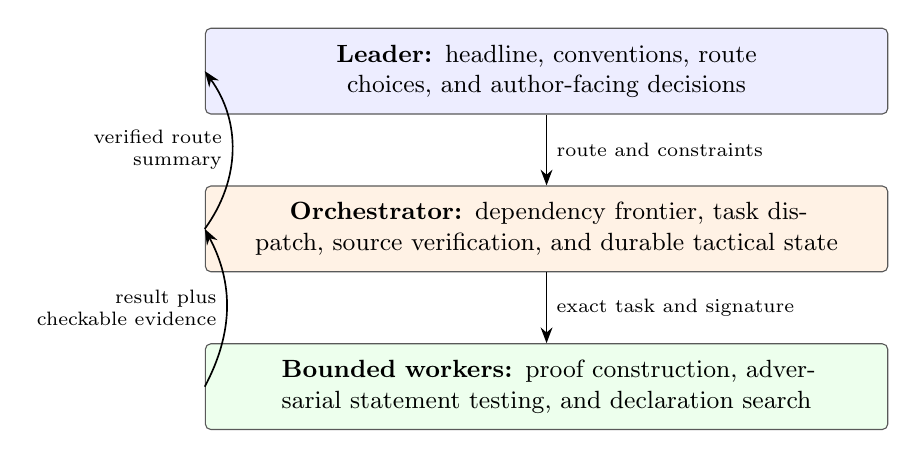
\begin{tikzpicture}[
  node distance=9mm,
  box/.style={draw=black!65,rounded corners=2pt,align=center,
    font=\small,text width=.68\textwidth,inner sep=6pt},
  arrow/.style={-{Stealth[length=2mm]},semithick}
]
\node[box,fill=blue!7] (leader) {\textbf{Leader:} headline, conventions,
  route choices, and author-facing decisions};
\node[box,fill=orange!10,below=of leader] (orch) {\textbf{Orchestrator:}
  dependency frontier, task dispatch, source verification, and durable tactical state};
\node[box,fill=green!7,below=of orch] (workers) {\textbf{Bounded workers:}
  proof construction, adversarial statement testing, and declaration search};
\draw[arrow] (leader) -- node[right,font=\scriptsize] {route and constraints} (orch);
\draw[arrow] (orch) -- node[right,font=\scriptsize] {exact task and signature} (workers);
\draw[arrow] (workers.west) to[bend right=28]
  node[left,font=\scriptsize,align=right] {result plus\\checkable evidence} (orch.west);
\draw[arrow] (orch.west) to[bend right=36]
  node[left,font=\scriptsize,align=right] {verified route\\summary} (leader.west);
\end{tikzpicture}
\caption{Separation of mathematical direction, tactical coordination, and
bounded proof work.  Evidence flows upward only after comparison with source
and Lean output.}
\label{fig:auto-formalization-three-tier}
\end{figure}

\subsection{Consumer-driven top-down descent}

The method begins with the desired headline signature rather than with a large
collection of preparatory lemmas.  The current node is first attacked directly.
If a prerequisite is missing, the parent proof is drafted with a typed hole;
Lean's proof state is then used to expose the exact proposition the parent
consumes.  That proposition becomes a named child declaration in its intended
source file, and the parent is compiled from the child before descent
continues.  During this transient stage the child may have a \texttt{sorry}
body.  The placeholder marks the current frontier: it shows that the parent
\emph{assembles} from the child, but it does not show that the child is true.

This distinction gives two separate certificates.  A compiling glue proof
certifies that the children jointly imply the parent.  Only a proof term for
each child certifies the mathematical leaves.  The frontier therefore moves
downward until every declaration reachable from the headline is either an
existing checked theorem or a newly completed proof.  Temporary placeholders
outside the final transitive dependency closure are a repository-quality
issue, but they are not axioms of the headline theorem.

Child statements are kept \emph{consumer-minimal}: their strength and domain
are read from the proof that uses them, rather than chosen for aesthetic
generality.  This reduces several recurrent failure modes---for example,
demanding a pointwise estimate when only an integrated estimate is available,
quantifying over a larger time interval than the hypotheses control, or
asserting separate regularity when only joint regularity has been established.
Before a new child is introduced, the workflow searches both the project and
\texttt{mathlib}; formalizing an already available theorem under a new name is
neither useful nor harmless in a large dependency graph.

The short-time proof illustrates this descent.  The headline reduces to a
jointly regular Ricci--DeTurck solution, a smooth family of conjugating
diffeomorphisms, pullback naturality, and a theorem closing the PDE at $t=0$.
The Ricci--DeTurck node reduces in turn to the spectral maximal-regularity
engine, nonlinear estimates, metric realization, all-order regularity, and the
geometric representation identity.  These are mathematical dependencies, not
chapters invented after the code was complete: their formal signatures were
fixed by how the parent proof uses them.

\subsection{Adversarial statement review}

Proving a formally stated theorem and checking that it is the intended theorem
are different tasks.  A refuter is therefore assigned the null hypothesis that
a proposed statement is false, vacuous, or mis-scoped.  It searches for
degenerate witnesses, unconstrained families, endpoint errors, missing
nonzero hypotheses, and conclusions stronger than the available estimates.
When possible, a claimed counterexample is expressed as runnable Lean source.
The orchestrator reruns it before any statement is changed.

Refutation is most valuable at the birth of a load-bearing signature.  It
cannot replace proof: failure to find a counterexample is not evidence of
truth.  Nor does it replace author review.  In this project, particularly
sensitive interfaces included one-sided time derivatives, chart-to-intrinsic
regularity transfers, positivity of metric perturbations, and limit packages
whose fields could accidentally restate a desired conclusion.  The final
semantic audit of the short-time theorem is given in
Section~\ref{sec:artifact-verification}; the global deferred interfaces are
listed in Section~\ref{sec:dependency-ledger}.

\subsection{Mechanical acceptance gates}

The current protocol treats agent messages as proposals and uses Lean and the
repository as the acceptance layer.  Depending on the task, the orchestrator
checks the edited source, the exact elaborated declaration, a narrow module
build, the project build, and the transitive axiom report.  A refuter's claimed
counterexample is rerun; a researcher's claimed declaration is opened at its
source and its type checked.  Source diffs are inspected to detect accidental
changes outside the assigned task.

For a completed \texttt{/prove} headline, the documented terminal condition is
that the reachable placeholder frontier and the in-scope source sweep are
empty, a fresh warning-free build succeeds, the checkpoint working tree is
clean, and \texttt{\#print axioms} for the headline contains exactly
\[
  [\texttt{propext},\ \texttt{Classical.choice},\ \texttt{Quot.sound}].
\]
The role of these three standard axioms, and the difference between this
theorem-specific result and a repository-wide placeholder scan, are explained
in Section~\ref{sec:artifact-verification}.  In particular, the terminal check
does not infer mathematical meaning from a green build.

\subsection{Human responsibility and scope of automation}

The authors remain responsible for the target theorem, definitions,
conventions, route choices, imported results, and the claim that each formal
signature expresses the mathematics described in this paper.  They also
review which declarations are suitable public interfaces.  This matters here:
the proof-producing agents successfully closed a specialized short-time
endpoint, but some internal PDE capstones still have signatures too entangled
with implementation data to be presented as general theorems.  Kernel
acceptance cannot make such an interface mathematically well designed.

Automated assistance was used for source search, decomposition, proof attempts,
counterexample search, refactoring suggestions, and manuscript drafting.  The
immutable submission release records the final source and machine-checkable
verification data, and
Subsection~\ref{subsec:automated-assistance-disclosure} identifies the
assistance systems and versions.  No
language-model output is part of the trusted proof object.  Once elaboration is
complete, Lean's kernel checks the resulting term using the same rules whether
the term was written by a human, generated by an agent, or assembled from both.


\section{Formal artifact, kernel verification, and trust boundary}
\label{sec:artifact-verification}

Formalization status is a claim about a particular declaration at a particular
source revision.  A successful build, a theorem-specific axiom report, a
repository-wide placeholder scan, and a human comparison between formal and
informal statements answer different questions.  This section records the
evidence supplied for the short-time endpoint, audits the main
ways circular reasoning could be concealed by an otherwise valid Lean term,
and specifies the immutable release record accompanying the submission.

\subsection{Verified short-time endpoint}
\label{subsec:verified-short-time-endpoint}

The immutable submission artifact builds successfully.  For the exact declaration
\leanref{ricci_flow_short_time_existence}, the command
\begin{center}
  \texttt{\#print axioms ricci\_flow\_short\_time\_existence}
\end{center}
returns exactly
\begin{equation}
  [\texttt{propext},\ \texttt{Classical.choice},\ \texttt{Quot.sound}].
  \label{eq:short-time-axioms}
\end{equation}
The command is present immediately after the declaration in
\rffile{Geometry/Flow/RicciFlow/ShortTimeExistence.lean}.  Equation
\eqref{eq:short-time-axioms} is theorem-specific: it reports the axioms used
transitively by the proof term of this declaration.  In particular, the
closure contains neither \texttt{sorryAx} nor a project-defined axiom.

The three reported constants are standard parts of the classical foundation
used throughout \texttt{mathlib}.  Proposition extensionality
(\texttt{propext}) identifies logically equivalent propositions;
\texttt{Classical.choice} supplies a choice function from a proof of
nonemptiness; and \texttt{Quot.sound} identifies related representatives in a
quotient.  Their appearance means that the proof is classical and uses Lean's
quotient foundation.  It does not signal an unfinished mathematical lemma,
and it should not be paraphrased as ``axiom-free'' or ``constructive.''

A green editor marker or successful build gives a related but weaker piece of
evidence.  It shows that Lean elaborated the source and that the kernel accepted
the resulting terms relative to the imported environment.  It does not by
itself reveal whether the theorem depends on a placeholder or custom axiom;
that is why the transitive \texttt{\#print axioms} output is recorded
separately.  Conversely, the axiom report should always be attached to the
exact elaborated signature, since a clean proof of the wrong statement is not
evidence for the intended theorem.

\subsection{Theorem closure, import closure, and repository state}

The theorem-specific axiom report should not be conflated with two broader
questions about the environment in which the theorem was compiled.  A
declaration can have a clean transitive axiom set even when its imported
environment contains declarations that its proof never uses; still less does
that report classify unrelated files elsewhere in the repository.  Conversely,
a source-tree scan cannot establish either the precise dependency closure or
the mathematical adequacy of an advertised theorem.  The release audit
therefore computes each scope directly rather than inferring dependencies from
directory layout or textual proximity.

Three levels of audit should consequently not be conflated:

\begin{enumerate}[leftmargin=2em]
  \item A \emph{theorem-specific audit} records the exact type and transitive
  axioms of one advertised endpoint.
  \item An \emph{import-closure audit} inspects all declarations made available
  while compiling that endpoint, whether or not its proof term uses them.
  \item A \emph{repository audit} searches every project source for
  placeholders, declared axioms, unsafe escape hatches, and generated or
  vendored code that requires separate provenance.
\end{enumerate}

Equation~\eqref{eq:short-time-axioms} answers the first question for the
short-time theorem.  It is not, by itself, a certification of the other two
scopes.  The audit record in Subsection~\ref{subsec:immutable-release} reports
all three checks and the commands used to obtain them.

\subsection{Kernel verification and semantic circularity}
\label{subsec:kernel-circularity}

Lean rules out ordinary proof-term cycles.  A nonrecursive declaration can
refer only to constants already admitted to the environment; mutually
recursive declarations are accepted only through Lean's checked recursion
mechanisms.  Recursive definitions must pass the required termination or
productivity checks, and a theorem cannot be proved by an arbitrary
nonterminating self-call.  A hidden \texttt{sorry} is represented by
an axiom and appears transitively as \texttt{sorryAx}.  In these syntactic and
type-theoretic senses, kernel checking detects the usual forms of circular
proof construction.

It cannot detect \emph{semantic} circularity caused by a poorly designed
statement.  Lean correctly proves $P\to P$ by returning its hypothesis;
likewise, a structure supplied as an input may already contain a field
equivalent to the conclusion later projected from it.  The kernel also cannot
decide that a formal definition of ``Ricci flow,'' ``strictly parabolic,'' or
``Cheeger--Gromov limit'' is weaker than the mathematical concept intended by
the authors.  These are theorem-design and interpretation questions, and they
require a human audit of signatures and proof data.

We performed that semantic audit adversarially for the short-time chain.  The
headline assumes only the manifold structure, compactness and
boundarylessness, positive dimension, and the initial smooth metric.  It does
not assume a Ricci-flow family, a DeTurck solution, an existence theorem, or a
regularity conclusion.  The all-orders forcing condition consumed by the
specialized nonlinear capstone is proved for the actual symmetrized DeTurck
nonlinearity by \leanref{deTurckRicci_forcingBootstrap_symm}; it is not promoted
to a headline hypothesis.  The forcing-ball retraction and the radial
metric-cone scaling are both proved inactive at the constructed fixed point.
The metric representation theorem then identifies the abstract tensor
solution with the genuine DeTurck right-hand side.  Gauge removal uses an ODE
for diffeomorphisms and Ricci pullback naturality, and the $t=0$ equation is
proved from interior evolution and continuity by
\leanref{ricci_flow_pde_at_zero}.  We found no field or hypothesis in this
chain that merely packages the desired Ricci-flow conclusion back into the
proof.

The audit also corrected a tempting but false description of the proof route.
A generic locally-Lipschitz existence theorem is present in the wider
development, but it is not called by the final short-time chain.  The actual
producer uses the symmetrized, radially controlled Sobolev nonlinearity and the
forcing-space fixed point described in
Subsection~\ref{subsec:short-time-nonlinear}.  Similarly, the outer definition
of \leanref{IsStrictlyParabolicMetricRHS} packages a
\leanref{HasPrincipalSymbol} witness.  That inner specification contains the
pointwise negative-isotropic identity and positivity for nonzero covectors,
but not a separate uniform-neighborhood estimate.  The analytic solution is
obtained by explicit estimates, not by projecting existence from the outer
predicate.

\subsection{Immutable submission release}
\label{subsec:immutable-release}

The formal artifact accompanying this paper is the following immutable project
release:
\begin{center}
\begin{tabular}{@{}rl@{}}
Repository: & \url{https://github.com/qinz1yang/differential-geometry} \\
Release: & \textcolor{red}{\texttt{[INSERT RELEASE URL]}} \\
Release tag: & \textcolor{red}{\texttt{[INSERT RELEASE TAG]}} \\
Commit: & \textcolor{red}{\texttt{[INSERT FULL COMMIT SHA]}} \\
Archive record: & \textcolor{red}{\texttt{[INSERT DOI OR ARCHIVE IDENTIFIER]}} \\
Source index: & \textcolor{red}{\texttt{[INSERT COMMIT-PINNED SOURCE INDEX]}} \\
Audit record: & \textcolor{red}{\texttt{[INSERT AUDIT REPORT LOCATION]}}
\end{tabular}
\end{center}
A branch head and a movable tag are not archival anchors; throughout this
paper, the release and full commit SHA above are the normative source revision.
The artifact was checked from a clean checkout with
\textcolor{red}{\texttt{[INSERT LEAN TOOLCHAIN]}} and
\texttt{mathlib} revision
\textcolor{red}{\texttt{[INSERT MATHLIB COMMIT]}} using
\begin{center}
  \textcolor{red}{\texttt{[INSERT CLEAN-BUILD COMMAND]}}.
\end{center}
The command completed successfully.  Its complete log is preserved at
\textcolor{red}{\texttt{[INSERT BUILD-LOG LOCATION OR CHECKSUM]}}.

The release record contains:

\begin{itemize}[leftmargin=2em]
  \item the release URL, tag, immutable commit SHA, and archive identifier
  listed above;
  \item the pinned Lean toolchain and \texttt{mathlib} revision;
  \item the clean-build command, its successful exit status, and the complete
  build log;
  \item the exact elaborated types and \texttt{\#print axioms} output for every
  advertised endpoint;
  \item the theorem dependency closure and separate import-closure and
  repository-wide scans for \texttt{sorry}, \texttt{axiom}, \texttt{unsafe},
  and comparable trust-relevant mechanisms;
  \item stable source links for every declaration signature displayed in this
  paper, together with licensing and vendoring provenance.
\end{itemize}

Every displayed signature, source path, dependency classification, and status
assertion in this manuscript was reconciled with that release.  Model-space
assumptions were checked declaration by declaration; in particular, the
normed-model-space signature of the headline short-time theorem is not used to
infer a stronger project-wide generality claim.  The exact build and axiom
record in Subsection~\ref{subsec:verified-short-time-endpoint} is therefore tied
to an inspectable, immutable source artifact rather than to a moving
development branch.

\subsection{Automated assistance disclosure}
\label{subsec:automated-assistance-disclosure}

The workflow described in Section~\ref{sec:auto-formalization-workflow} used
language-model agents for declaration search, proof decomposition, Lean proof
attempts, adversarial statement testing, debugging and refactoring proposals.
Language-model assistance was also used in drafting and revising the
manuscript, including the interleaved explanations of formal signatures.  All
such material remains subject to author review against the source and the
mathematics.

The systems and versions used were
\textcolor{red}{\texttt{[INSERT SYSTEM AND VERSION DISCLOSURE]}}.  The project
record distinguishes code generation, search, review, and prose assistance.
This disclosure concerns provenance and research practice; it does not add an
item to the proof's trusted computing base.  The authors retain responsibility
for the statements, proofs, status classifications, citations, and exposition.


\section{Conclusion}

This paper presents the mathematical architecture and current verified stage
of a Lean formalization program for Hamilton's three-manifold theorem.  The
short-time Ricci-flow existence declaration is a closed, theorem-specifically
audited milestone; its proof develops a spectral Sobolev and maximal-regularity
engine, solves the Ricci--DeTurck equation, and removes the gauge through a
jointly smooth diffeomorphism family.  The development also contains
substantial differential-geometric, evolution, weak maximum-principle, and
pinching layers.  All source-level claims are synchronized with the immutable
submission release recorded in Subsection~\ref{subsec:immutable-release}.

The paper does not claim an unconditional Lean proof of Hamilton's theorem.
The metric assembly \leanref{ham3_const_metric} remains
placeholder-dependent on the analytic, compactness, and transfer inputs listed
in Table~\ref{tab:status-at-a-glance} and the dependency ledger.  The augmented
endpoint \leanref{ham3_main} additionally uses the unfinished
spherical-space-form handoff.  The present contribution is a detailed
mathematical explanation of the later blow-up route, an account of the
formalization choices and project-local layers, and an explicit map
of the remaining boundary.

The immutable artifact records the compilation, placeholder, dependency,
axiom, and reproducibility checks described in
Section~\ref{sec:artifact-verification}.  The status qualifications in this
paper follow those recorded results.

\section*{Acknowledgments}

\textcolor{red}{[We will edit this later.]}

This formalization is built on the Lean~4 proof assistant and the
\texttt{mathlib} library \cite{deMouraUllrichLean4,mathlib}, and it would not exist
without the sustained work of the \texttt{mathlib} community.  Beyond that
general debt, the development directly consumes several identifiable bodies of
work, and we wish to acknowledge their authors specifically; published
accounts and expository materials on the relevant differential-geometric
foundations include
\cite{GouezelHigherOrderCalculus,BordgCavalleriDGLean,RothgangDGMathlib,
MassotVanDoornNashSphereEversion}.  The module-level attributions below reflect
the frozen source history of the immutable artifact identified in
Subsection~\ref{subsec:immutable-release}.  The manifold,
charted-space, and smooth-map infrastructure on which every geometric object
here is built is due in large part to S\'ebastien Gou\"ezel, Floris van Doorn,
Heather Macbeth, Yury Kudryashov, and Patrick Massot; the tangent- and
vector-bundle layers to Floris van Doorn, Heather Macbeth, Nicol\`o Cavalleri,
S\'ebastien Gou\"ezel, Patrick Massot, and Michael Rothgang; and the bundled
covariant-derivative interface that our Levi-Civita construction instantiates
to Patrick Massot, Michael Rothgang, and Heather Macbeth.  The
Riemannian-metric modules underlying our smooth-metric type are due to
S\'ebastien Gou\"ezel.  The spectral theorem for compact self-adjoint
operators at the core of our spectral Sobolev engine is due to Heather
Macbeth, with the surrounding inner-product-space and adjoint theory due to
Fr\'ed\'eric Dupuis, Zhouhang Zhou, S\'ebastien Gou\"ezel, and others.  The
Picard--Lindel\"of and integral-curve theory consumed by the gauge-removal
step is due to Winston Yin and Yury Kudryashov.  The Bochner-integration and
$L^p$/$L^2$ layers used throughout the analytic development are due to R\'emy
Degenne, Zhouhang Zhou, Yury Kudryashov, and S\'ebastien Gou\"ezel, and the
multilinear-map and operator-norm infrastructure behind the tensor model
fibers to S\'ebastien Gou\"ezel, Sophie Morel, Yury Kudryashov, Jan-David
Salchow, and Jean Lo.  For the calculus and topology foundations we thank,
among many others, Jeremy Avigad, Johannes H\"olzl, Mario Carneiro, Gabriel
Ebner, and Anatole Dedecker.  These lists are necessarily incomplete, and we
thank the many further \texttt{mathlib} contributors, maintainers, and
reviewers whose work we use on every page.

We are especially grateful to Scott Armstrong and Julia Kempe.  The project
vendors their formalization of interior
De~Giorgi--Nash--Moser theory \cite{ArmstrongKempeDGNM}, with import-path
adaptations, in the project's \texttt{External/} directory; it supplies the
Euclidean Sobolev substrate of the project-local Rellich--Kondrachov step in the
short-time existence engine.  The vendored source is based on upstream revision
\textcolor{red}{\texttt{[INSERT DGNM UPSTREAM REVISION]}}; its local
modifications and license notices are recorded at
\textcolor{red}{\texttt{[INSERT DGNM PROVENANCE FILE OR URL]}}.
Finally, we thank the Lean developers and the Lean Focused Research
Organization for the Lean proof assistant itself.
\clearpage
\appendix
\section{Background formulas and auxiliary derivations}

This appendix records textbook background and auxiliary derivations used by the
main text.  It is explanatory rather than a theorem-to-Lean status ledger: a
displayed formula here should not be read as a claim that the project contains a
separate final Lean theorem with exactly that statement.
Table~\ref{tab:status-at-a-glance} and
Remark~\ref{rem:status-evidence} give the authoritative manuscript-level
status summary.  The main-text proof paragraphs elaborate the mathematical
scope of individual results as audited in the immutable source artifact.

Links below point to the relevant public \texttt{mathlib} documentation from their first occurrences.

\subsection{Basic Riemannian geometry}\label{subsec:BasicRiemGeom}

The fundamental hierarchy of structures in Riemannian geometry is
\[
g \;\longrightarrow\; \nabla \;\longrightarrow\; \Rm ,
\]
where the \href{https://leanprover-community.github.io/mathlib4_docs/Mathlib/Geometry/Manifold/VectorBundle/Riemannian.html}{Riemannian metric} determines the Levi-Civita \href{https://leanprover-community.github.io/mathlib4_docs/Mathlib/Geometry/Manifold/VectorBundle/CovariantDerivative/Basic.html}{connection} and the connection
determines the curvature tensor.

\subsubsection{Levi-Civita, Riemann, Ricci, and scalar curvature}


The Levi-Civita connection
$\nabla: \mathfrak{X}(M) \times \mathfrak{X}(M) \to \mathfrak{X}(M)$
is the unique linear connection on the tangent bundle $TM$ that is both
torsion-free and metric-compatible.  The project-local construction and its
relationship to the surrounding library API are described in the main text.
The \textbf{Koszul formula} for
$\nabla$ is
\begin{align}
 2g\left(  \nabla_{U}V,W\right)   &  =U\left(  g\left(  V,W\right)  \right)
+V\left(  g\left(  U,W\right)  \right)  -W\left(  g\left(  U,V\right)  \right)
\nonumber \\
&   -g\left( U,  \left[  V,W\right] \right) -g\left( V, \left[  U,W\right]
\right)    + g\left( W, \left[  U,V\right]  \right)   .   \label{eq:koszul-formula}
\end{align}
The standard derivation expands the first line of
\eqref{eq:koszul-formula}, uses metric compatibility, and cancels the
remaining terms with the torsion-free condition.

\begin{definition}[Christoffel symbols]
\label{def:Christoffel_symbols}
    Let $(M,g)$ be a Riemannian manifold and let $(U,\mathbf{x})$ be a
    local coordinate chart, with $\mathbf{x}=(x^1,\dots,x^n)$.  Let
    $\{\partial_i\}_{i=1}^n$ denote the induced coordinate frame on
    $TM|_U$, where $\partial_i:=\frac{\partial}{\partial x^i}$.

    If $\nabla$ is the Levi-Civita connection of $g$, the
    \textbf{Christoffel symbols} are the functions
    $\Gamma_{ij}^k:U\to\mathbb R$ defined by expanding the covariant
    derivative in this coordinate frame:
    \begin{equation}
        \nabla_{\partial_i} \partial_j = \Gamma_{ij}^k \partial_k,
    \end{equation}
    where the Einstein summation convention is implied over the index $k$.
\end{definition}

The Christoffel symbols can be expressed in terms of the first partial
derivatives of the metric components:
\begin{equation}\label{eq:ChristoffelSymbols0th}
        \Gamma_{ij}^k = \frac{1}{2} g^{kl} \left( \partial_i g_{jl} + \partial_j g_{il} - \partial_l g_{ij} \right) ;
    \end{equation}
this follows from \eqref{eq:koszul-formula} and the fact that $[\partial_i,\partial_j]=0$.

The Riemann curvature tensor is defined by
\begin{equation}\label{eq:riemann-curvature-definition}
   R(X,Y)Z := \nabla_X (\nabla_Y Z) - \nabla_Y (\nabla_X Z) - \nabla_{[X,Y]} Z .
\end{equation}

The components of the Riemann curvature tensor are defined by
\begin{equation}
    R_{ijk}^l \partial_l = R(\partial_i,\partial_j)\partial_k .
\end{equation}
Using
\begin{equation*}
    \nabla_{\partial_i}(\nabla_{\partial_j}\partial_k) = \nabla_{\partial_i}(\Gamma_{jk}^\ell \partial_\ell)
    = \partial_i \Gamma_{jk}^{\ell}
+ \Gamma_{jk}^p \nabla_{\partial_i}\partial_p ,
\end{equation*}
we compute that
    \begin{equation}\label{eq:riemann-curvature-components}
        R_{ijk}^{\ell} = \partial_i \Gamma_{jk}^{\ell} - \partial_j \Gamma_{ik}^{\ell} + \Gamma_{jk}^{p}\Gamma_{ip}^{\ell} - \Gamma_{ik}^{p}\Gamma_{jp}^{\ell}.
    \end{equation}

As a $(0,4)$-tensor, $\Rm$ is defined by
\begin{equation}
    \Rm(X,Y,Z,W) := \langle R(X,Y)Z,W \rangle .
\end{equation}
Its components are defined by
\begin{equation}
    R_{ijkl} :=\Rm(\partial_i,\partial_j,\partial_k,\partial_l) .
\end{equation}
Raising and lowering the final index gives
\begin{equation}
    R_{ijkl}=R_{ijk}^m g_{ml} \quad \text{and} \quad R_{ijk}^l = R_{ijkm} g^{ml} .
\end{equation}

The dimension-three Riemann-from-Ricci identity, together with its Lean-facing
status and curvature convention, is stated once in
Lemma~\ref{lem:3d-curvature-identities} and is not repeated here.

\subsection{Tensor calculus}\label{subsec:TensorCalculus}

\subsubsection{Tensors}

Many geometric quantities appearing in Riemannian geometry---such as the metric,
curvature, and their covariant derivatives---are naturally expressed as tensors.

\begin{definition}[$(r,s)$-tensor]
\label{def:rs_tensor}
    Let $M$ be a smooth manifold and let $p\in M$.  Let $T_pM$ be
    the tangent space and let $T_p^*M$ be the cotangent space at $p$.

    An \textbf{$(r,s)$-tensor} at $p$ is a multilinear map
    \begin{equation}
        T: \underbrace{T_p^* M \times \dots \times T_p^* M}_{r \text{ times}} \times \underbrace{T_p M \times \dots \times T_p M}_{s \text{ times}} \to \mathbb{R}.
    \end{equation}
    Thus $T$ takes $r$ covectors and $s$ vectors as input, returns a real
    number, and is linear in each argument.

    A \textbf{smooth $(r,s)$-tensor field} is a smooth assignment of such a
    multilinear map to every point $p\in M$.  Equivalently, it can be viewed
    as a $C^\infty(M)$-multilinear map from $r$ smooth $1$-forms and $s$
    smooth vector fields to smooth functions:
    \begin{equation}
        T: \Omega^1(M)^r \times \mathfrak{X}(M)^s \to C^\infty(M),
    \end{equation}
where $\Omega^1(M)$ denotes the space of smooth $1$-forms and
$\mathfrak{X}(M)$ the space of smooth vector fields on $M$.
\end{definition}

\subsubsection{Covariant differentiation of tensors}


Since the Levi-Civita connection is defined on vector fields, we first extend
the notion of covariant differentiation to covariant objects, beginning with
1-forms.

\begin{definition}[Covariant derivative of a $1$-form]
\label{def:cov_dev_1form}
    Let $\nabla$ denote the Levi-Civita connection on $(M,g)$.  Let
    $\omega\in\Omega^1(M)$ be a smooth $1$-form and let
    $X,Y\in\mathfrak{X}(M)$.  The \textbf{covariant derivative} of
    $\omega$ in the direction $X$, denoted $\nabla_X\omega$, is the
    $1$-form defined by
    \begin{equation}
        (\nabla_X \omega)(Y) = X(\omega(Y)) - \omega(\nabla_X Y).
    \end{equation}
Equivalently, this is the product rule for the scalar function
$\omega(Y)$, with the correction term accounting for the variation of the
input vector field $Y$.
\end{definition}

The same rule extends to any smooth $(r,s)$-tensor field $T$.  Since
$\nabla_X$ already acts on functions, vector fields, and $1$-forms, the
general formula is dictated by the Leibniz rule:

\begin{definition}[Covariant derivative of an $(r,s)$-tensor]
\label{def:cov_dev_general}
    We extend the covariant derivative to a smooth $(r,s)$-tensor field $T$
    by requiring that $\nabla_X$ act as a derivation with respect to tensor
    contraction.  Explicitly, for any $X\in\mathfrak{X}(M)$, $r$
    $1$-forms $\omega^1,\dots,\omega^r$, and $s$ vector fields
    $Y_1,\dots,Y_s$, the tensor $\nabla_XT$ is defined by
    \begin{align}
        (\nabla_X T)(\omega^1, \dots, \omega^r, Y_1, \dots, Y_s) &= X \big( T(\omega^1, \dots, \omega^r, Y_1, \dots, Y_s) \big) \nonumber \\
        &\quad - \sum_{k=1}^r T(\omega^1, \dots, \nabla_X \omega^k, \dots, \omega^r, Y_1, \dots, Y_s) \nonumber \\
        &\quad - \sum_{l=1}^s T(\omega^1, \dots, \omega^r, Y_1, \dots, \nabla_X Y_l, \dots, Y_s).
    \end{align}
This is the corresponding product rule for tensor evaluation: each input
slot contributes a correction term.

    The \textbf{total covariant derivative} $\nabla T$ is the $(r,s+1)$-tensor
    field obtained by viewing the differentiation direction as an additional
    vector input.  Covector inputs precede vector inputs, and within the vector
    inputs the differentiation slot comes first:
    \begin{equation}
        (\nabla T)(\omega^1,\dots,\omega^r;X,Y_1,\dots,Y_s)
        :=(\nabla_XT)(\omega^1,\dots,\omega^r;Y_1,\dots,Y_s).
    \end{equation}
\end{definition}

\begin{remark}
    Observe that if $T$ is a $(0,1)$-tensor (a 1-form), the general definition agrees with Definition \ref{def:cov_dev_1form}. In this case ($r=0, s=1$), the first summation is empty, and the formula reduces to
    \begin{equation}
        (\nabla_X T)(Y_1) = X(T(Y_1)) - T(\nabla_X Y_1),
    \end{equation}
    which is exactly the definition of the covariant derivative of a 1-form.
\end{remark}

Since estimates for higher derivatives of the metric in local coordinates
are obtained by controlling covariant derivatives of curvature, we introduce
iterated covariant derivatives of tensor fields.

\begin{definition}[Higher covariant derivatives]
\label{def:high_order_cov_dev}
    We define the $k$-th covariant derivative of a smooth $(r,s)$-tensor field $T$ recursively.

    For $k=0$, we set $\nabla^{(0)} T = T$. For $k \geq 1$, the $k$-th covariant derivative $\nabla^{(k)} T$ is the $(r, s+k)$-tensor field defined as the total covariant derivative of the $(k-1)$-th derivative:
    \begin{equation}
        \nabla^{(k)} T := \nabla (\nabla^{(k-1)} T).
    \end{equation}
    In terms of arguments, if $T$ is a $(0,s)$-tensor, this recursion implies that
    \begin{equation}
        (\nabla^{(k)} T)(X_1, \dots, X_k, Y_1, \dots, Y_s) = (\nabla_{X_1} (\nabla^{(k-1)} T))(X_2, \dots, X_k, Y_1, \dots, Y_s)
    \end{equation}
    for vector fields $X_1, \dots, X_k, Y_1, \dots, Y_s$.
    Note that under this convention, the \emph{first} argument $X_1$ corresponds to the \emph{outermost} (most recent) differentiation operation.
\end{definition}

\begin{remark}
We compute that
\begin{align*}
    (\nabla^{(2)}Z)(X,Y) & = (\nabla_X (\nabla Z)) (Y) \\
    & = \nabla_X( (\nabla Z)(Y)) - (\nabla Z) (\nabla_X Y) \\
    & = \nabla_X(\nabla_Y Z) - \nabla_{\nabla_X Y} Z
\end{align*}
for vector fields $X,Y,Z$.
Therefore we may rewrite the definition
\eqref{eq:riemann-curvature-definition} of the Riemann curvature tensor as
\begin{equation}
    R(X,Y)Z = (\nabla^{(2)}Z)(X,Y) - (\nabla^{(2)}Z)(Y,X) .
\end{equation}
\end{remark}

\subsubsection{Index notation for tensors}


A choice of local coordinates determines a coordinate basis for the
tangent bundle, allowing tensor fields to be expressed through their
components in index notation.

\begin{definition}[Tensor components and covariant derivatives]
\label{def:tensor_components}
    Let $\alpha$ be a smooth $(0,s)$-tensor field. The \textbf{components} of $\alpha$ in the local frame are the smooth functions defined by:
    \begin{equation}
        \alpha_{i_1 \cdots i_s} := \alpha (\partial_{i_1}, \ldots, \partial_{i_s}).
    \end{equation}
    The $k$-th covariant derivative $\nabla^{(k)} \alpha$ is a $(0, k+s)$-tensor field. We denote its components by the symbol $\nabla_{j_1}\cdots \nabla_{j_k} \alpha_{i_1 \cdots i_s}$, defined as the evaluation of the tensor on the coordinate basis:
    \begin{equation}
        \nabla_{j_1}\cdots \nabla_{j_k} \alpha_{i_1 \cdots i_s} := (\nabla^{(k)}\alpha) (\partial_{j_1}, \ldots, \partial_{j_k}, \partial_{i_1}, \ldots, \partial_{i_s}).
    \end{equation}
\end{definition}

\subsubsection{Ricci identities}

The non-commutativity of the covariant derivative is measured precisely by the Riemann curvature tensor. While this is often defined for vector fields, it extends naturally to all tensor fields. We first establish the action of curvature on 1-forms, then extend it to arbitrary tensors via the derivation principle.

\begin{lemma}[Action of curvature on $1$-forms]
\label{lem:curvature_on_1forms}
    Let $\omega \in \Omega^1(M)$ be a smooth $1$-form and let $X, Y, Z \in \mathfrak{X}(M)$. Then
    \begin{equation}\label{eq:ricci-identity-one-form}
        (\nabla_X \nabla_Y \omega)(Z) - (\nabla_Y \nabla_X \omega)(Z) - (\nabla_{[X,Y]} \omega)(Z) = - \omega(R(X,Y)Z).
    \end{equation}
\end{lemma}

\begin{proof}
By the definition of the dual connection, expanding the two second derivatives
and cancelling the first-derivative terms gives
\[
([\nabla_X,\nabla_Y]\omega)(Z)
=[X,Y](\omega(Z))
-\omega(\nabla_X\nabla_YZ-\nabla_Y\nabla_XZ).
\]
On the other hand,
\[
(\nabla_{[X,Y]}\omega)(Z)
=[X,Y](\omega(Z))-\omega(\nabla_{[X,Y]}Z).
\]
Subtracting and using the definition of $R(X,Y)Z$ proves the formula.
\end{proof}

\begin{remark}
We may rephrase equation \eqref{eq:ricci-identity-one-form} as
\begin{equation}
    (\nabla^{(2)} \omega)(X, Y, Z)
- (\nabla^{(2)} \omega)(Y, X, Z) = - \omega(R(X,Y)Z).
\end{equation}
Equation \eqref{eq:ricci-identity-one-form} says, in local coordinates, that
\begin{equation}\label{eq:ricci-identity-one-form-coordinates}
    \nabla_i \nabla_j \omega_k - \nabla_j \nabla_i \omega_k = - R_{ijk}^m \omega_m = - R_{ijk\ell}g^{\ell m} \omega_m .
\end{equation}
\end{remark}

Generalizing \eqref{eq:ricci-identity-one-form-coordinates} to covariant
tensors, we have:

\begin{theorem}[Ricci identity for $(0,s)$-tensors]
\label{thm:ricci_identity}
    Let $\alpha$ be a smooth $(0,s)$-tensor field. In local coordinates, the commutator of second covariant derivatives is given by:
    \begin{equation}
        \nabla_{i}\nabla_{j}\alpha_{k_{1}\cdots k_{s}} - \nabla_{j}\nabla_{i}\alpha_{k_{1}\cdots k_{s}}
        = - \sum_{q=1}^{s} \sum_{m=1}^n R_{ijk_{q}}^{m} \alpha_{k_{1}\cdots k_{q-1} m k_{q+1}\cdots k_{s}}.
    \end{equation}
\end{theorem}

\begin{proof}
Set
\[
\mathcal R(X,Y):=[\nabla_X,\nabla_Y]-\nabla_{[X,Y]}.
\]
Because the connection obeys the Leibniz rule, $\mathcal R(X,Y)$ acts as a
derivation on the tensor algebra.  Lemma~\ref{lem:curvature_on_1forms} therefore
gives the invariant formula
\[
(\mathcal R(X,Y)\alpha)(Z_1,\dots,Z_s)
=-\sum_{q=1}^s
\alpha(Z_1,\dots,R(X,Y)Z_q,\dots,Z_s).
\]
Taking $X=\partial_i$, $Y=\partial_j$, and $Z_q=\partial_{k_q}$, using
$[\partial_i,\partial_j]=0$ and
$R(\partial_i,\partial_j)\partial_{k_q}
=R_{ijk_q}{}^m\partial_m$, yields the stated coordinate identity.
\end{proof}

\begin{remark}[Ricci identity for $(r,s)$-tensors]
    More generally, if $\beta $ is any $\left(  r,s\right)  $-tensor field, one has the
commutator
\begin{align}
\left[  \nabla_{i},\nabla_{j}\right]  \beta_{k_{1}\cdots k_{s}}^{l_{1}%
\cdots l_{r}}  &  := \nabla_{i}\nabla_{j}\beta_{k_{1}\cdots k_{s}}^{l
_{1}\cdots l_{r}}-\nabla_{j}\nabla_{i}\beta_{k_{1}\cdots k_{s}}^{l_{1}\cdots l_{r}} \nonumber \\
&  =\sum_{p=1}^{r} \sum_{m=1}^n R_{ijm}^{l_{p}}\beta_{k_{1}\cdots k_{s}}^{l_{1}\cdots
l_{p-1}ml_{p+1}\cdots l_{r}}-\sum_{q=1}^{s} \sum_{m=1}^n R_{ijk_{q}}^{m}%
\beta_{k_{1}\cdots k_{q-1}mk_{q+1}\cdots k_{s}}^{l_{1}\cdots l_{r}}. \label{eq:ricci-identity-mixed-tensor}
\end{align}
\end{remark}


For example, for a $(1,1)$-tensor $\beta$, we have
\begin{equation}\label{eq:ricci-identity-one-one-tensor}
    \nabla_i\nabla_j \beta_k^l - \nabla_j \nabla_i \beta_k^l =
    R_{ijm}^l\beta_k^m - R_{ijk}^m \beta_m^l.
\end{equation}

\subsubsection{Inner products and norms of tensors}

\begin{definition}[Tensor inner product]
\label{def:tensor_inner_product}
    Let $(M, g)$ be a Riemannian manifold and let $\alpha, \beta$ be $(0,s)$-tensor fields.
    Their \textbf{inner product} is the scalar function $\langle \alpha, \beta \rangle \in C^\infty(M)$ defined at each point $p$ by contracting with respect to a local orthonormal basis $\{e_k\}_{k=1}^n$:
    \begin{equation}
        \langle \alpha , \beta \rangle := \sum_{k_1, \dots, k_s=1}^{n} \alpha (e_{k_1}, \dots, e_{k_s}) \beta (e_{k_1}, \dots, e_{k_s}).
    \end{equation}
    In general local coordinates, this corresponds to the full contraction:
    \begin{equation}
        \langle \alpha , \beta \rangle = g^{i_1 j_1} \dots g^{i_s j_s} \alpha_{i_1 \dots i_s} \beta_{j_1 \dots j_s}.
    \end{equation}
    The norm of a tensor is defined by
\begin{equation}
    |\alpha|^2 := \langle \alpha, \alpha \rangle ,
\end{equation}
so $|\alpha| = \sqrt{\langle \alpha, \alpha \rangle}$.
\end{definition}

For example, if $T$ is a $(0,s)$-tensor and $k\geq 0$, then
\begin{equation}
    |\nabla^{(k)}T|^2 = g^{i_1 j_1} \cdots g^{i_{s+k} j_{s+k}} \nabla_{i_1}\cdots \nabla_{i_k}T_{i_{k+1} \cdots i_{k+s}} \nabla_{j_1} \cdots \nabla_{j_k}T_{j_{k+1} \cdots j_{k+s}} .
\end{equation}

\subsection{The Laplace operator}

For the purposes of this appendix, the rough Laplacian is recorded as the
metric trace of the second covariant derivative.  The main text explains how
the project realizes such identities through invariant, coordinate, or local
frame interfaces when they are used in Lean.

\subsubsection{The rough Laplacian and the divergence}


The Laplacian is the fundamental second-order differential operator in
geometric analysis, obtained by taking the metric trace of the second
covariant derivative.

\begin{definition}[Rough Laplacian]
\label{def:rough_laplacian}
    Let $(M, g)$ be a Riemannian manifold and let $\alpha$ be a $(0,s)$-tensor field.
    The \textbf{rough Laplacian} $\Delta \alpha$ is defined by the metric trace of the second covariant derivative over its first two arguments:
    \begin{equation}
        \Delta \alpha := \operatorname{tr}_{1,2} \big( \nabla^{(2)} \alpha \big).
    \end{equation}
    Explicitly, if $\{e_k\}_{k=1}^n$ is a local orthonormal frame, this trace is given by
    \begin{equation}
        \operatorname{tr}_{1,2} \big( \nabla^{(2)} \alpha \big) (\cdot, \dots, \cdot) := \sum_{k=1}^n (\nabla^{(2)} \alpha)(e_k, e_k, \cdot, \dots, \cdot).
    \end{equation}
    In local coordinates, this corresponds to the contraction:
    \begin{equation}
        (\Delta \alpha)_{i_1 \dots i_s} = g^{jk} \nabla_j \nabla_k \alpha_{i_1 \dots i_s}.
    \end{equation}
\end{definition}

The divergence is a fundamental first-order operator in geometric
analysis, obtained by taking the metric trace of the covariant derivative.


\begin{definition}[Divergence]
\label{def:divergence}
    Let $(M, g)$ be a Riemannian manifold and let $\alpha$ be a $(0,s)$-tensor field with $s \ge 1$.
    The \textbf{divergence} of $\alpha$ is the $(0,s-1)$-tensor field defined by the metric trace of the covariant derivative $\nabla \alpha$ over its first two arguments:
    \begin{equation}
        \Div(\alpha) := \operatorname{tr}_{1,2} (\nabla \alpha).
    \end{equation}
    In local coordinates, this corresponds to contracting the derivative index with the first index of $\alpha$:
    \begin{equation}
        \big(\Div(\alpha) \big)_{i_2 \dots i_s} = g^{jk} \nabla_j \alpha_{k i_2 \dots i_s}.
    \end{equation}
With respect to an orthonormal frame $\{e_i\}_{i=1}^n$,
\begin{equation}
  \Div(\alpha) = \sum_{i=1}^n (\nabla_{e_i} \alpha ) (e_i,\cdot,\ldots,\cdot) .
\end{equation}
\end{definition}

\begin{remark}[Factorization of the Laplacian]
\label{rem:laplacian_div_grad}
    It follows directly from the definitions that the Laplacian factors as the divergence of the covariant derivative:
    \begin{equation}
        \Delta \alpha = \Div(\nabla \alpha).
    \end{equation}
    Note that this composition is well-typed: if $\alpha$ is a $(0,s)$-tensor, then $\nabla \alpha$ is a $(0,s+1)$-tensor (satisfying the rank requirement for divergence), and the resulting divergence maps it back to a $(0,s)$-tensor.
\end{remark}

\bibliographystyle{amsalpha}
\bibliography{references}

\end{document}
